% Beamer presentation for Reddit-Voat Analysis Results
\documentclass[10pt]{beamer}

% Theme and color settings
\usetheme{default}
\usecolortheme{default}

% Packages
\usepackage{graphicx}
\usepackage{hyperref}

% Title information
\title{Reddit-Voat Analysis Results}
\author{}
\date{October 27, 2025}

\begin{document}

% Title slide
\frame{\titlepage}

% ===================================================================
% ===================================================================
% SECTION: Core-Periphery Analysis: Reddit
% ===================================================================
\section{Core-Periphery Analysis: Reddit}

% -------------------------------------------------------------------
% Funny - Reddit
% -------------------------------------------------------------------
\begin{frame}{Funny - Reddit}
\centering
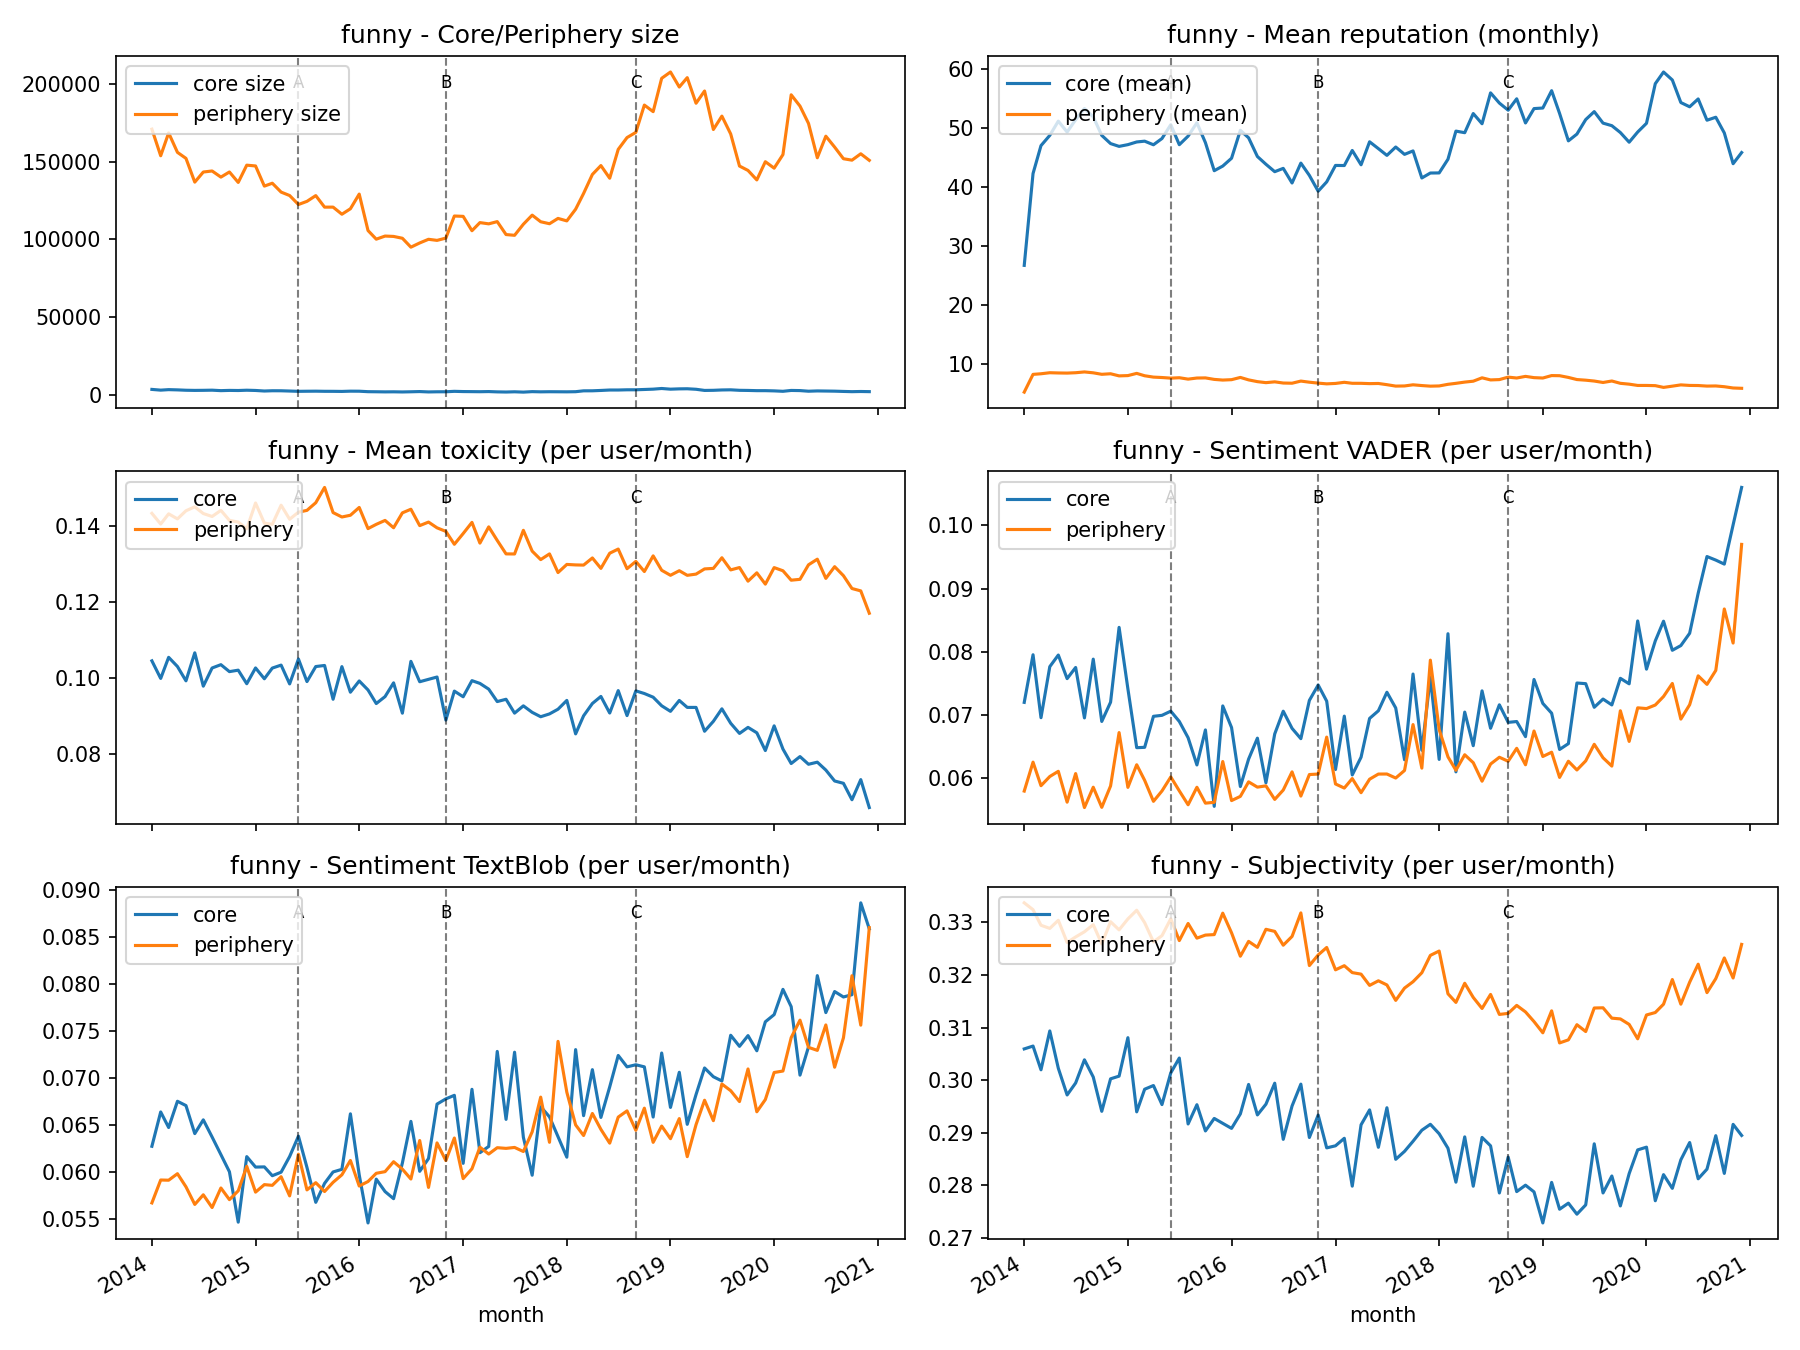
\includegraphics[width=\textwidth]{results/core-periphery/reddit/figures/reddit_funny_cp_panels_2col.png}
\end{frame}

\begin{frame}{Key Insights: Funny - Reddit}
\begin{itemize}
    \item \textbf{Stable core, dynamic periphery}: Core size remains flat ($\sim$5K users) while periphery surges from 100K to 200K at Event C, indicating Reddit retained established contributors but attracted massive new casual engagement
    \item \textbf{Core-periphery toxicity inversion}: Core users maintain lower toxicity (0.07-0.10) than periphery (0.12-0.15), with core declining post-2018—suggesting moderation or norm enforcement from established users
    \item \textbf{Sentiment convergence}: Both core and periphery sentiment trend upward and converge (0.07-0.09) by 2021, possibly reflecting community-wide cultural shift toward more positive engagement
\end{itemize}
\end{frame}

% -------------------------------------------------------------------
% Gaming - Reddit
% -------------------------------------------------------------------
\begin{frame}{Gaming - Reddit}
\centering
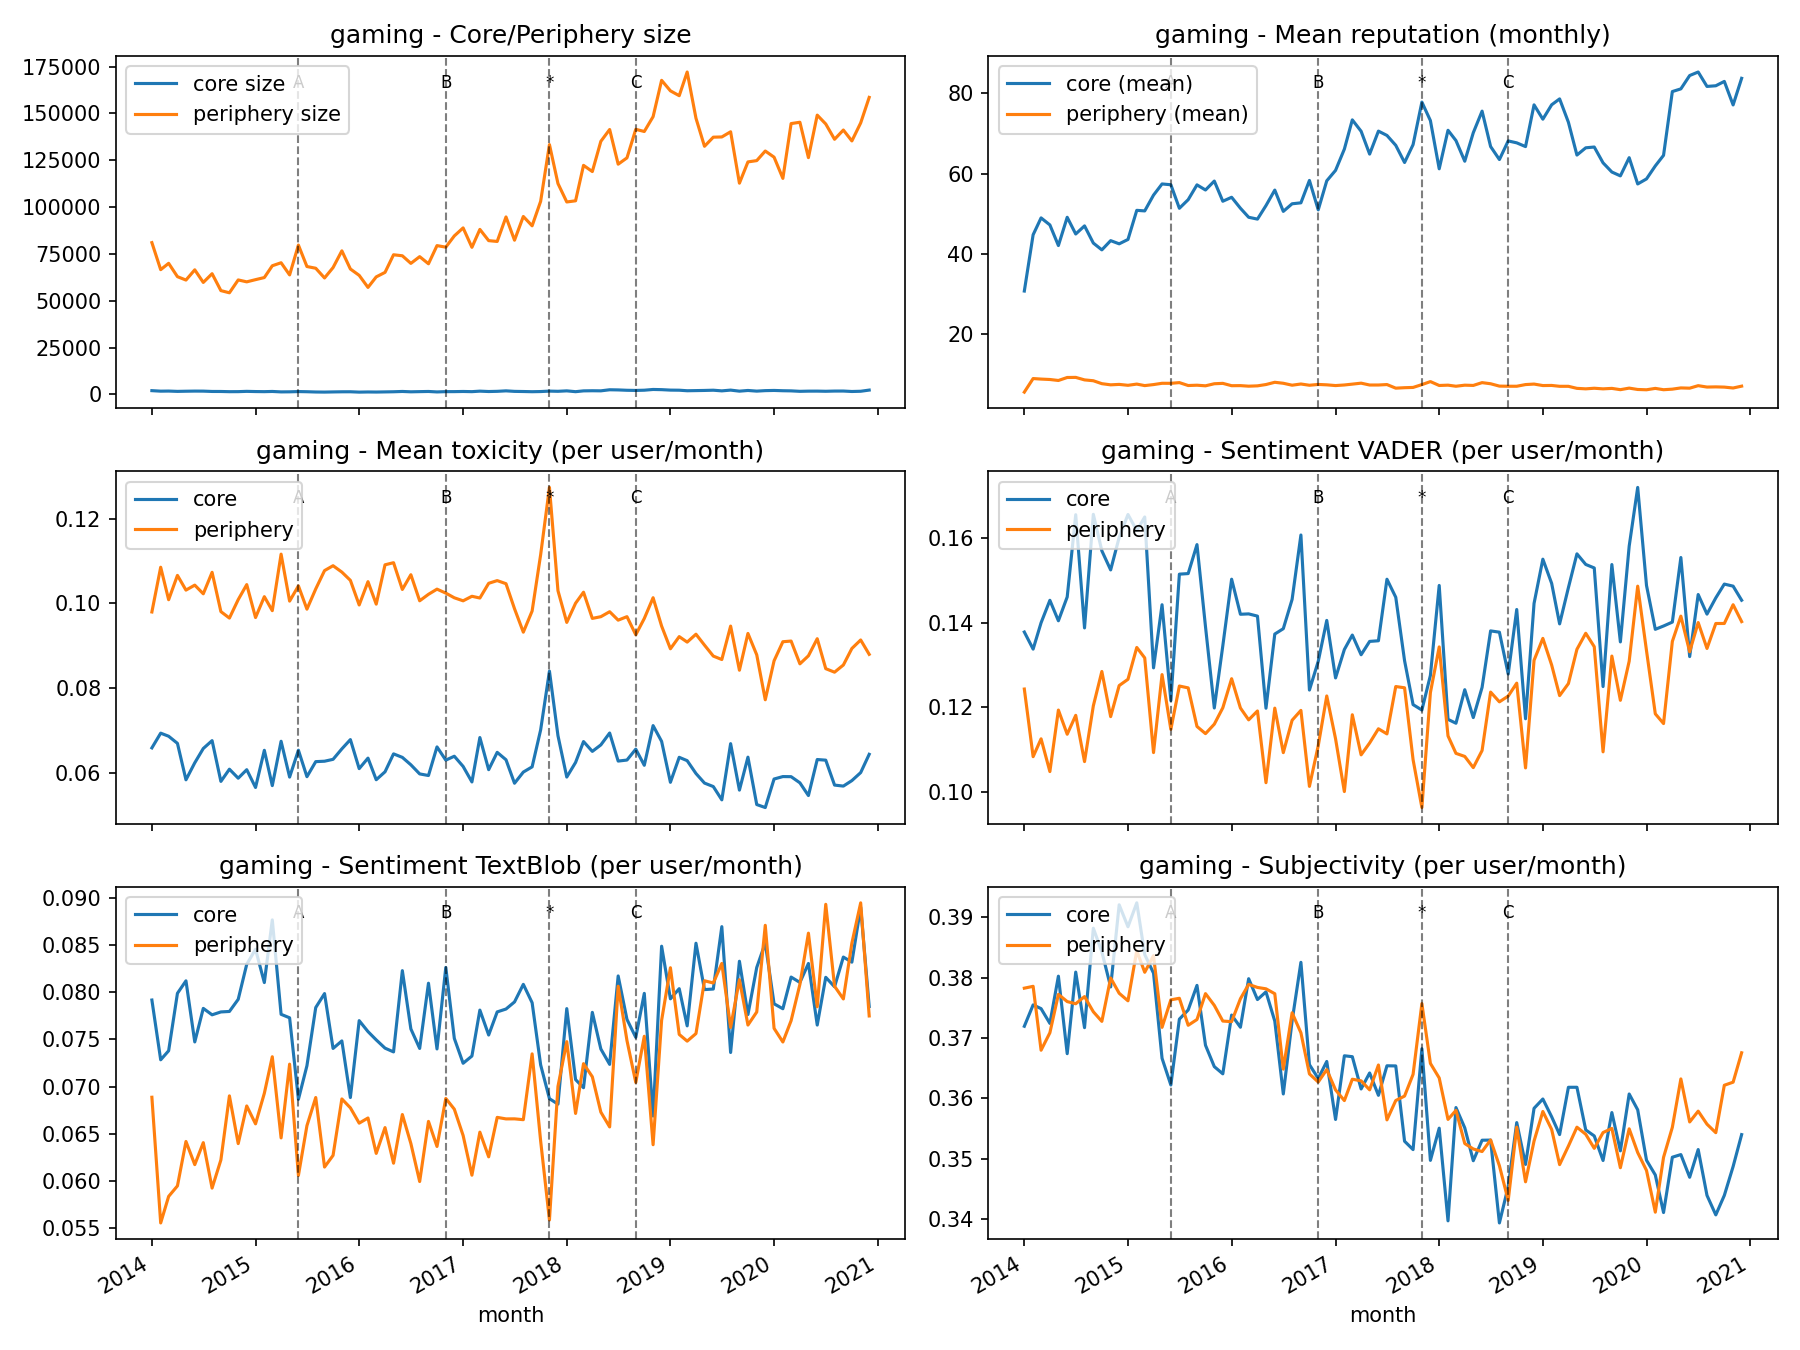
\includegraphics[width=\textwidth]{results/core-periphery/reddit/figures/reddit_gaming_cp_panels_2col.png}
\end{frame}

\begin{frame}{Key Insights: Gaming - Reddit}
\begin{itemize}
    \item \textbf{Periphery explosion at Event C}: Periphery doubles from 75K to 175K at 2018 QAnon ban while core stays flat ($\sim$3K), suggesting Reddit gaming attracted mainstream users fleeing conspiracy-dominated spaces
    \item \textbf{Persistent core advantage}: Core maintains 40-80 reputation (6-8x periphery's $\sim$10) and consistently lower toxicity (0.06 vs 0.10), demonstrating strong hierarchical structure with veteran gatekeepers
    \item \textbf{Sentiment parity with volatility}: Core and periphery show similar sentiment means (0.12-0.14) but core exhibits higher variance spikes, possibly reflecting passionate debates among established users
\end{itemize}
\end{frame}

% -------------------------------------------------------------------
% Gifs - Reddit
% -------------------------------------------------------------------
\begin{frame}{Gifs - Reddit}
\centering
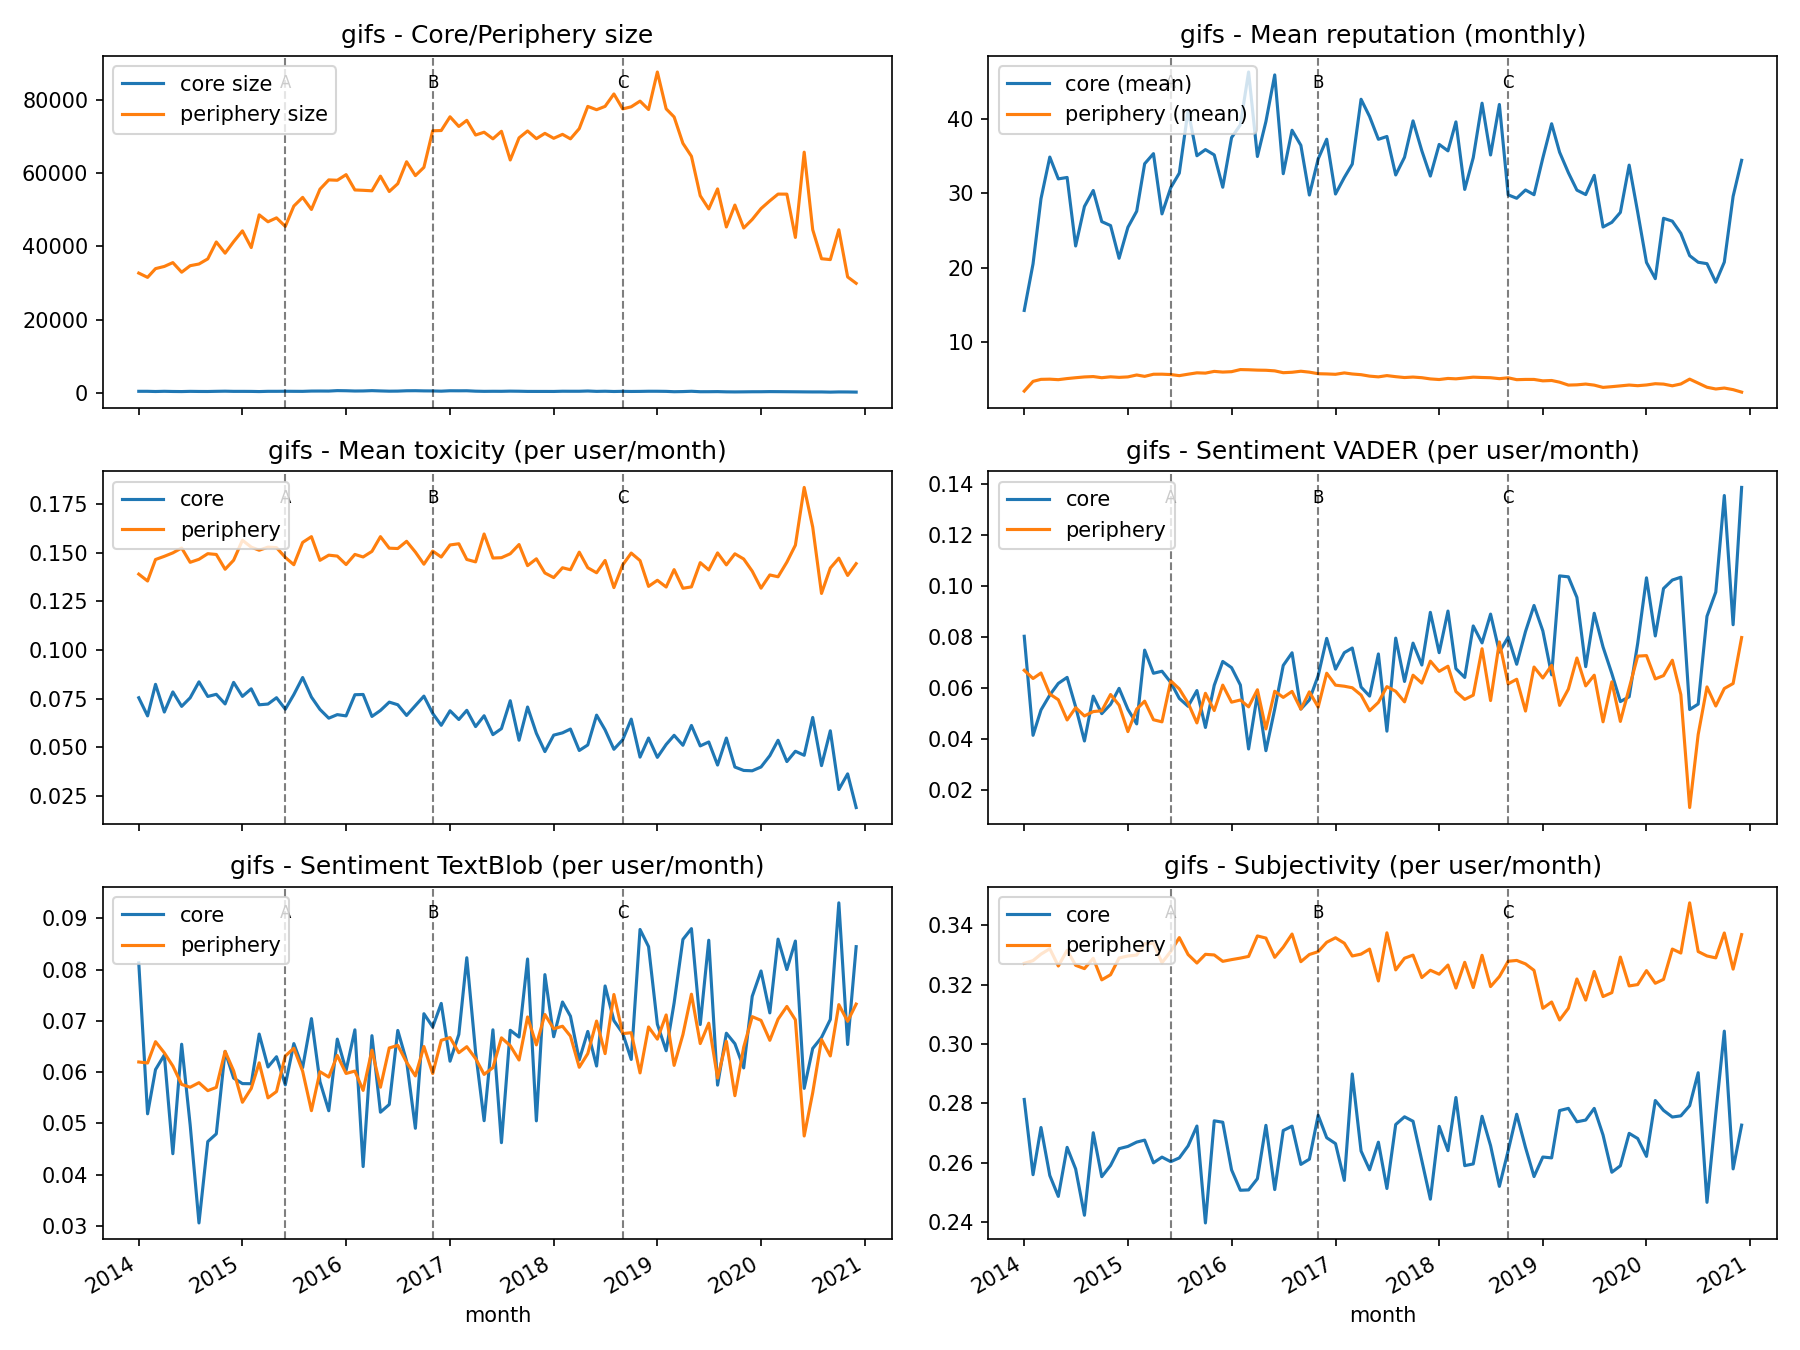
\includegraphics[width=\textwidth]{results/core-periphery/reddit/figures/reddit_gifs_cp_panels_2col.png}
\end{frame}

\begin{frame}{Key Insights: Gifs - Reddit}
\begin{itemize}
    \item \textbf{Post-Event C collapse}: Periphery crashes from 85K peak to 30K by 2021 while core flatlines near zero, suggesting r/gifs lost relevance as video formats displaced static gifs platform-wide
    \item \textbf{Declining core toxicity advantage}: Core toxicity drops from 0.08 to 0.02 by 2021 (falling below periphery's stable 0.14), possibly indicating only the most civil veteran users remained engaged
    \item \textbf{Sentiment divergence at end}: Core sentiment surges to 0.14 in 2021 while periphery drops near zero, reflecting different user cohorts with core becoming small, positive-affect remnant
\end{itemize}
\end{frame}

% -------------------------------------------------------------------
% Pics - Reddit
% -------------------------------------------------------------------
\begin{frame}{Pics - Reddit}
\centering
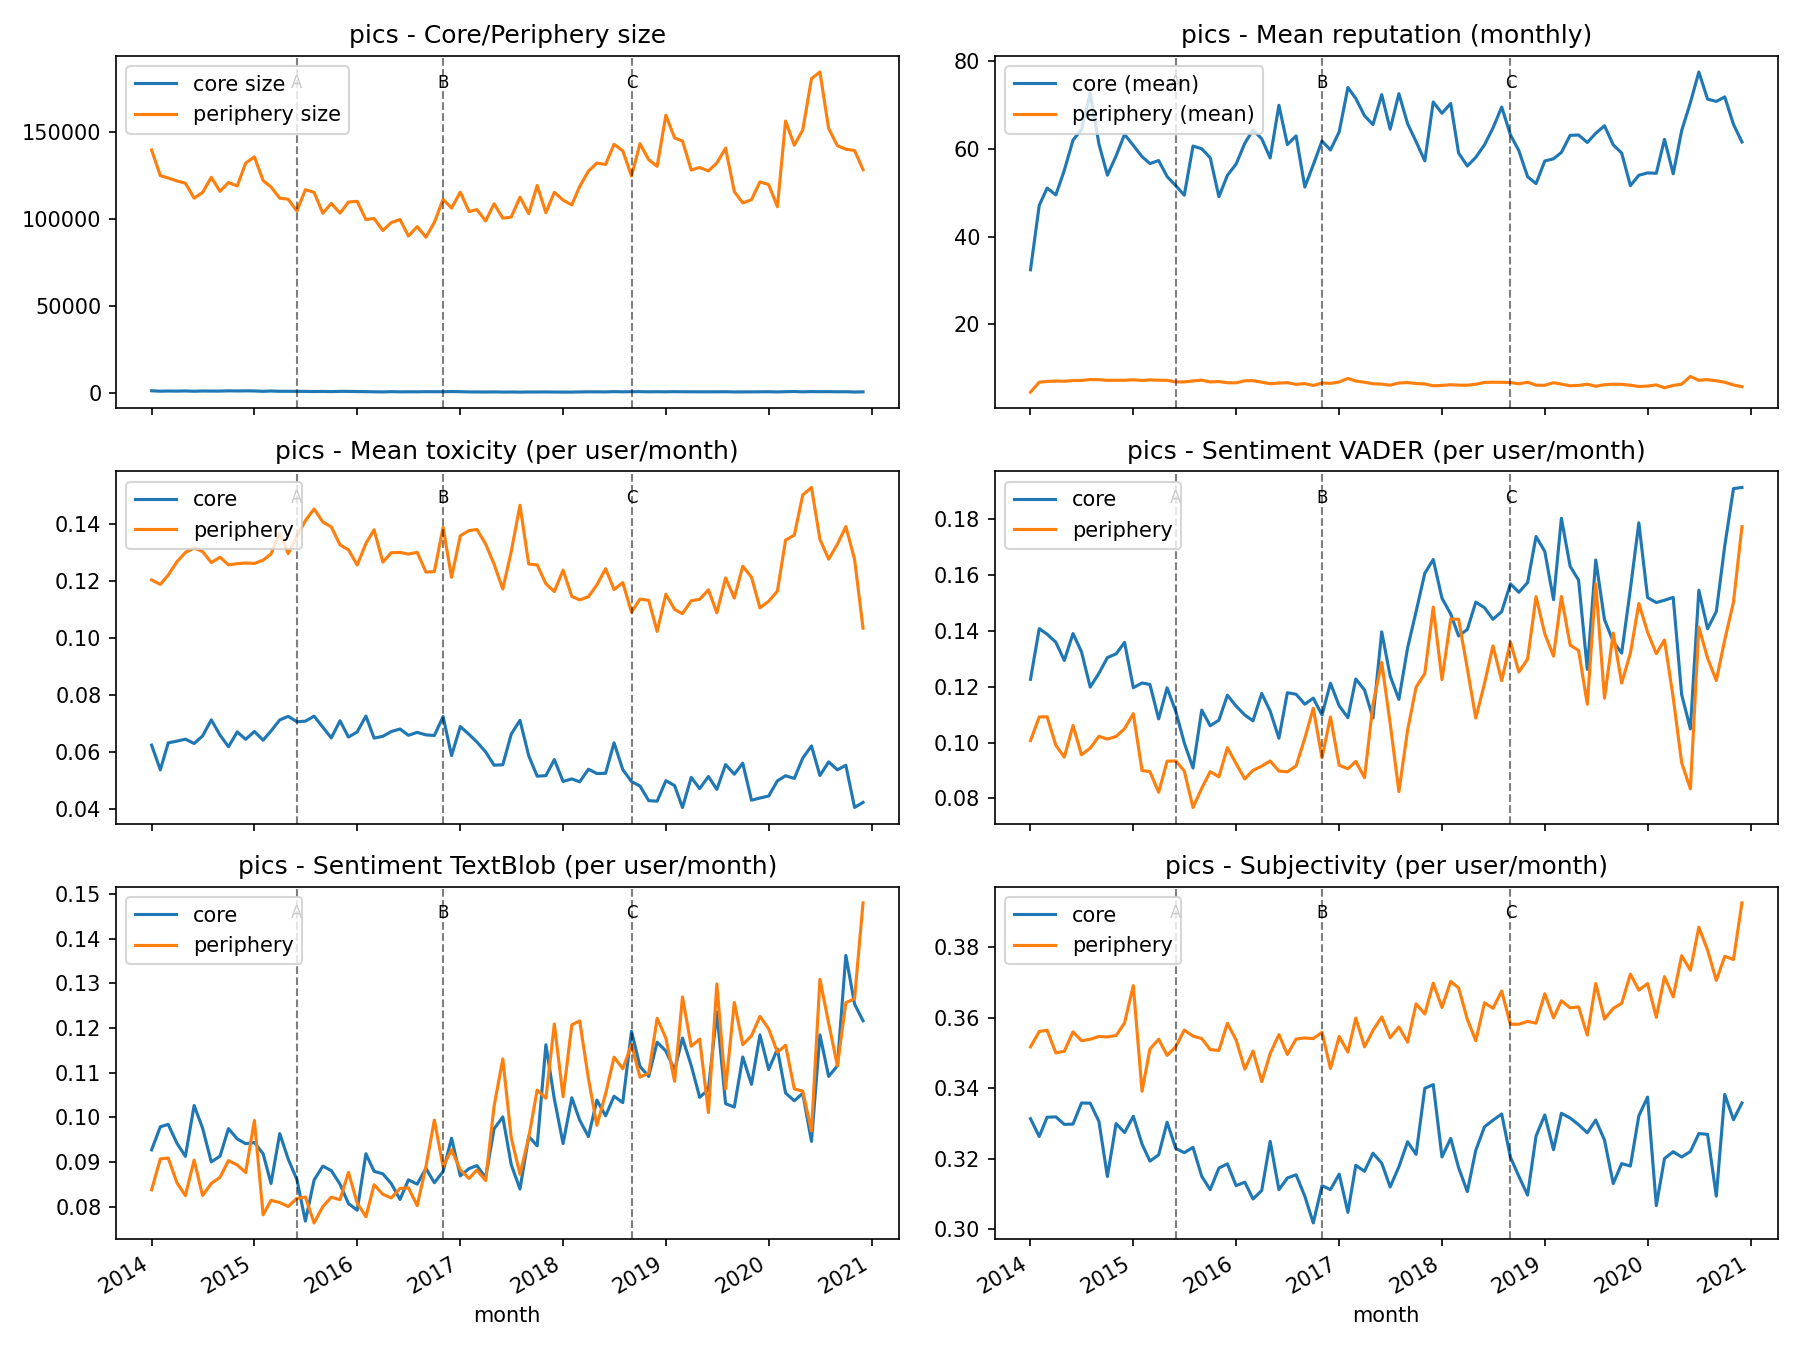
\includegraphics[width=\textwidth]{results/core-periphery/reddit/figures/reddit_pics_cp_panels_2col.png}
\end{frame}

\begin{frame}{Key Insights: Pics - Reddit}
\begin{itemize}
    \item \textbf{Volatile periphery, steady core}: Periphery fluctuates 100K-180K with spike at Event C while core stays flat ($\sim$3K), showing mainstream appeal with stable veteran contributor base
    \item \textbf{Shrinking toxicity gap}: Core maintains lower toxicity (0.04-0.07) than periphery (0.10-0.15) throughout, but gap narrows as both decline—suggesting platform-wide norm shifts
    \item \textbf{Sentiment convergence with role reversal}: Initially periphery more positive, but by 2018 core surpasses periphery (0.14-0.18 vs 0.10-0.15), indicating veteran users became more emotionally invested over time
\end{itemize}
\end{frame}

% -------------------------------------------------------------------
% Technology - Reddit
% -------------------------------------------------------------------
\begin{frame}{Technology - Reddit}
\centering
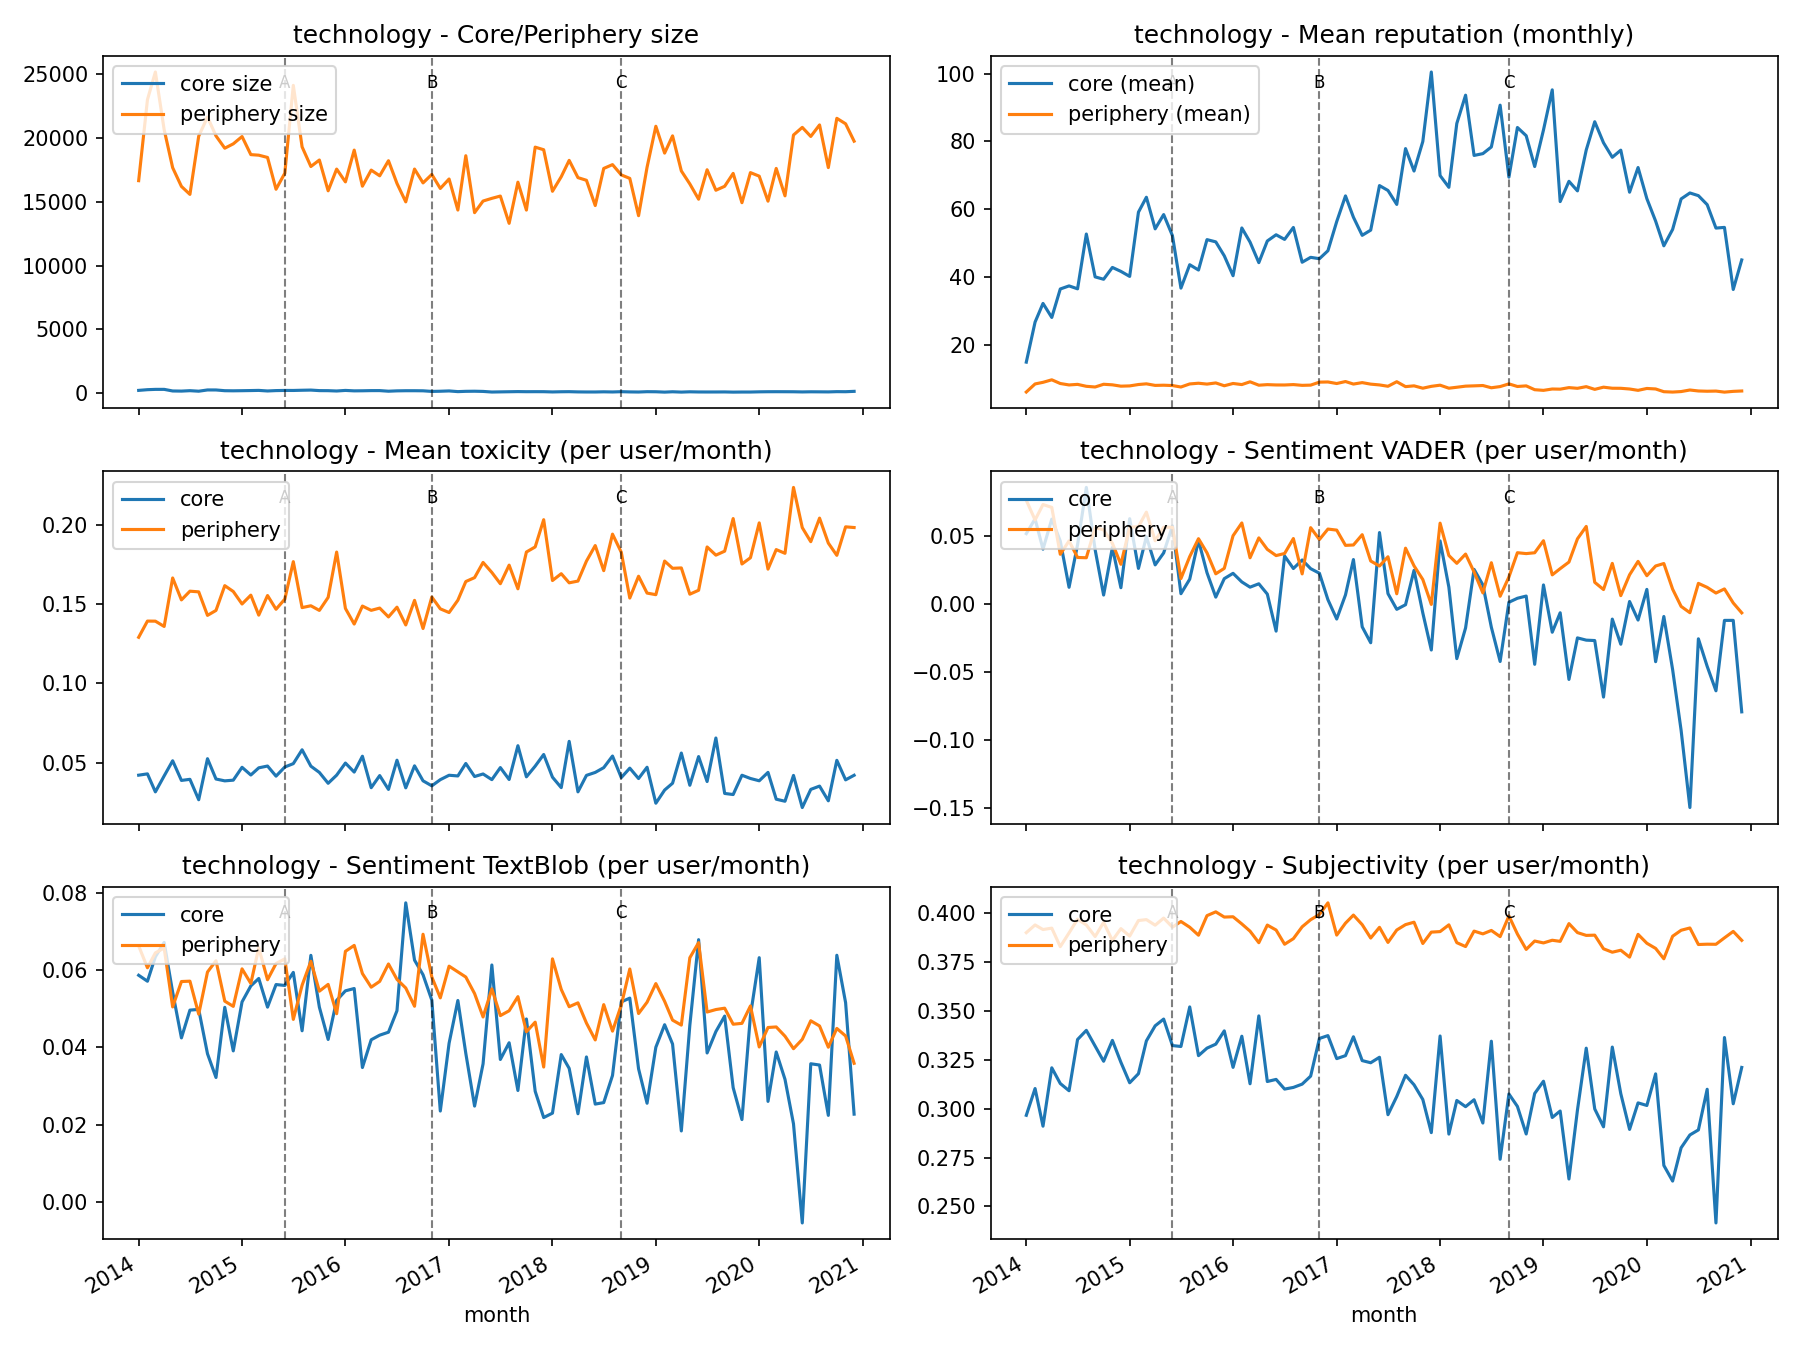
\includegraphics[width=\textwidth]{results/core-periphery/reddit/figures/reddit_technology_cp_panels_2col.png}
\end{frame}

\begin{frame}{Key Insights: Technology - Reddit}
\begin{itemize}
    \item \textbf{Exceptional core reputation growth}: Core reputation climbs from 20 to 100 by Event C (highest growth among all communities), suggesting r/technology successfully retained and elevated expert contributors through moderation crises
    \item \textbf{Extreme toxicity disparity}: Periphery toxicity (0.15-0.22) consistently 3-4x higher than core (0.03-0.05), indicating strong gatekeeping by technical experts against low-quality/inflammatory posts
    \item \textbf{Parallel sentiment decline}: Both core and periphery trend negative post-2017, converging around -0.05 to -0.10, reflecting broader tech industry disillusionment (privacy, monopolies, misinformation) independent of deplatforming events
\end{itemize}
\end{frame}

% -------------------------------------------------------------------
% Videos - Reddit
% -------------------------------------------------------------------
\begin{frame}{Videos - Reddit}
\centering
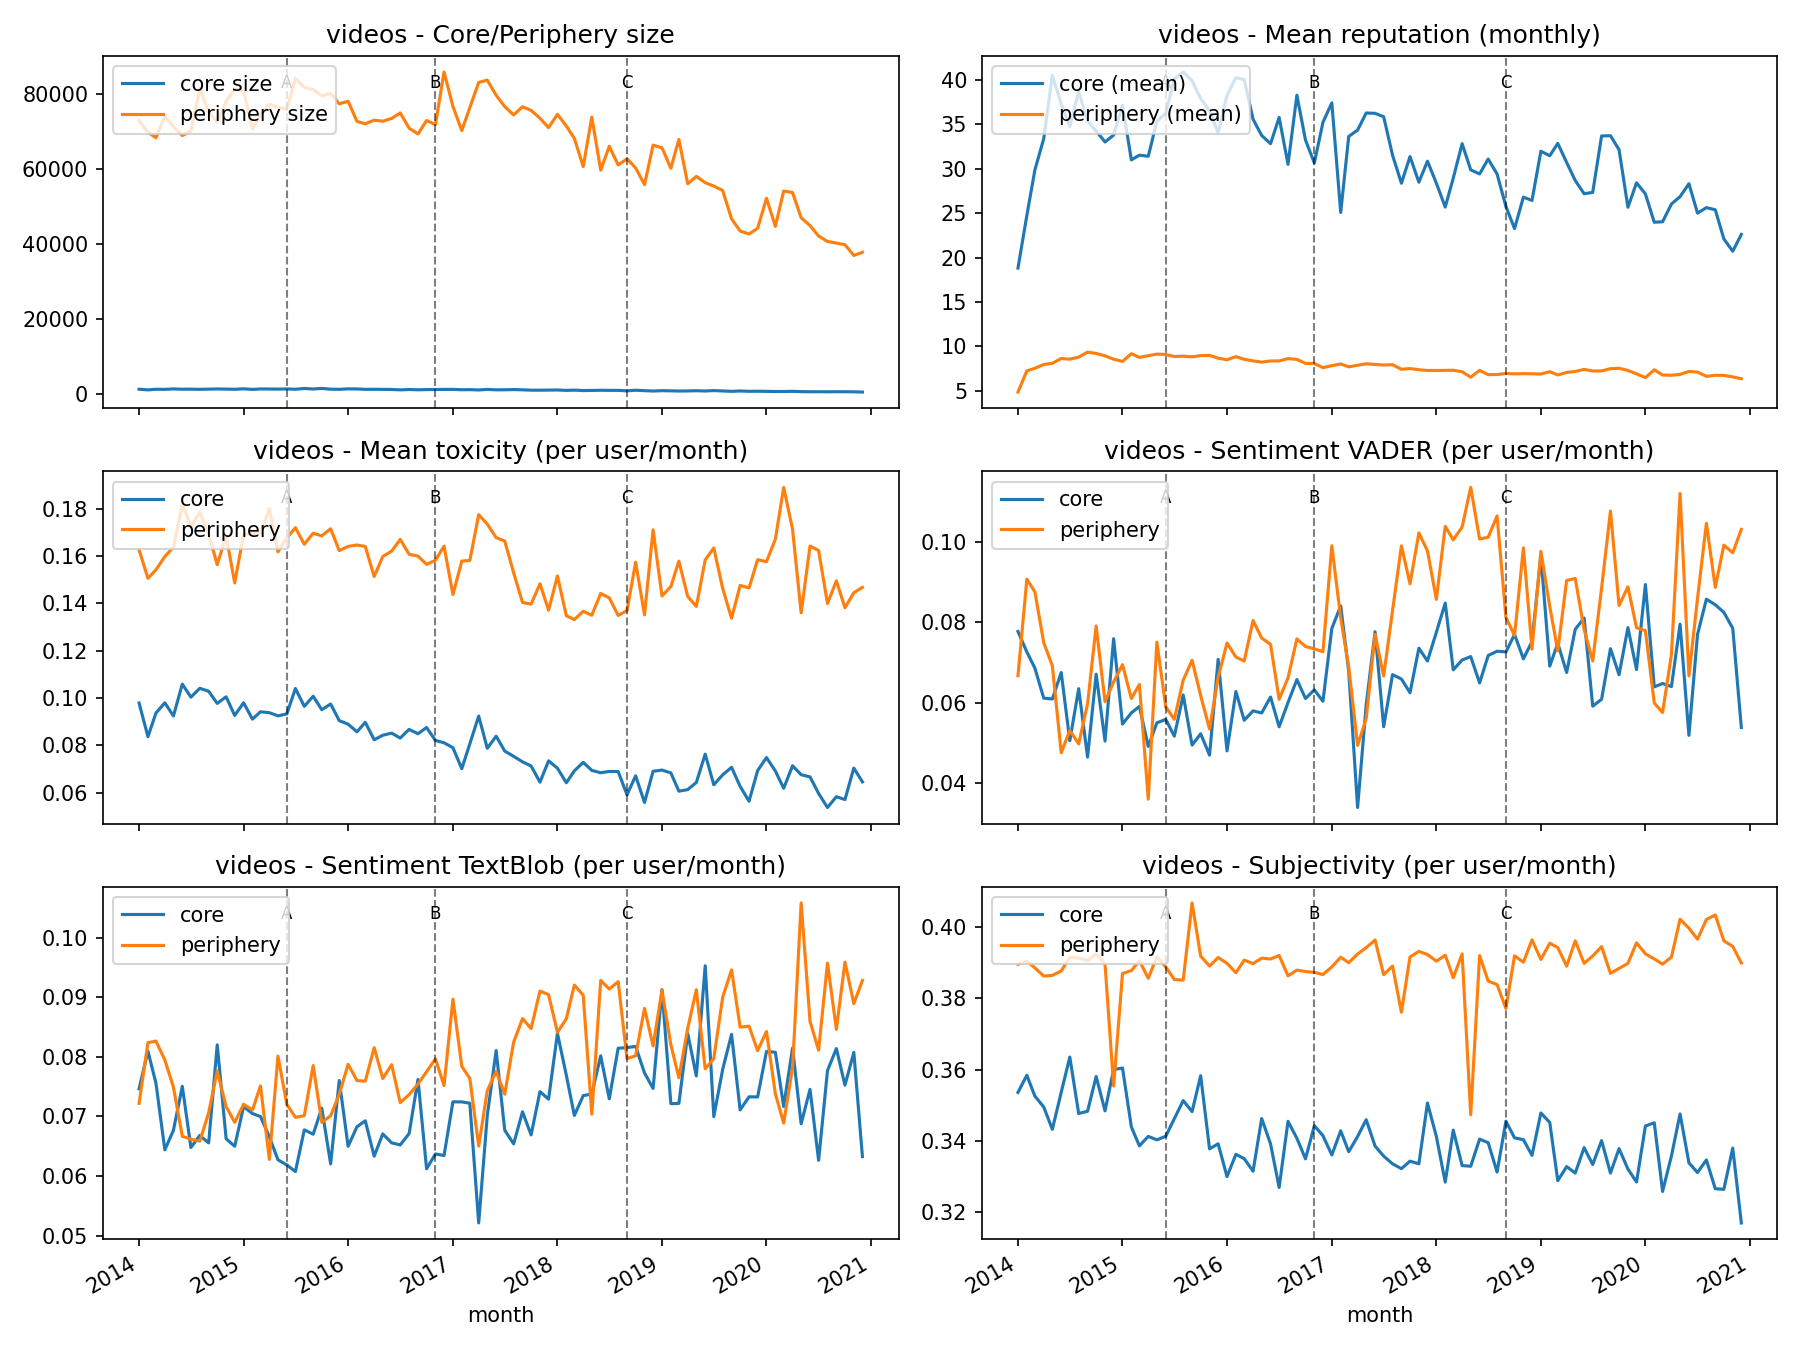
\includegraphics[width=\textwidth]{results/core-periphery/reddit/figures/reddit_videos_cp_panels_2col.png}
\end{frame}

\begin{frame}{Key Insights: Videos - Reddit}
\begin{itemize}
    \item \textbf{Steady decline across metrics}: Periphery shrinks from 80K to 40K (2014-2021) while core flatlines, with core reputation falling from 35 to 20—suggesting r/videos lost appeal as specialized video platforms (YouTube, TikTok) dominated
    \item \textbf{Persistent but declining toxicity gap}: Core maintains lower toxicity (0.06-0.10) than periphery (0.14-0.18), both declining over time as inflammatory content migrated to video platforms
    \item \textbf{Sentiment convergence}: Core and periphery converge around 0.07-0.09 by 2018, losing earlier distinction—indicates homogenization as engaged users left for other platforms
\end{itemize}
\end{frame}

% ===================================================================
% SECTION: Core-Periphery Analysis: Voat
% ===================================================================
\section{Core-Periphery Analysis: Voat}

% -------------------------------------------------------------------
% CringeAnarchy - Voat
% -------------------------------------------------------------------
\begin{frame}{CringeAnarchy - Voat}
\centering
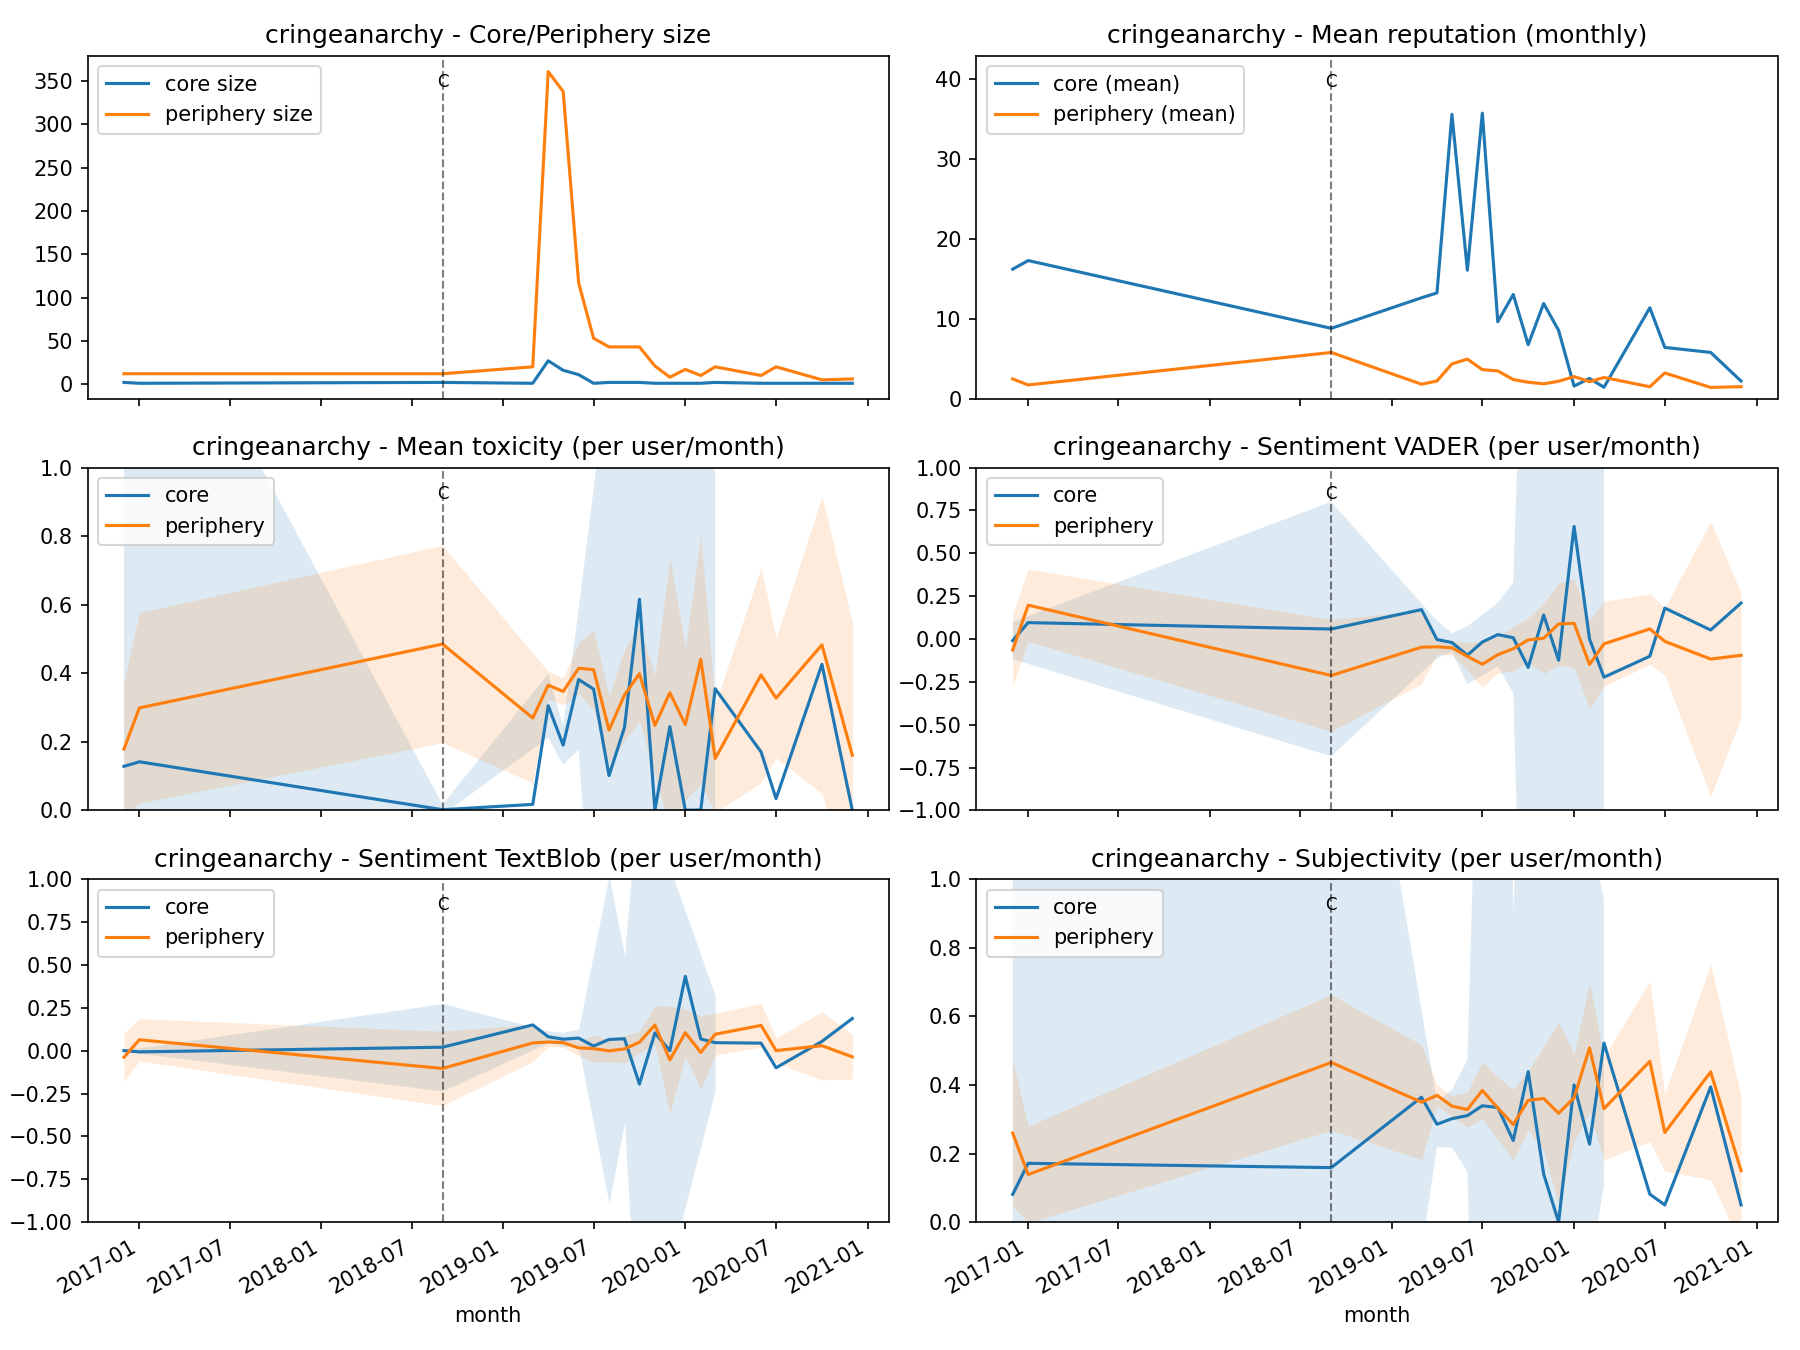
\includegraphics[width=\textwidth]{results/core-periphery/voat/figures/voat_cringeanarchy_cp_panels_2col.png}
\end{frame}

\begin{frame}{Key Insights: CringeAnarchy - Voat}
\begin{itemize}
    \item \textbf{Event C migration spike and collapse}: Periphery explodes to 350 users at 2018 QAnon ban, then crashes to $<$50—CringeAnarchy migrants briefly activated this hate-focused subverse before abandoning it
    \item \textbf{Extreme toxicity oscillations}: Post-migration, toxicity fluctuates wildly (0.0-0.6 for core, 0.2-0.5 for periphery), with core spikes at 0.6—reflects small, volatile user base engaging in extreme content
    \item \textbf{Core reputation anomaly}: Core reputation spikes to 35 at Event C then crashes—suggests brief influx of higher-status migrants who quickly churned out, leaving low-reputation remnant
\end{itemize}
\end{frame}

% -------------------------------------------------------------------
% FatPeopleHate - Voat
% -------------------------------------------------------------------
\begin{frame}{FatPeopleHate - Voat}
\centering
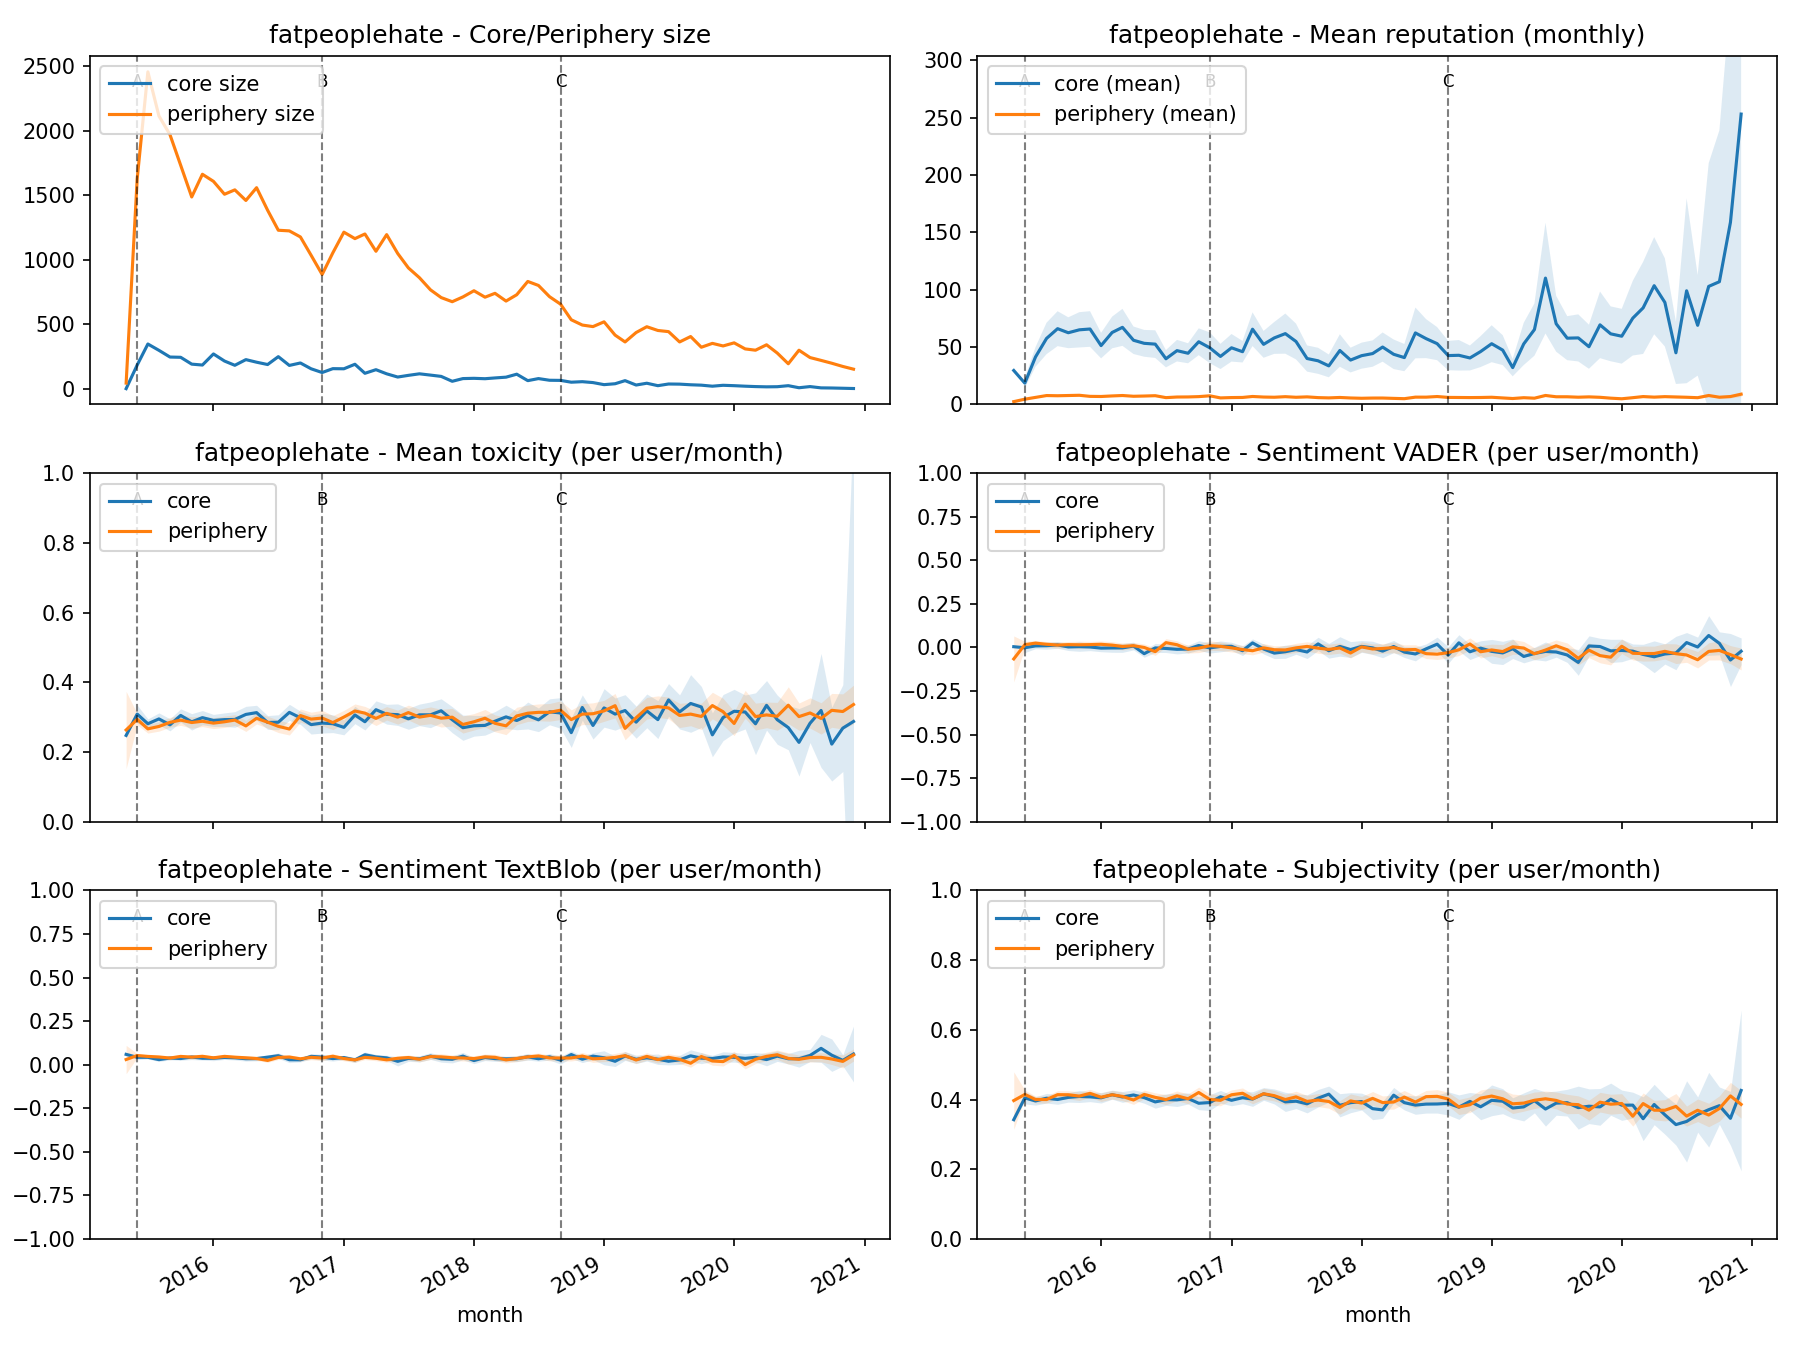
\includegraphics[width=\textwidth]{results/core-periphery/voat/figures/voat_fatpeoplehate_cp_panels_2col.png}
\end{frame}

\begin{frame}{Key Insights: FatPeopleHate - Voat}
\begin{itemize}
    \item \textbf{Sustained but declining activity}: Periphery starts at 2000 (largest Voat community post-Event A) and gradually declines to 200 by 2021, while core stabilizes at 300-400—original r/fatpeoplehate migrants maintained long-term presence
    \item \textbf{Consistently high toxicity}: Both core and periphery maintain 0.28-0.34 toxicity (3-4x typical Reddit levels) throughout entire timeline, with convergence—hate speech remained normalized community norm
    \item \textbf{Late reputation surge}: Core reputation spikes to 250 in 2021 (near platform shutdown), possibly reflecting measurement artifact or final concentration of die-hard users accumulating karma
\end{itemize}
\end{frame}

% -------------------------------------------------------------------
% Funny - Voat
% -------------------------------------------------------------------
\begin{frame}{Funny - Voat}
\centering
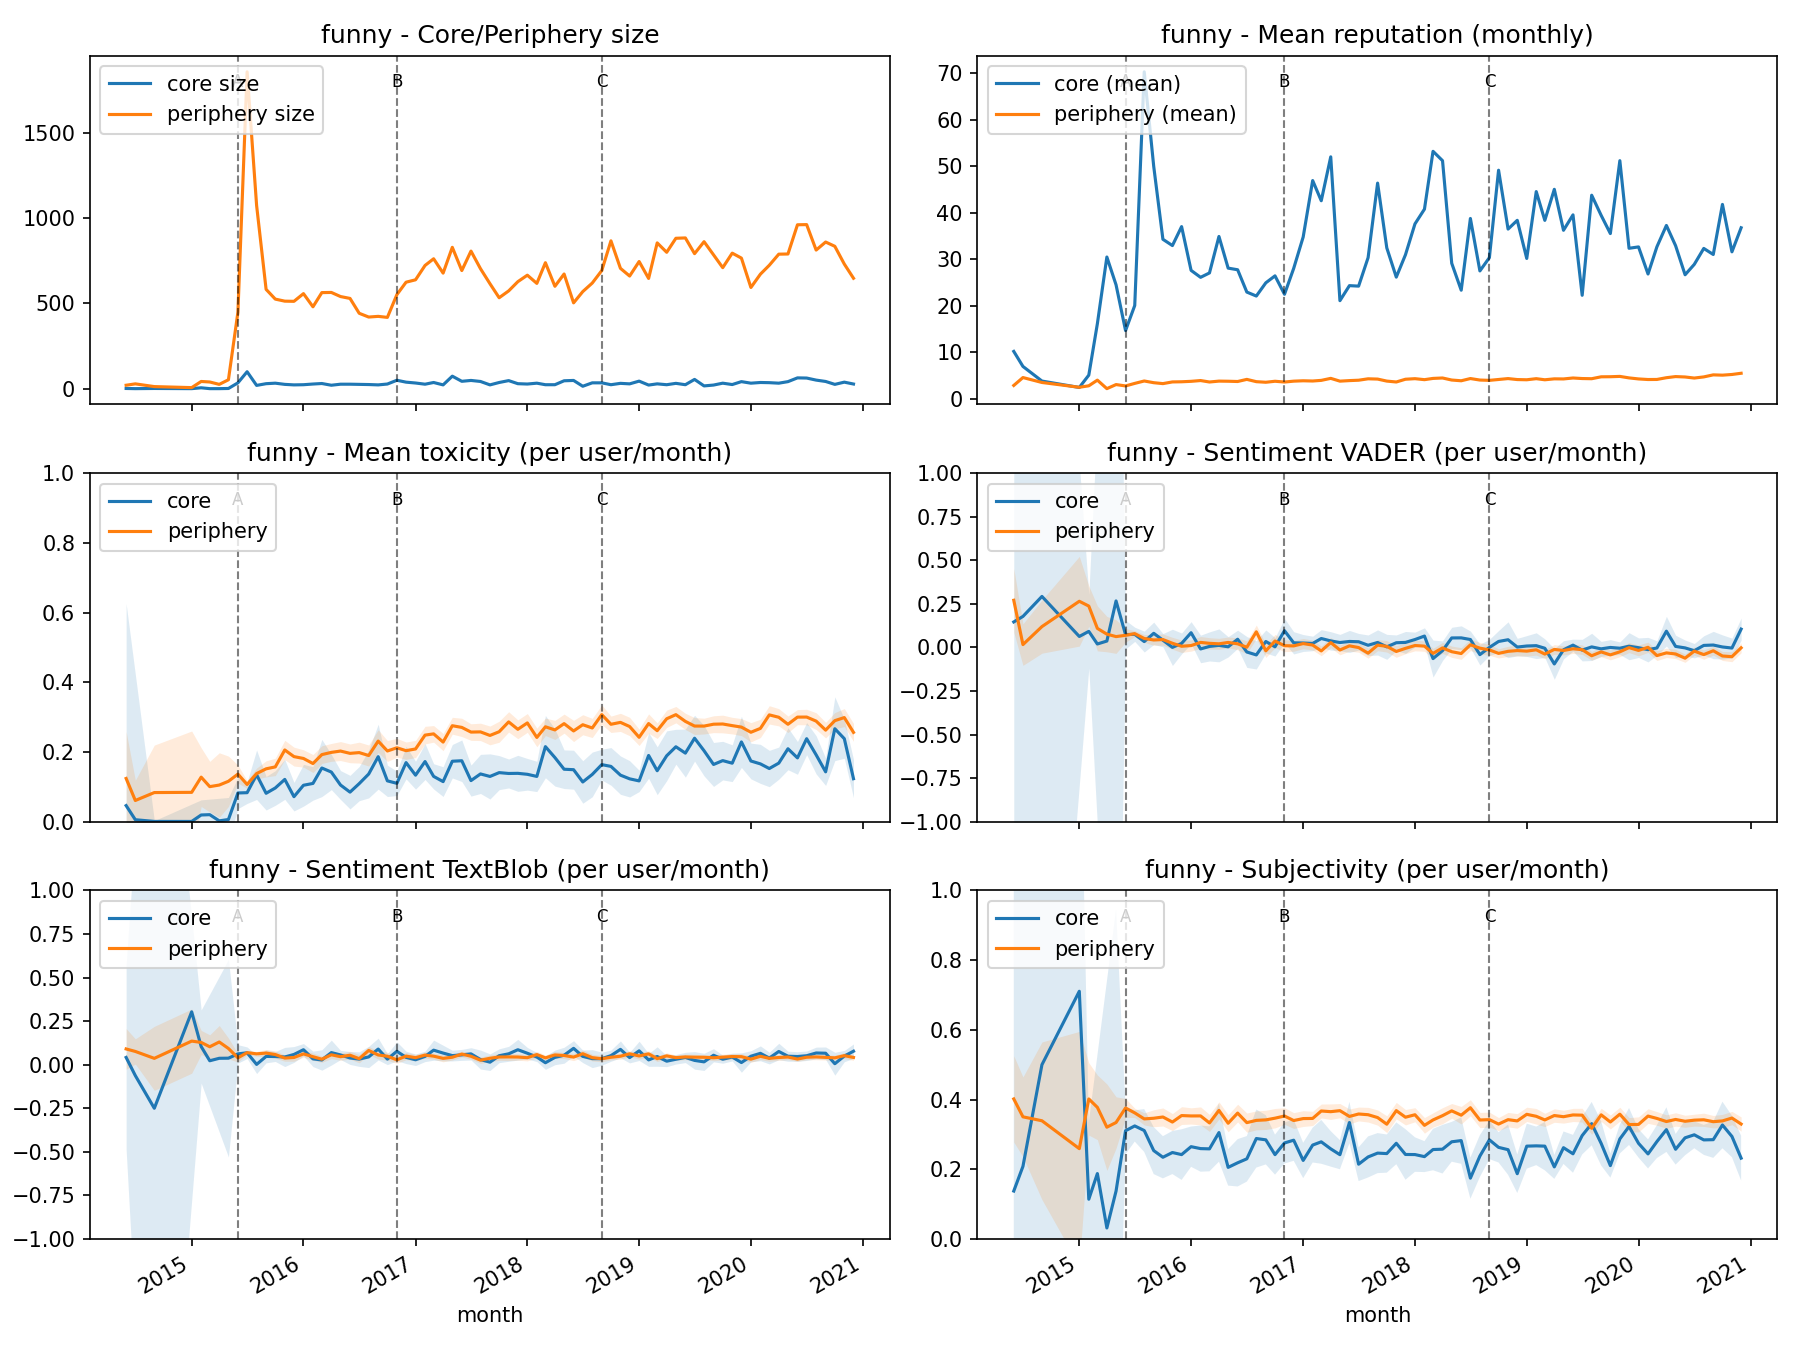
\includegraphics[width=\textwidth]{results/core-periphery/voat/figures/voat_funny_cp_panels_2col.png}
\end{frame}

\begin{frame}{Key Insights: Funny - Voat}
\begin{itemize}
    \item \textbf{Event A surge then stabilization}: Periphery spikes to 1500 at 2015 harassment ban, then stabilizes at 600-900—v/funny absorbed generalist r/fatpeoplehate migrants seeking entertainment but retained substantial base
    \item \textbf{Escalating toxicity divergence}: Periphery toxicity climbs from 0.12 to 0.30 (2015-2021) while core rises from 0.08 to 0.25—both groups radicalized over time as platform culture shifted
    \item \textbf{Sentiment collapse}: Both core and periphery drop from positive (0.05-0.20) to near-zero/negative by 2017, never recovering—entertainment content became increasingly cynical and hostile
\end{itemize}
\end{frame}

% -------------------------------------------------------------------
% Gaming - Voat
% -------------------------------------------------------------------
\begin{frame}{Gaming - Voat}
\centering
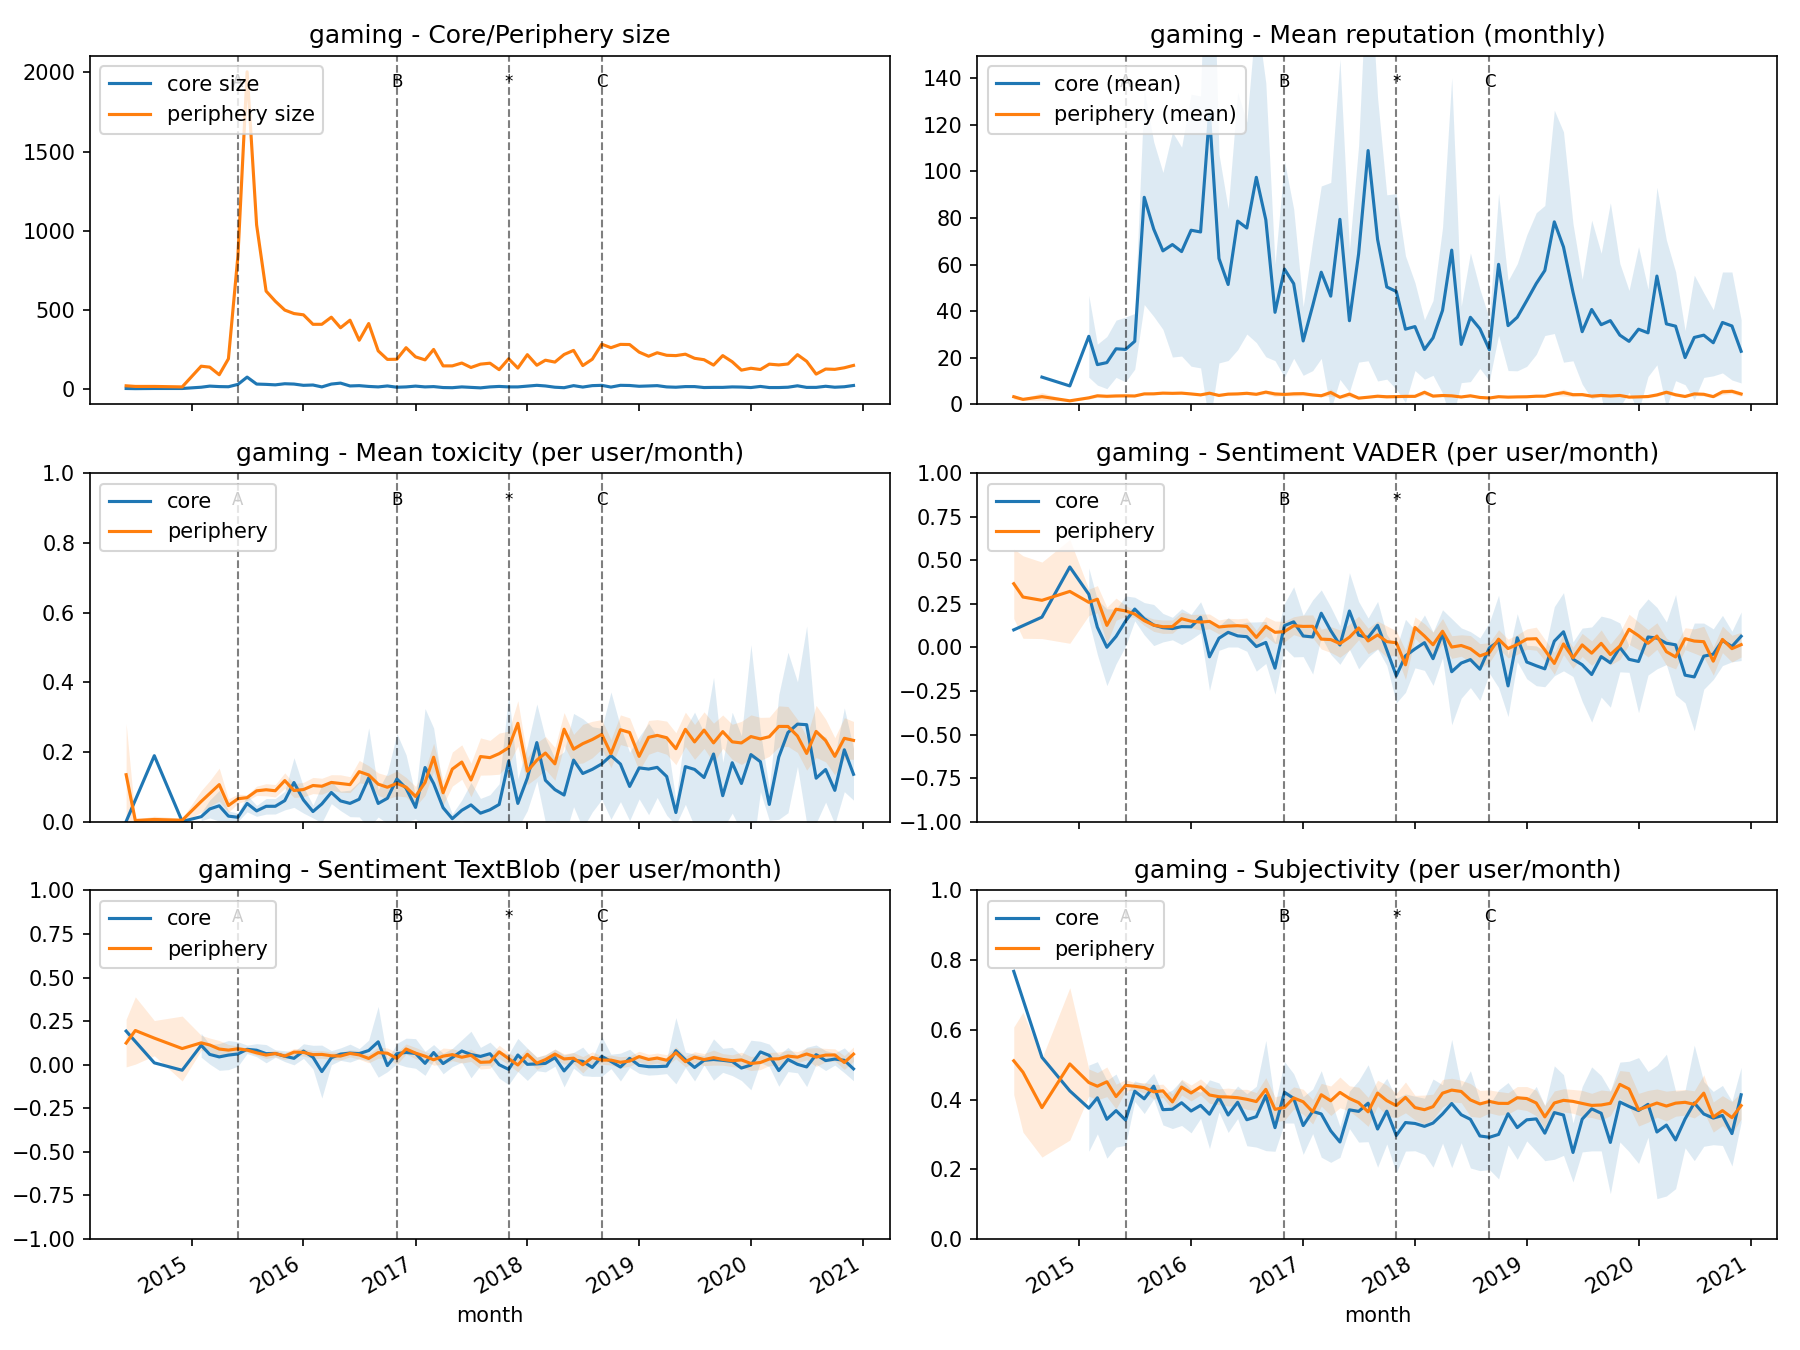
\includegraphics[width=\textwidth]{results/core-periphery/voat/figures/voat_gaming_cp_panels_2col.png}
\end{frame}

\begin{frame}{Key Insights: Gaming - Voat}
\begin{itemize}
    \item \textbf{Boom-bust cycle at Event A}: Periphery surges to 1800 (2015 ban), crashes to 200, then flatlines at 100—initial r/fatpeoplehate migrants briefly tried v/gaming but abandoned it as conspiracy users dominated Voat
    \item \textbf{Core reputation volatility}: Core reputation oscillates wildly (20-110), peaking around Events B/C, then declining—small core couldn't stabilize as generalist migrants churned out
    \item \textbf{Converging negative sentiment}: Both groups trend from positive (0.20-0.30) in 2015 to near-zero/negative by 2020—gaming discussions became increasingly pessimistic as community fragmented
\end{itemize}
\end{frame}

% -------------------------------------------------------------------
% Gifs - Voat
% -------------------------------------------------------------------
\begin{frame}{Gifs - Voat}
\centering
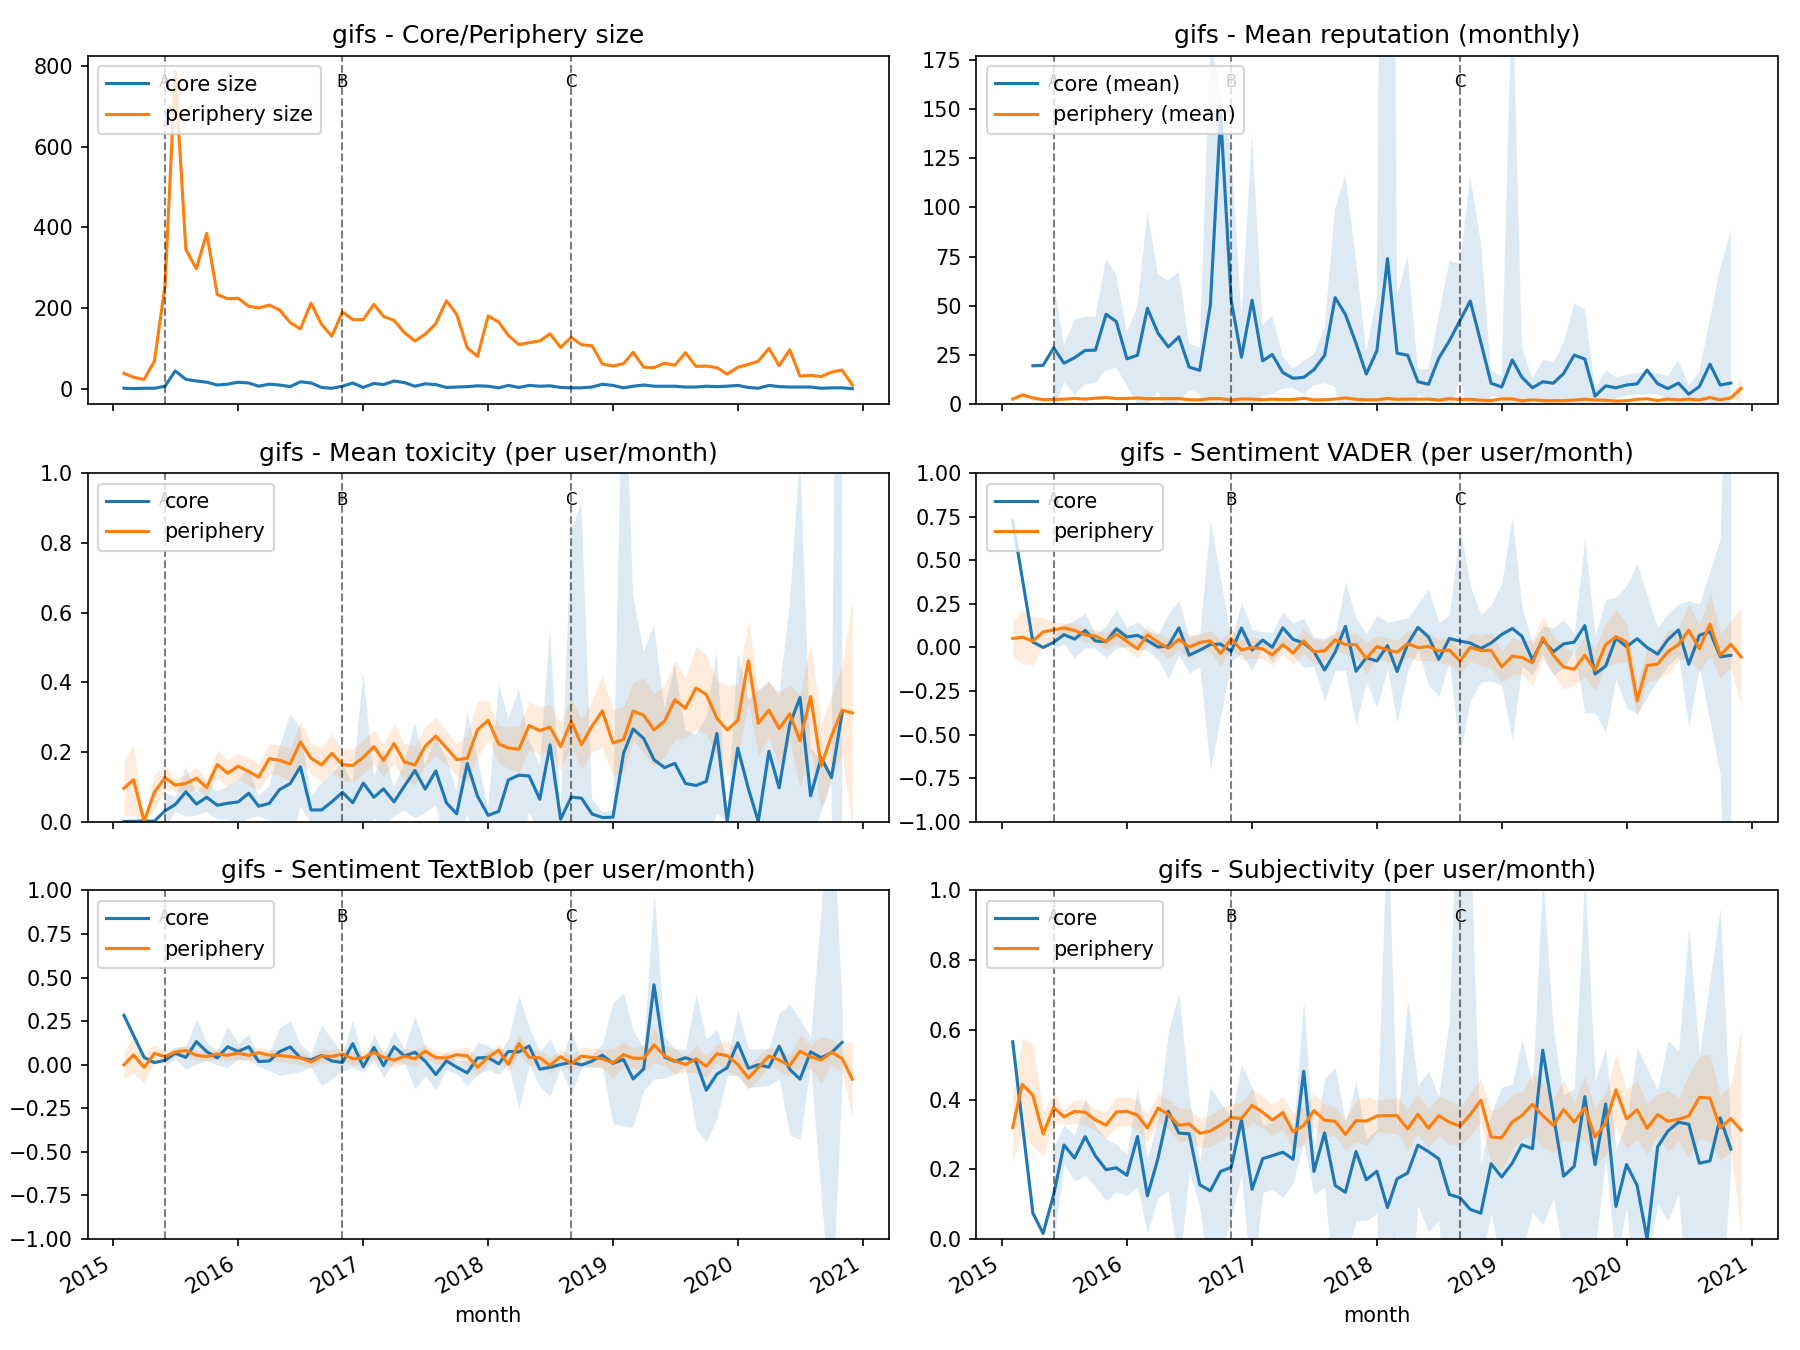
\includegraphics[width=\textwidth]{results/core-periphery/voat/figures/voat_gifs_cp_panels_2col.png}
\end{frame}

\begin{frame}{Key Insights: Gifs - Voat}
\begin{itemize}
    \item \textbf{Event A spike then gradual decline}: Periphery peaks at 650 (2015), steadily declines to $<$100 by 2021—v/gifs couldn't sustain generalist migrants as static gifs lost relevance platform-wide
    \item \textbf{Late toxicity surge}: Periphery toxicity escalates from 0.15 to 0.45 after Event C (2018-2021), suggesting conspiracy-focused late arrivals dominated the dying community
    \item \textbf{Core reputation spike anomaly}: Core reputation jumps to 120-150 around Event B with high volatility—possibly measurement artifact from small sample size ($\sim$20-30 core users)
\end{itemize}
\end{frame}

% -------------------------------------------------------------------
% GreatAwakening - Voat
% -------------------------------------------------------------------
\begin{frame}{GreatAwakening - Voat}
\centering
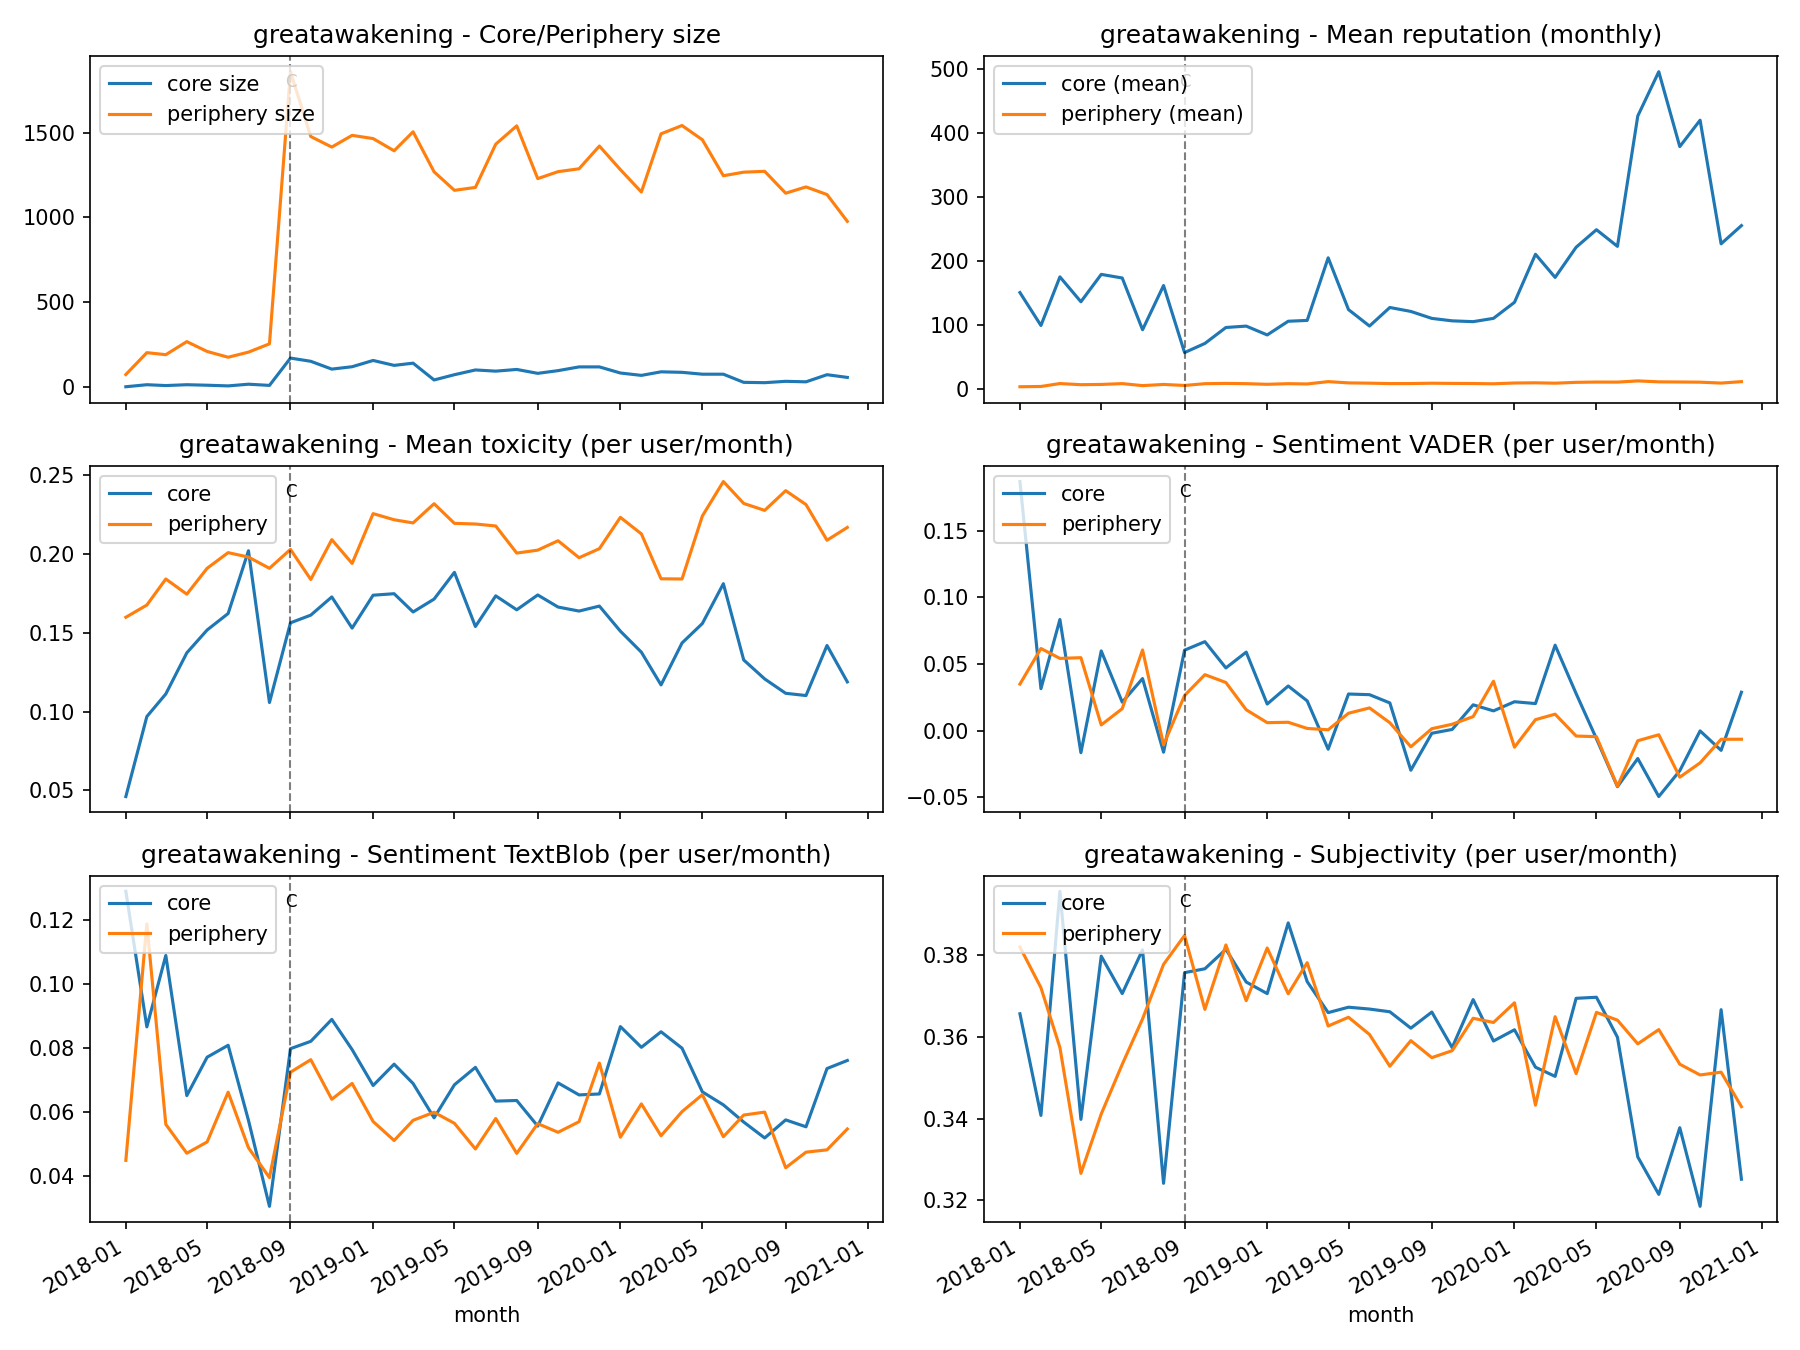
\includegraphics[width=\textwidth]{results/core-periphery/voat/figures/voat_greatawakening_cp_panels_2col.png}
\end{frame}

\begin{frame}{Key Insights: GreatAwakening - Voat}
\begin{itemize}
    \item \textbf{Event C identity-driven migration}: Periphery surges to 1500+ at 2018 QAnon ban and sustains 1100-1500 through 2021—conspiracy narratives tied to user identity created exceptional retention (as predicted by RECRO framework)
    \item \textbf{Core reputation explosion}: Core reputation climbs from 100 to 500 by 2020 (highest across all Voat communities)—QAnon leaders accumulated massive influence within tightly-knit conspiratorial network
    \item \textbf{Moderate toxicity convergence}: Both groups maintain 0.15-0.25 toxicity (lower than hate communities)—conspiracy focus channeled engagement toward narrative-building rather than harassment
\end{itemize}
\end{frame}

% -------------------------------------------------------------------
% KotakuInAction - Voat
% -------------------------------------------------------------------
\begin{frame}{KotakuInAction - Voat}
\centering
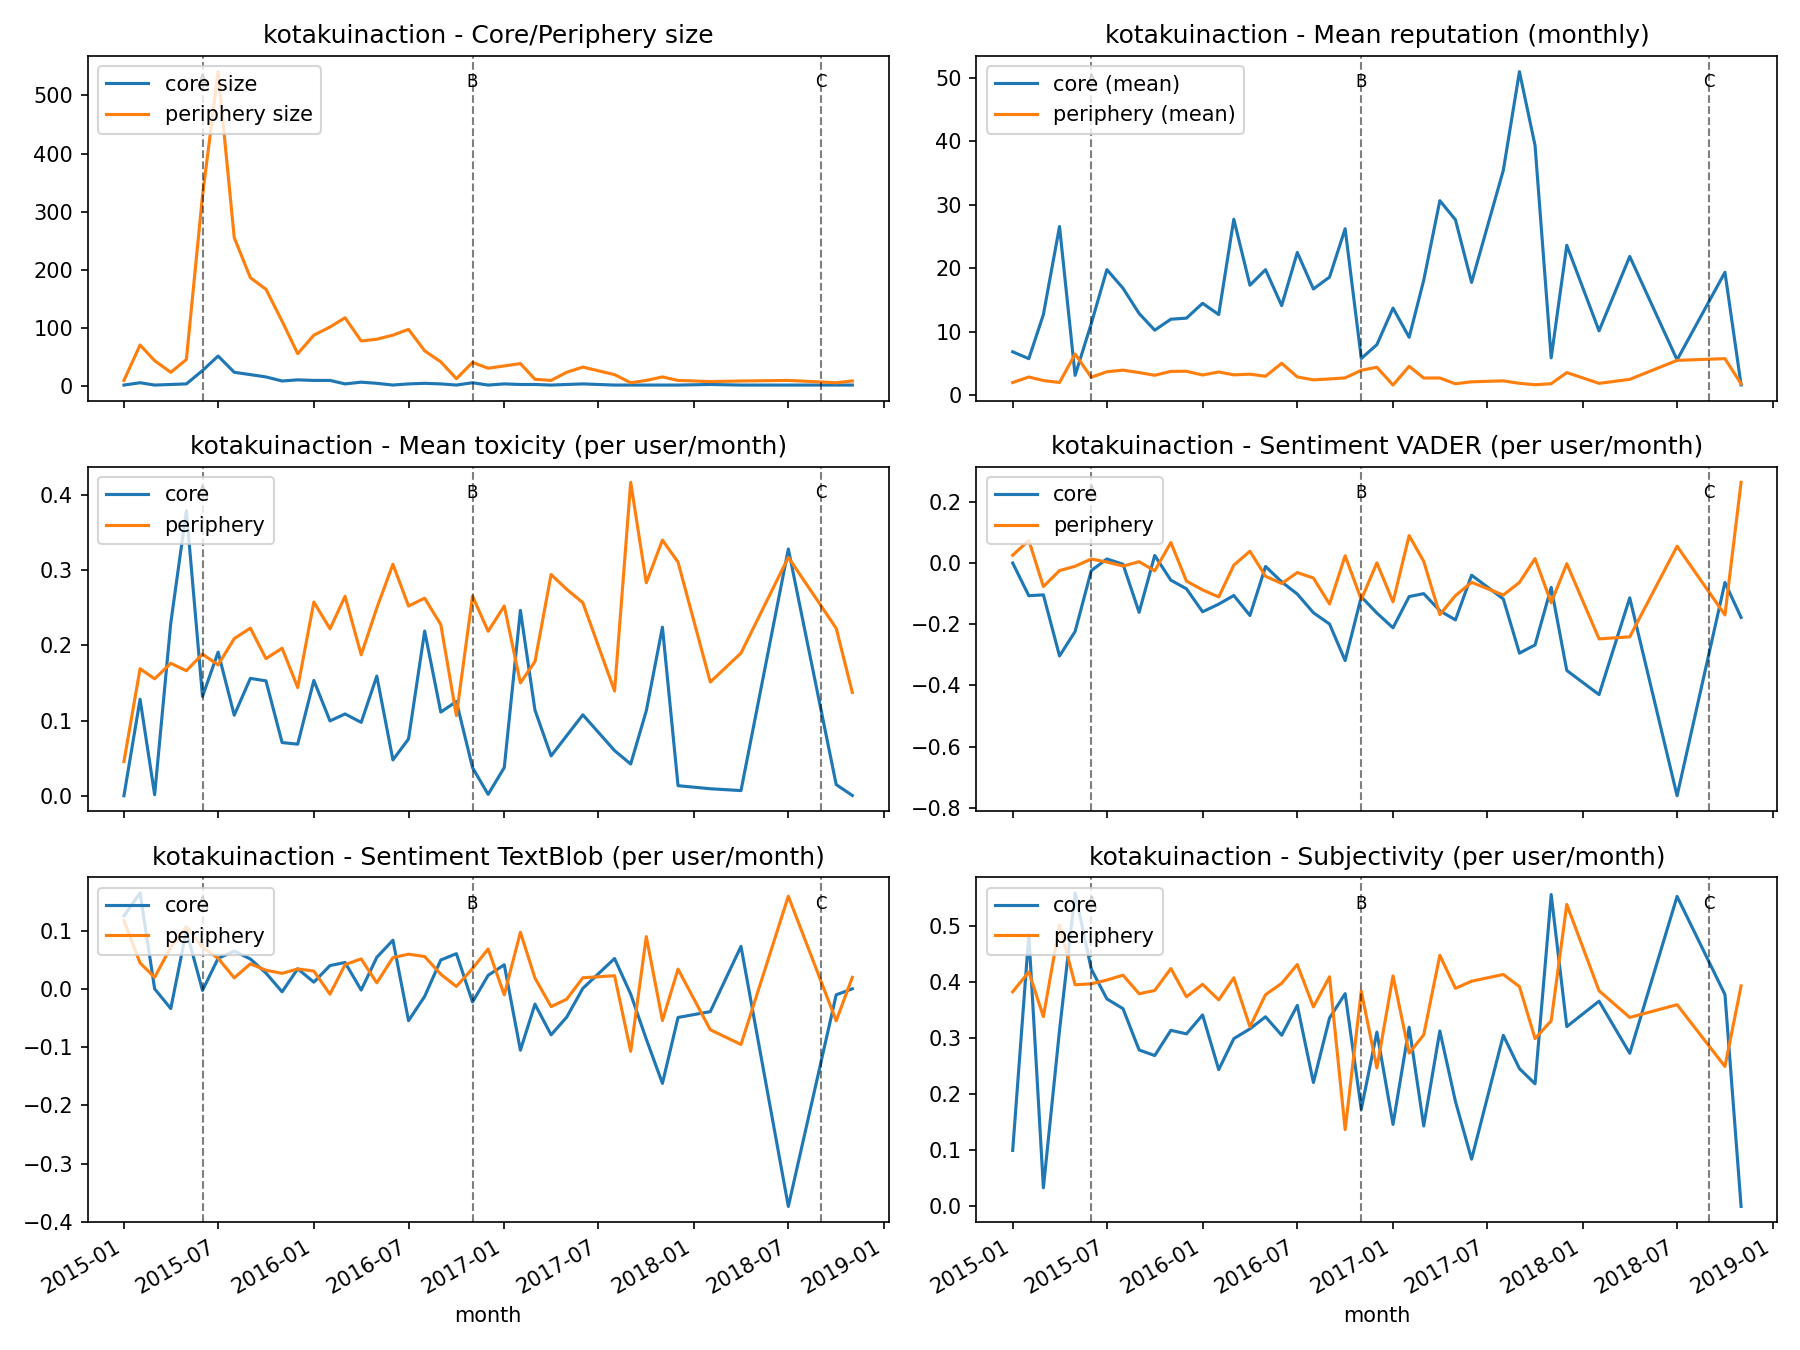
\includegraphics[width=\textwidth]{results/core-periphery/voat/figures/voat_kotakuinaction_cp_panels_2col.png}
\end{frame}

\begin{frame}{Key Insights: KotakuInAction - Voat}
\begin{itemize}
    \item \textbf{Event A spike then rapid abandonment}: Periphery surges to 450 (2015), crashes to $<$50 by 2017—GamerGate-focused users didn't maintain long-term presence, likely staying primarily on Reddit
    \item \textbf{High toxicity with wild fluctuations}: Toxicity oscillates 0.10-0.40 with core spikes at 0.40+, reflecting small, volatile user base engaging in culture-war rhetoric
    \item \textbf{Deeply negative sentiment}: Core sentiment plummets to -0.6 to -0.8 by 2018 (lowest observed)—grievance-driven community became increasingly pessimistic before collapse
\end{itemize}
\end{frame}

% -------------------------------------------------------------------
% MensRights - Voat
% -------------------------------------------------------------------
\begin{frame}{MensRights - Voat}
\centering
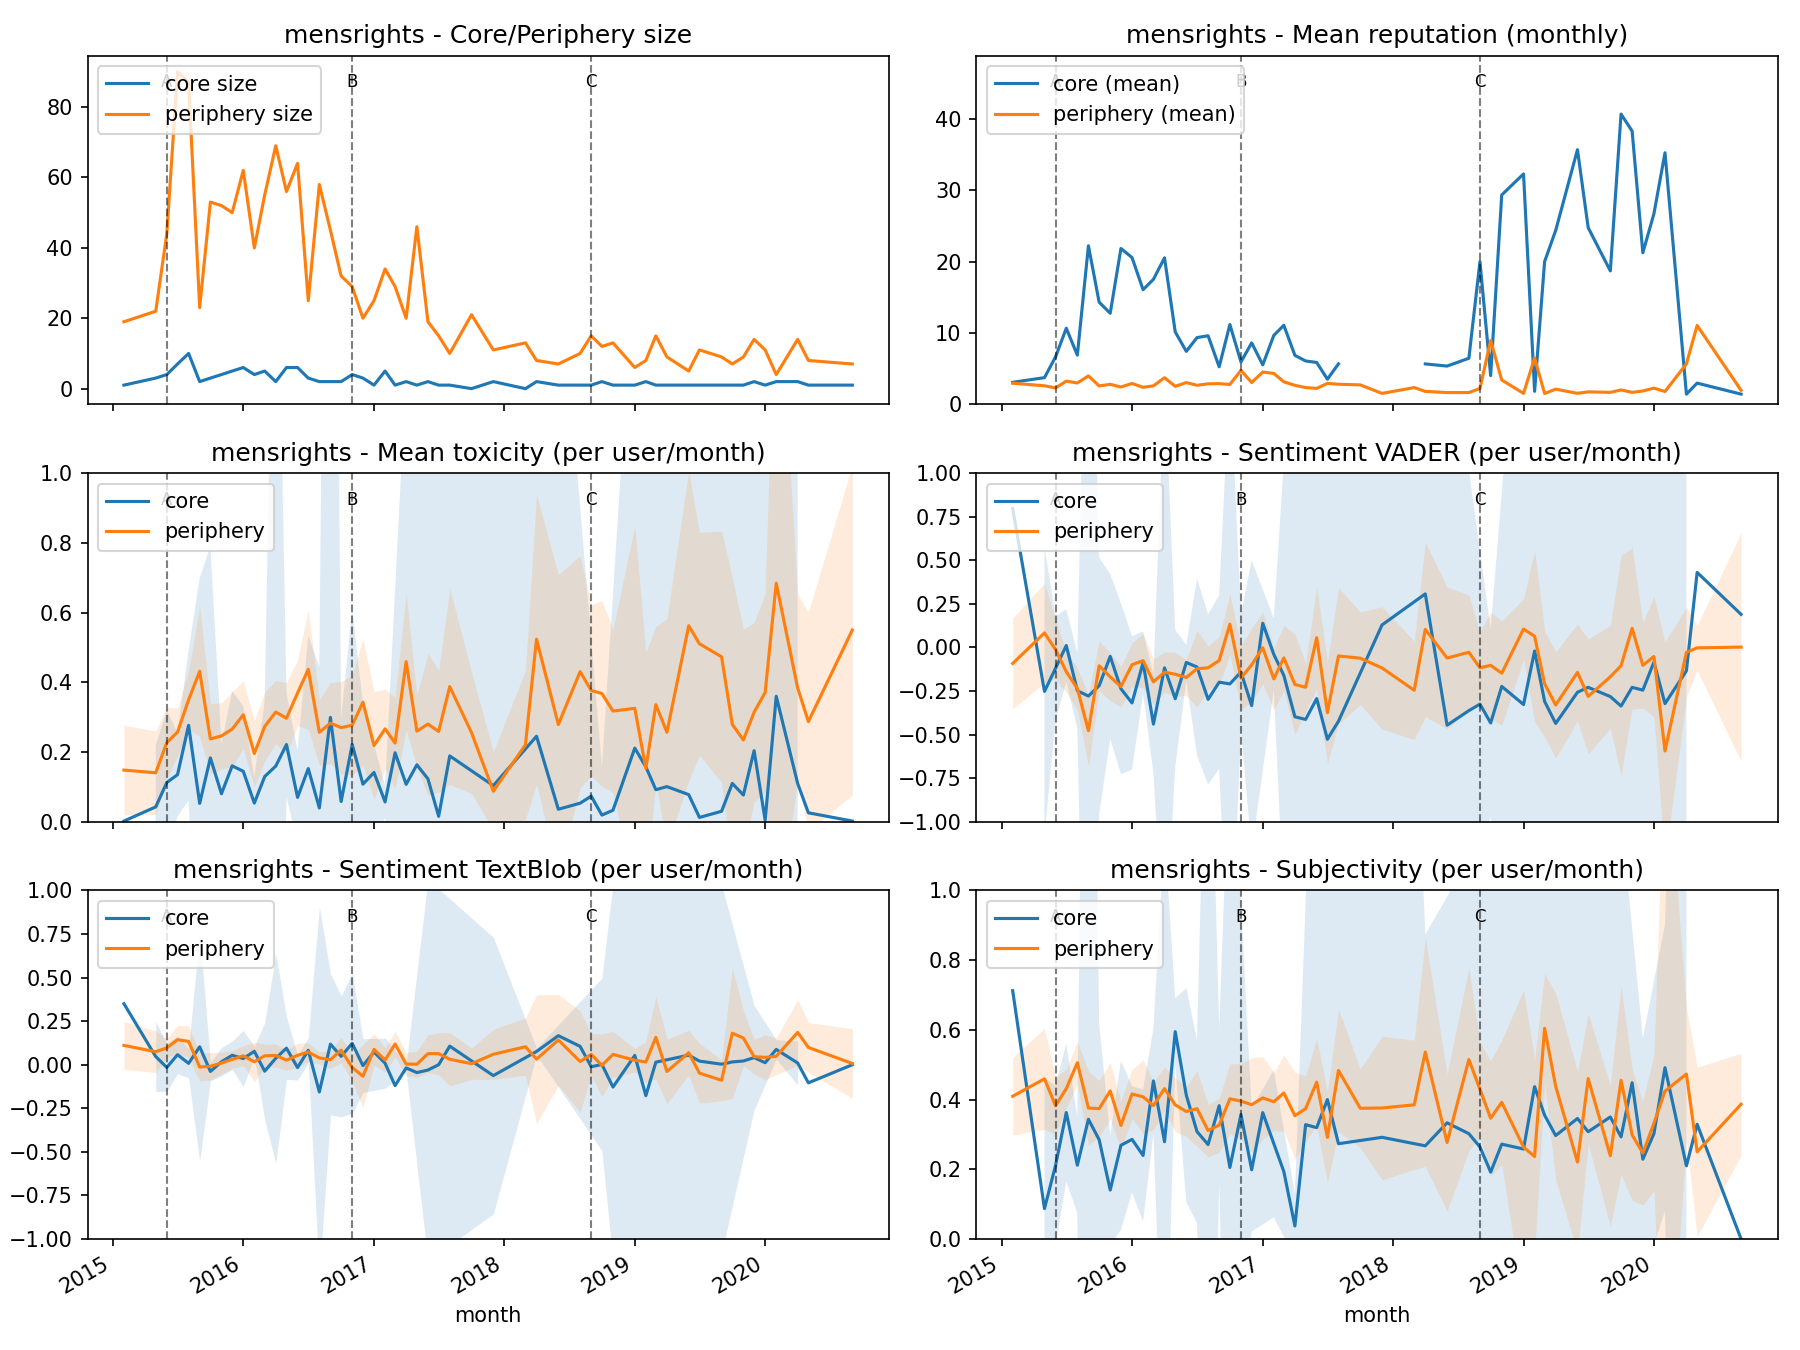
\includegraphics[width=\textwidth]{results/core-periphery/voat/figures/voat_mensrights_cp_panels_2col.png}
\end{frame}

\begin{frame}{Key Insights: MensRights - Voat}
\begin{itemize}
    \item \textbf{Event A spike then gradual decline}: Periphery peaks at 80 (2015), declines to $<$10 by 2020—MensRights migrants didn't establish lasting presence, possibly remaining on more moderate r/MensRights
    \item \textbf{Extreme periphery toxicity}: Periphery toxicity escalates to 0.40-0.70 (highest observed), far exceeding core's 0.10-0.30—small periphery became extremely radicalized
    \item \textbf{Core reputation spikes at Event C}: Core reputation jumps to 35-40 around 2018-2019 with high volatility—reflects small sample artifacts as community neared extinction
\end{itemize}
\end{frame}

% -------------------------------------------------------------------
% MillionDollarExtreme - Voat
% -------------------------------------------------------------------
\begin{frame}{MillionDollarExtreme - Voat}
\centering
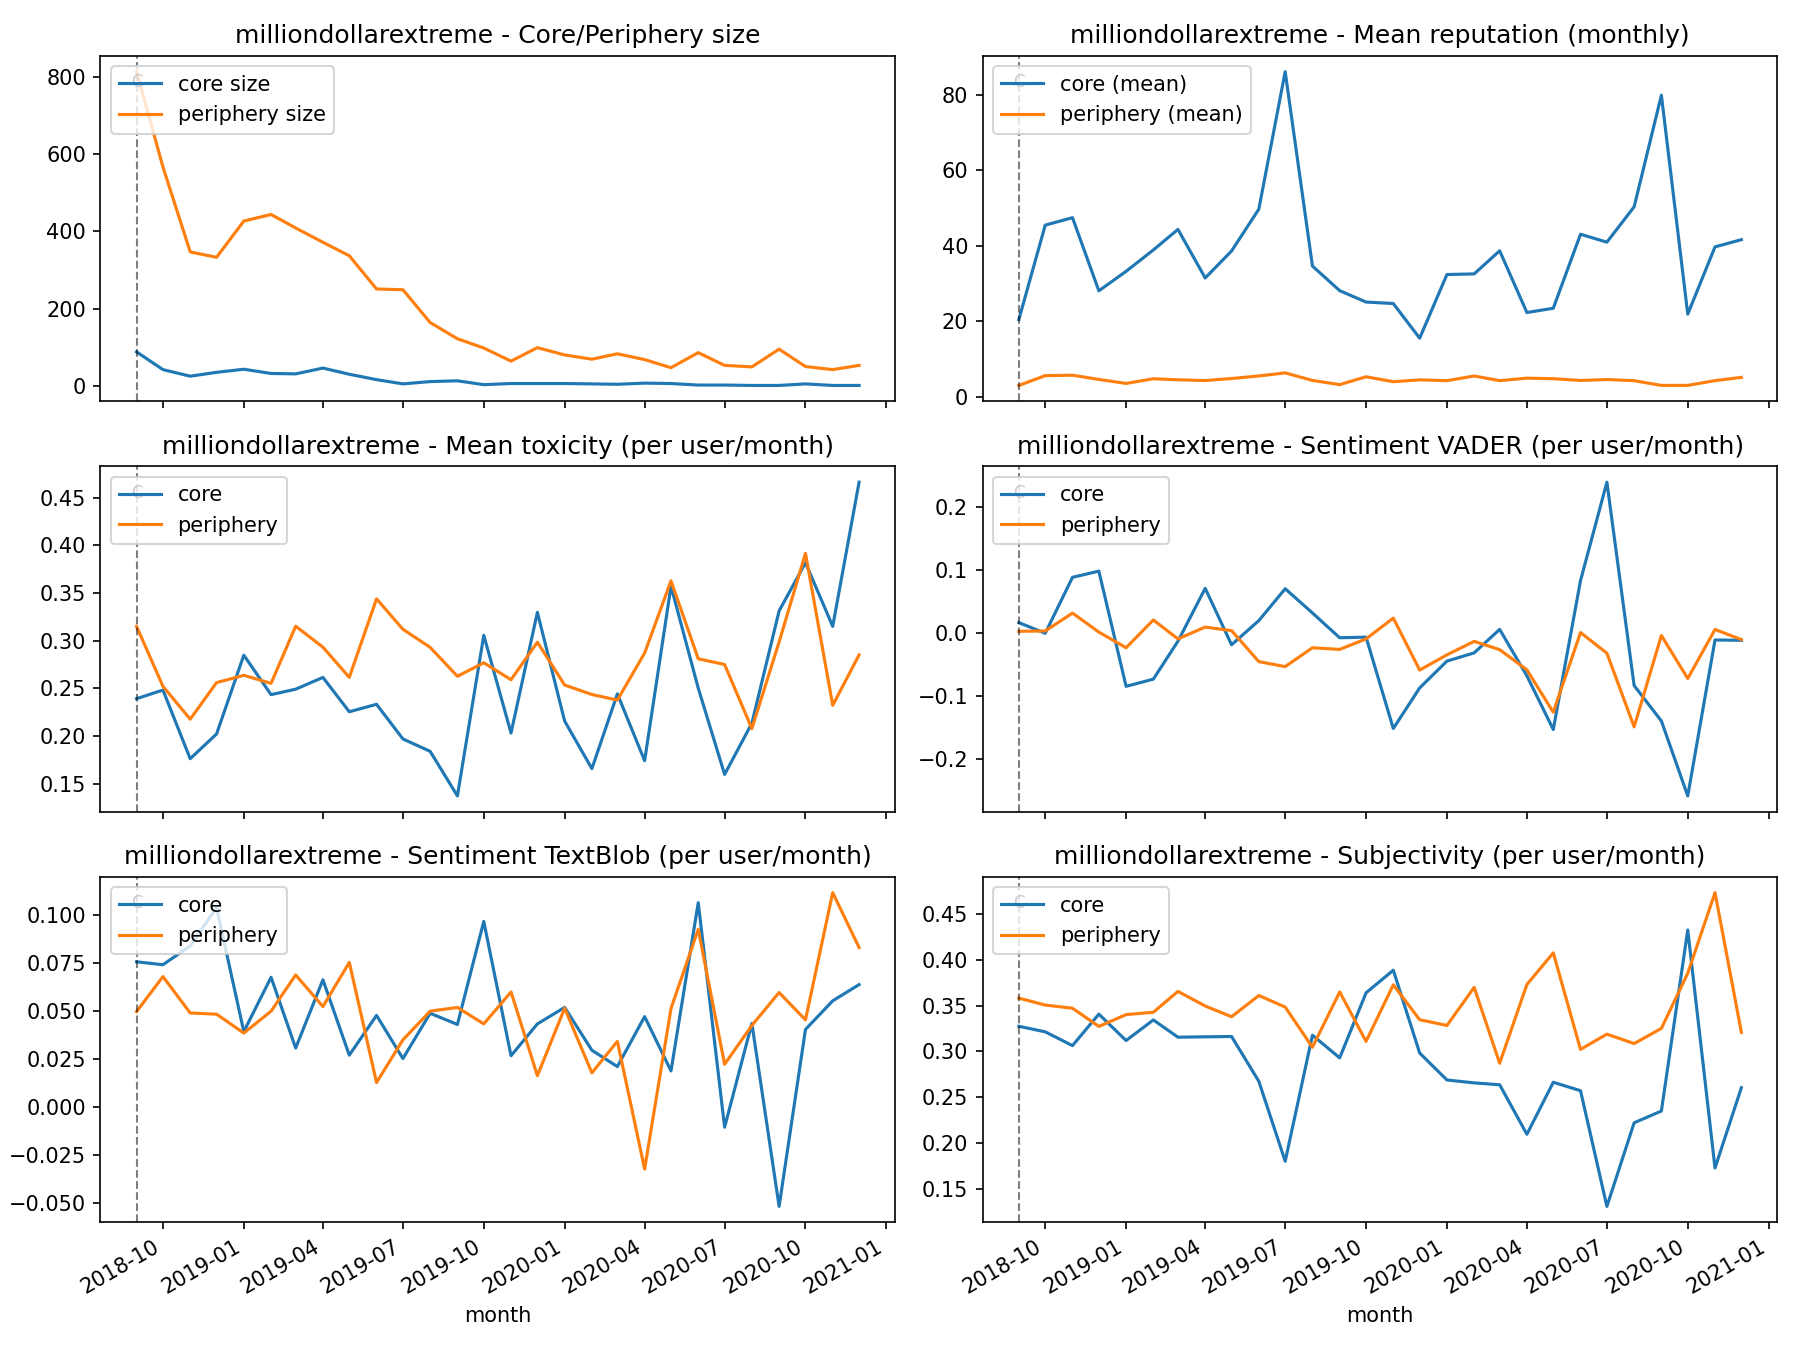
\includegraphics[width=\textwidth]{results/core-periphery/voat/figures/voat_milliondollarextreme_cp_panels_2col.png}
\end{frame}

\begin{frame}{Key Insights: MillionDollarExtreme - Voat}
\begin{itemize}
    \item \textbf{Post-2018 ban sustained activity}: Periphery starts at 650 after r/MillionDollarExtreme ban, gradually declines to 100—banned edgy comedy community maintained presence through platform shutdown
    \item \textbf{Consistently high toxicity}: Both core and periphery maintain 0.25-0.40 toxicity throughout timeline, converging at end—ironic/transgressive humor culture normalized extreme language
    \item \textbf{Core reputation volatility}: Core reputation oscillates 20-80 with dramatic spikes—small core ($\sim$50 users) showed unstable hierarchy, lacking established opinion leaders
\end{itemize}
\end{frame}

% -------------------------------------------------------------------
% Pics - Voat
% -------------------------------------------------------------------
\begin{frame}{Pics - Voat}
\centering
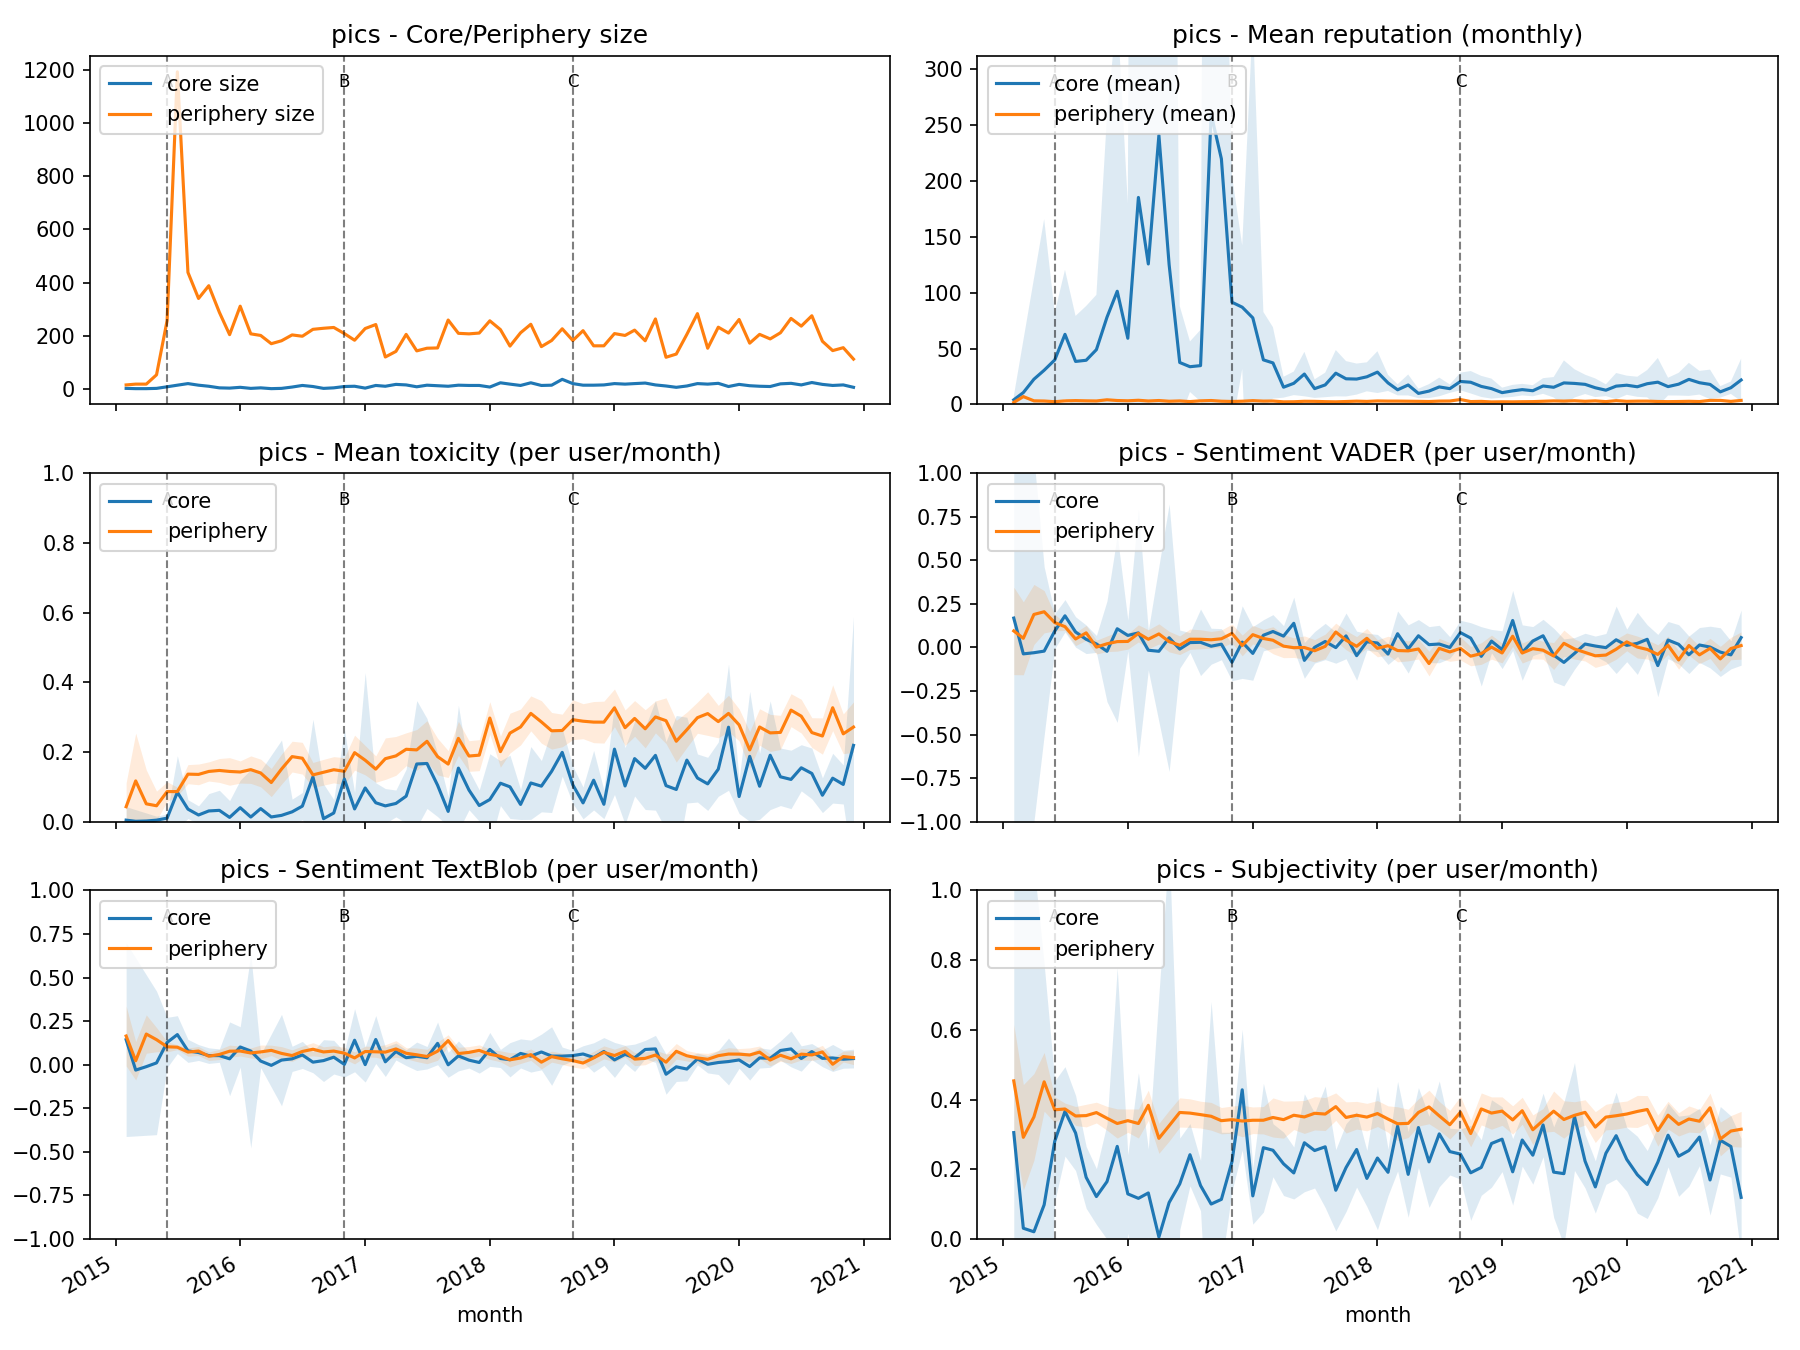
\includegraphics[width=\textwidth]{results/core-periphery/voat/figures/voat_pics_cp_panels_2col.png}
\end{frame}

\begin{frame}{Key Insights: Pics - Voat}
\begin{itemize}
    \item \textbf{Event A massive surge then stabilization}: Periphery spikes to 1000 (2015), stabilizes at 200-300—v/pics attracted substantial r/fatpeoplehate migrants seeking generalist content alongside v/funny
    \item \textbf{Escalating periphery toxicity}: Periphery toxicity climbs from 0.10 to 0.30 (2015-2021), while core rises from 0.05 to 0.20—both radicalized but periphery consistently worse
    \item \textbf{Core reputation spikes then collapse}: Core reputation surges to 180-220 around 2016-2017, crashes to $<$20 by 2019—early high-status migrants abandoned community as culture deteriorated
\end{itemize}
\end{frame}

% -------------------------------------------------------------------
% Technology - Voat
% -------------------------------------------------------------------
\begin{frame}{Technology - Voat}
\centering
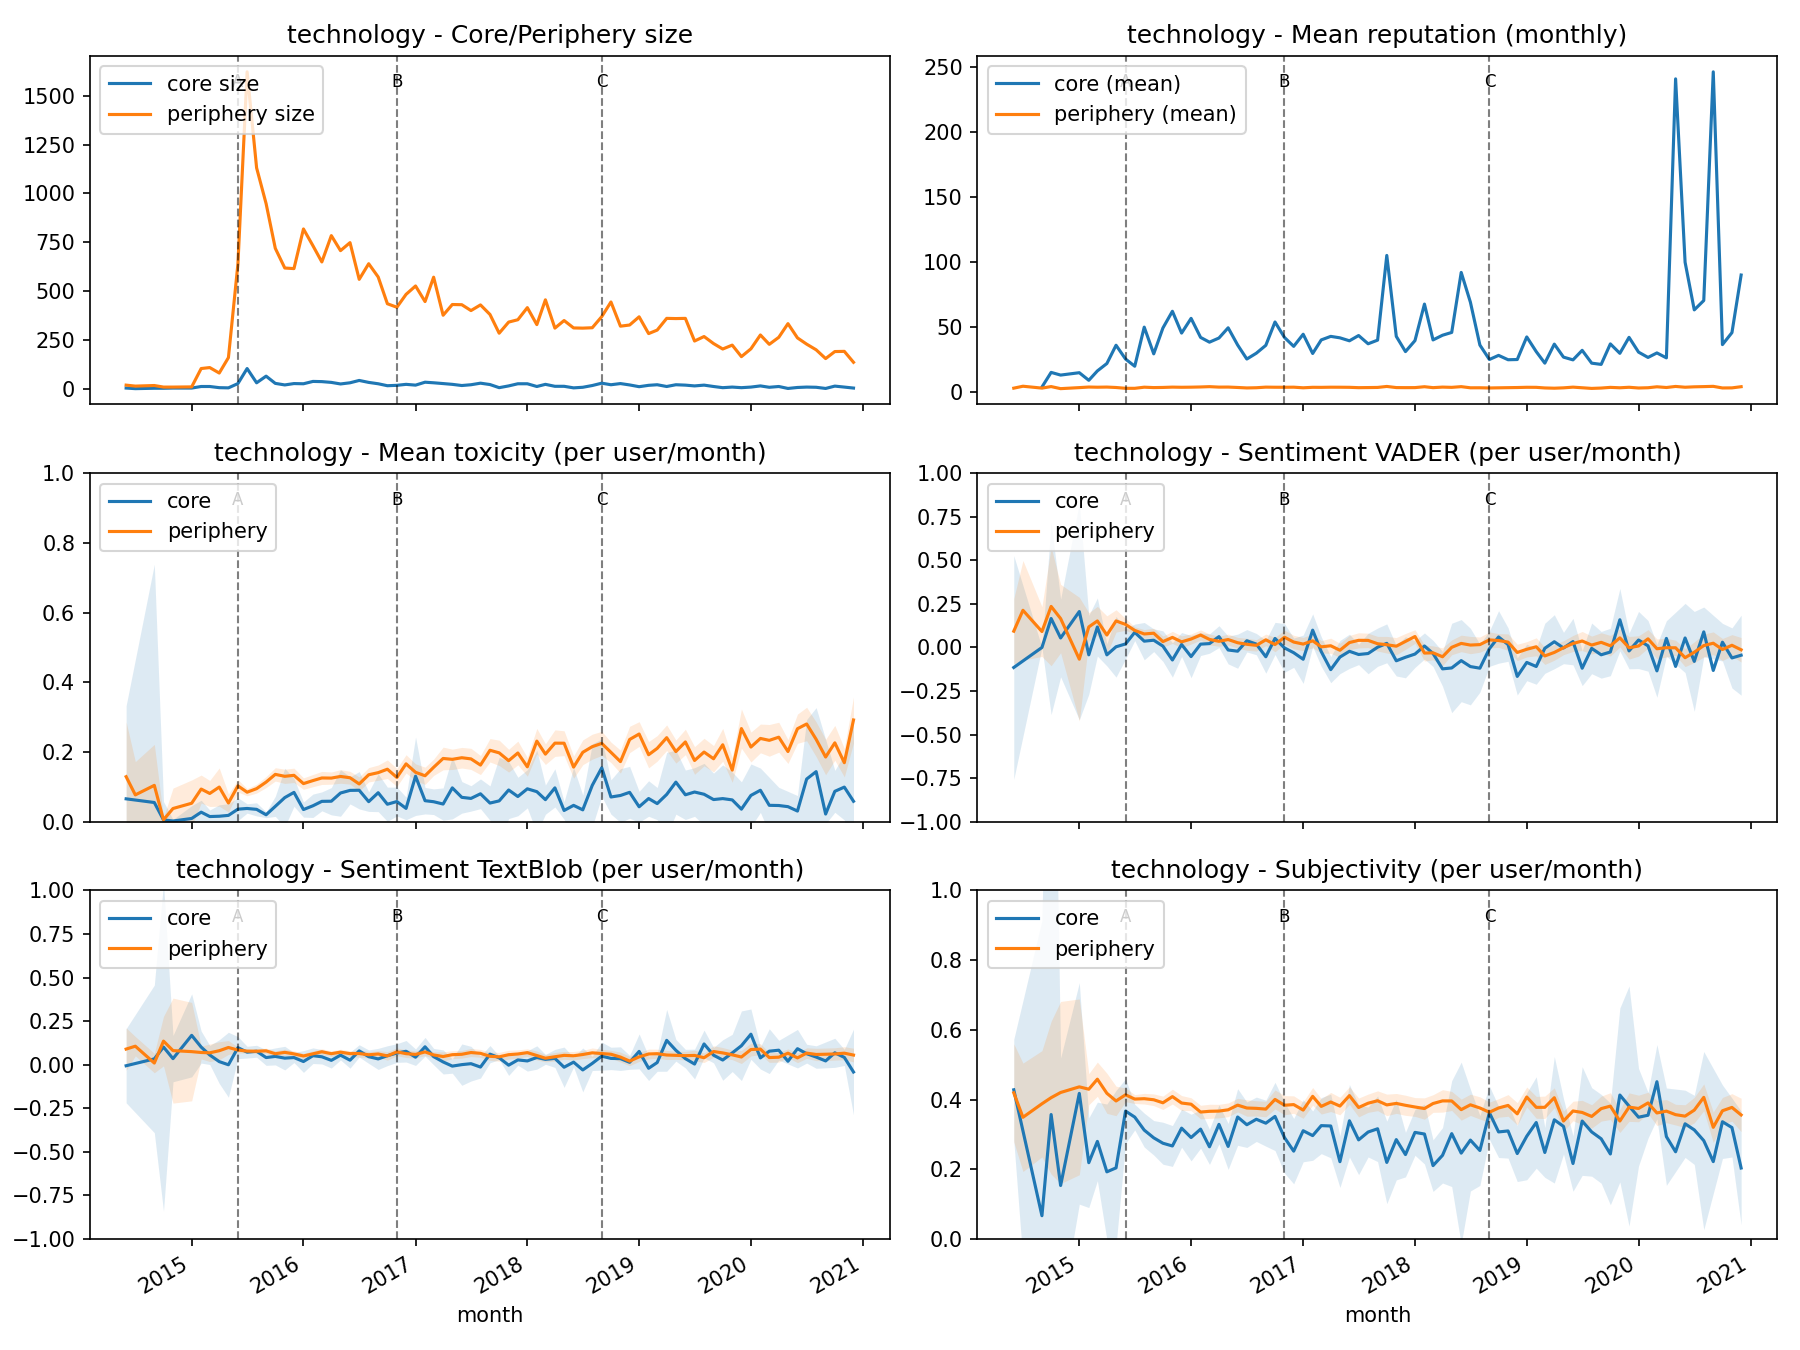
\includegraphics[width=\textwidth]{results/core-periphery/voat/figures/voat_technology_cp_panels_2col.png}
\end{frame}

\begin{frame}{Key Insights: Technology - Voat}
\begin{itemize}
    \item \textbf{Event A surge with sustained base}: Periphery peaks at 1300 (2015), stabilizes at 300-400—v/technology retained significant generalist migrants interested in privacy/censorship discussions aligned with Voat's ethos
    \item \textbf{Escalating periphery toxicity}: Periphery toxicity climbs from 0.10 to 0.25 (2015-2021) while core stays lower (0.05-0.10)—tech discussions increasingly politicized
    \item \textbf{Late core reputation surge}: Core reputation jumps to 250 in 2020-2021 (near shutdown), mirroring Reddit pattern—possible artifact or final concentration of veteran users
\end{itemize}
\end{frame}

% -------------------------------------------------------------------
% Videos - Voat
% -------------------------------------------------------------------
\begin{frame}{Videos - Voat}
\centering
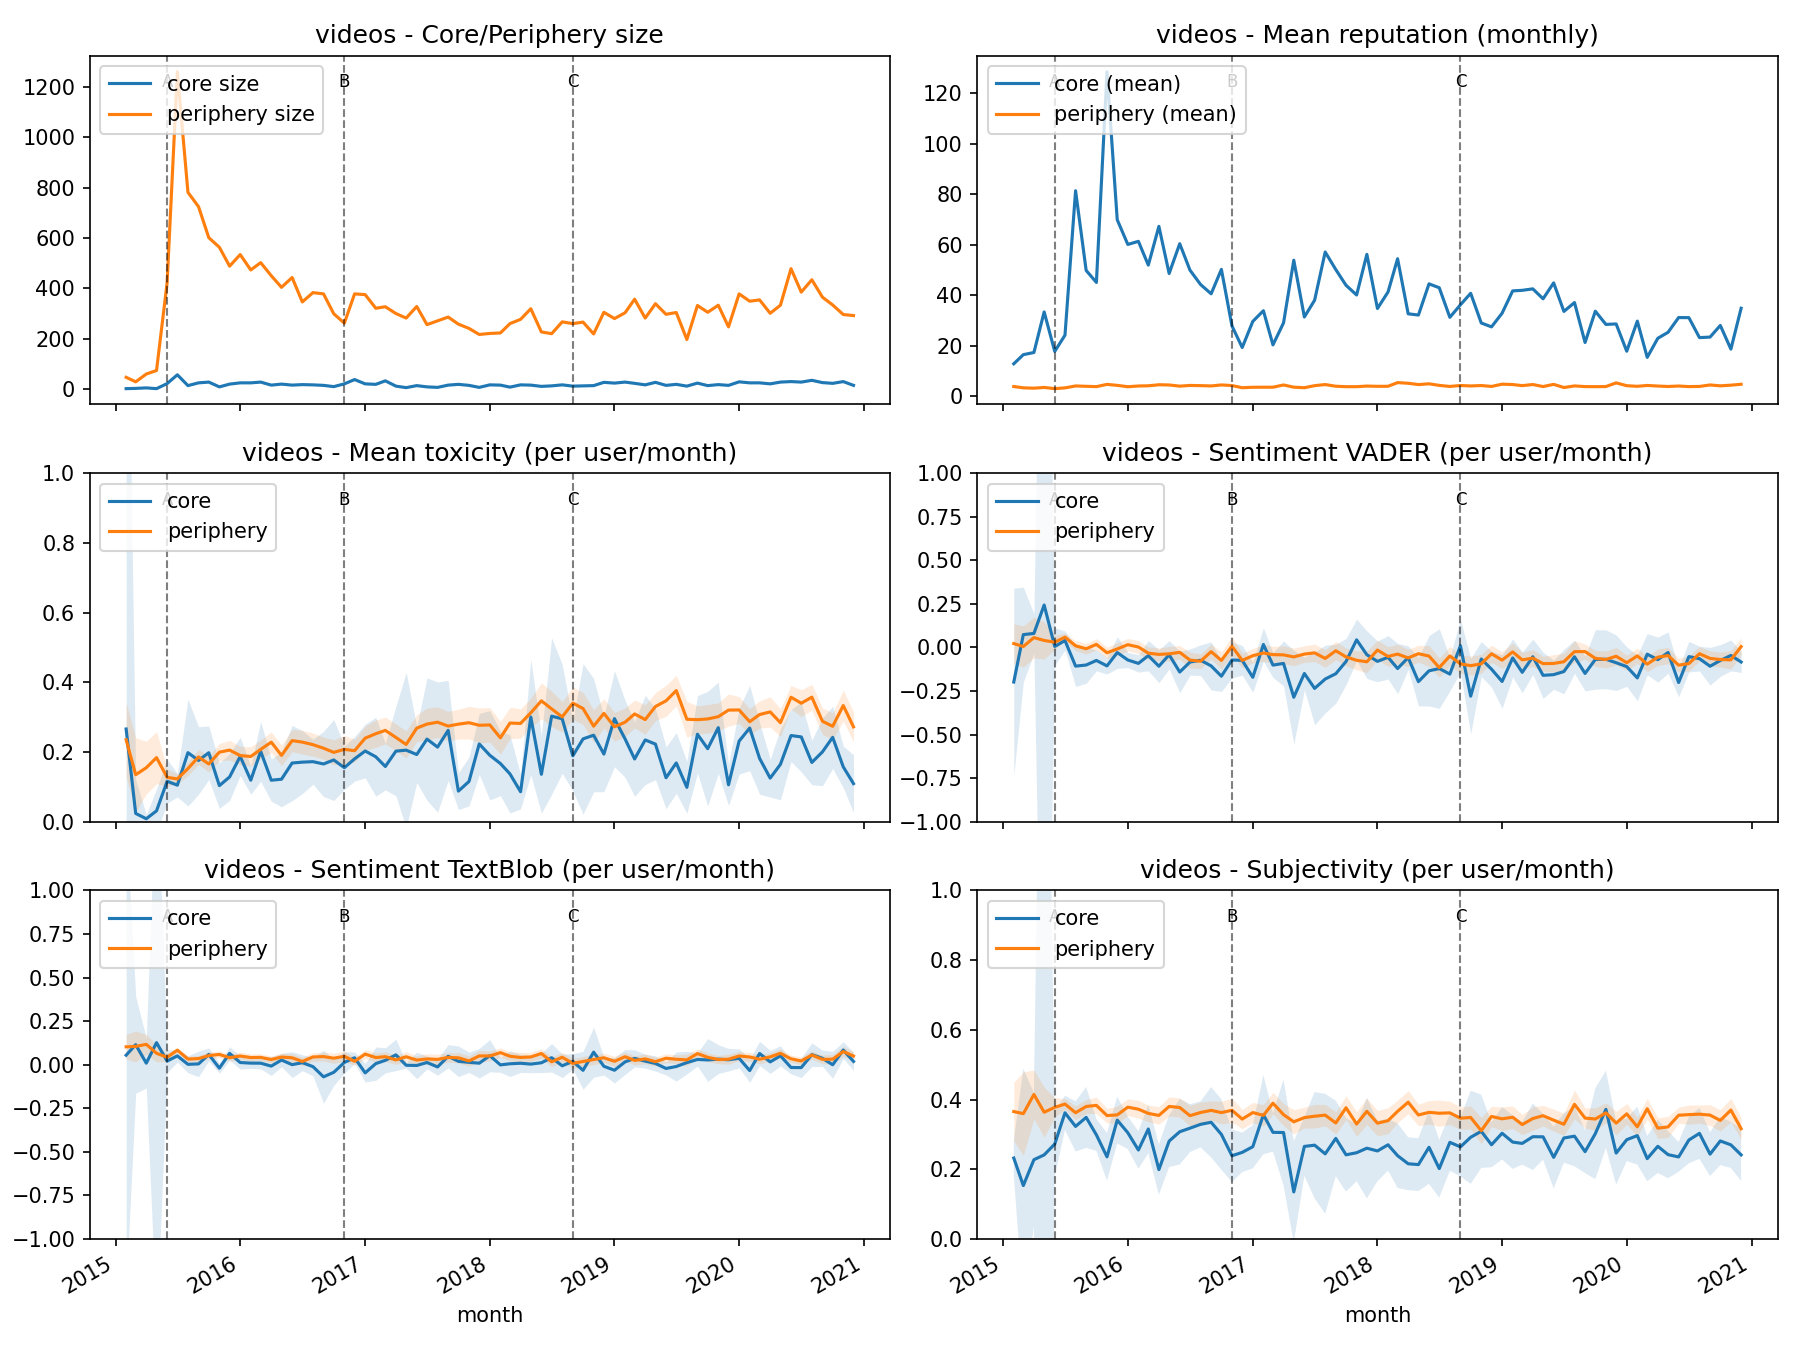
\includegraphics[width=\textwidth]{results/core-periphery/voat/figures/voat_videos_cp_panels_2col.png}
\end{frame}

\begin{frame}{Key Insights: Videos - Voat}
\begin{itemize}
    \item \textbf{Event A surge with moderate retention}: Periphery peaks at 1000 (2015), stabilizes at 300-400—v/videos retained generalist migrants similarly to v/funny and v/pics as major entertainment hub
    \item \textbf{Converging high toxicity}: Core and periphery converge at 0.25-0.35 toxicity by 2019-2021—video discussions became uniformly radicalized as platform culture homogenized
    \item \textbf{Core reputation decline}: Core reputation drops from 100 to 20 (2015-2021)—early high-status users left, remaining core lost influence as community fragmented
\end{itemize}
\end{frame}

% SECTION: Core Time Series Analysis
% ===================================================================
\section{Core Time Series Analysis}

% -------------------------------------------------------------------
% Funny Community
% -------------------------------------------------------------------
\begin{frame}{Funny Community}
\centering
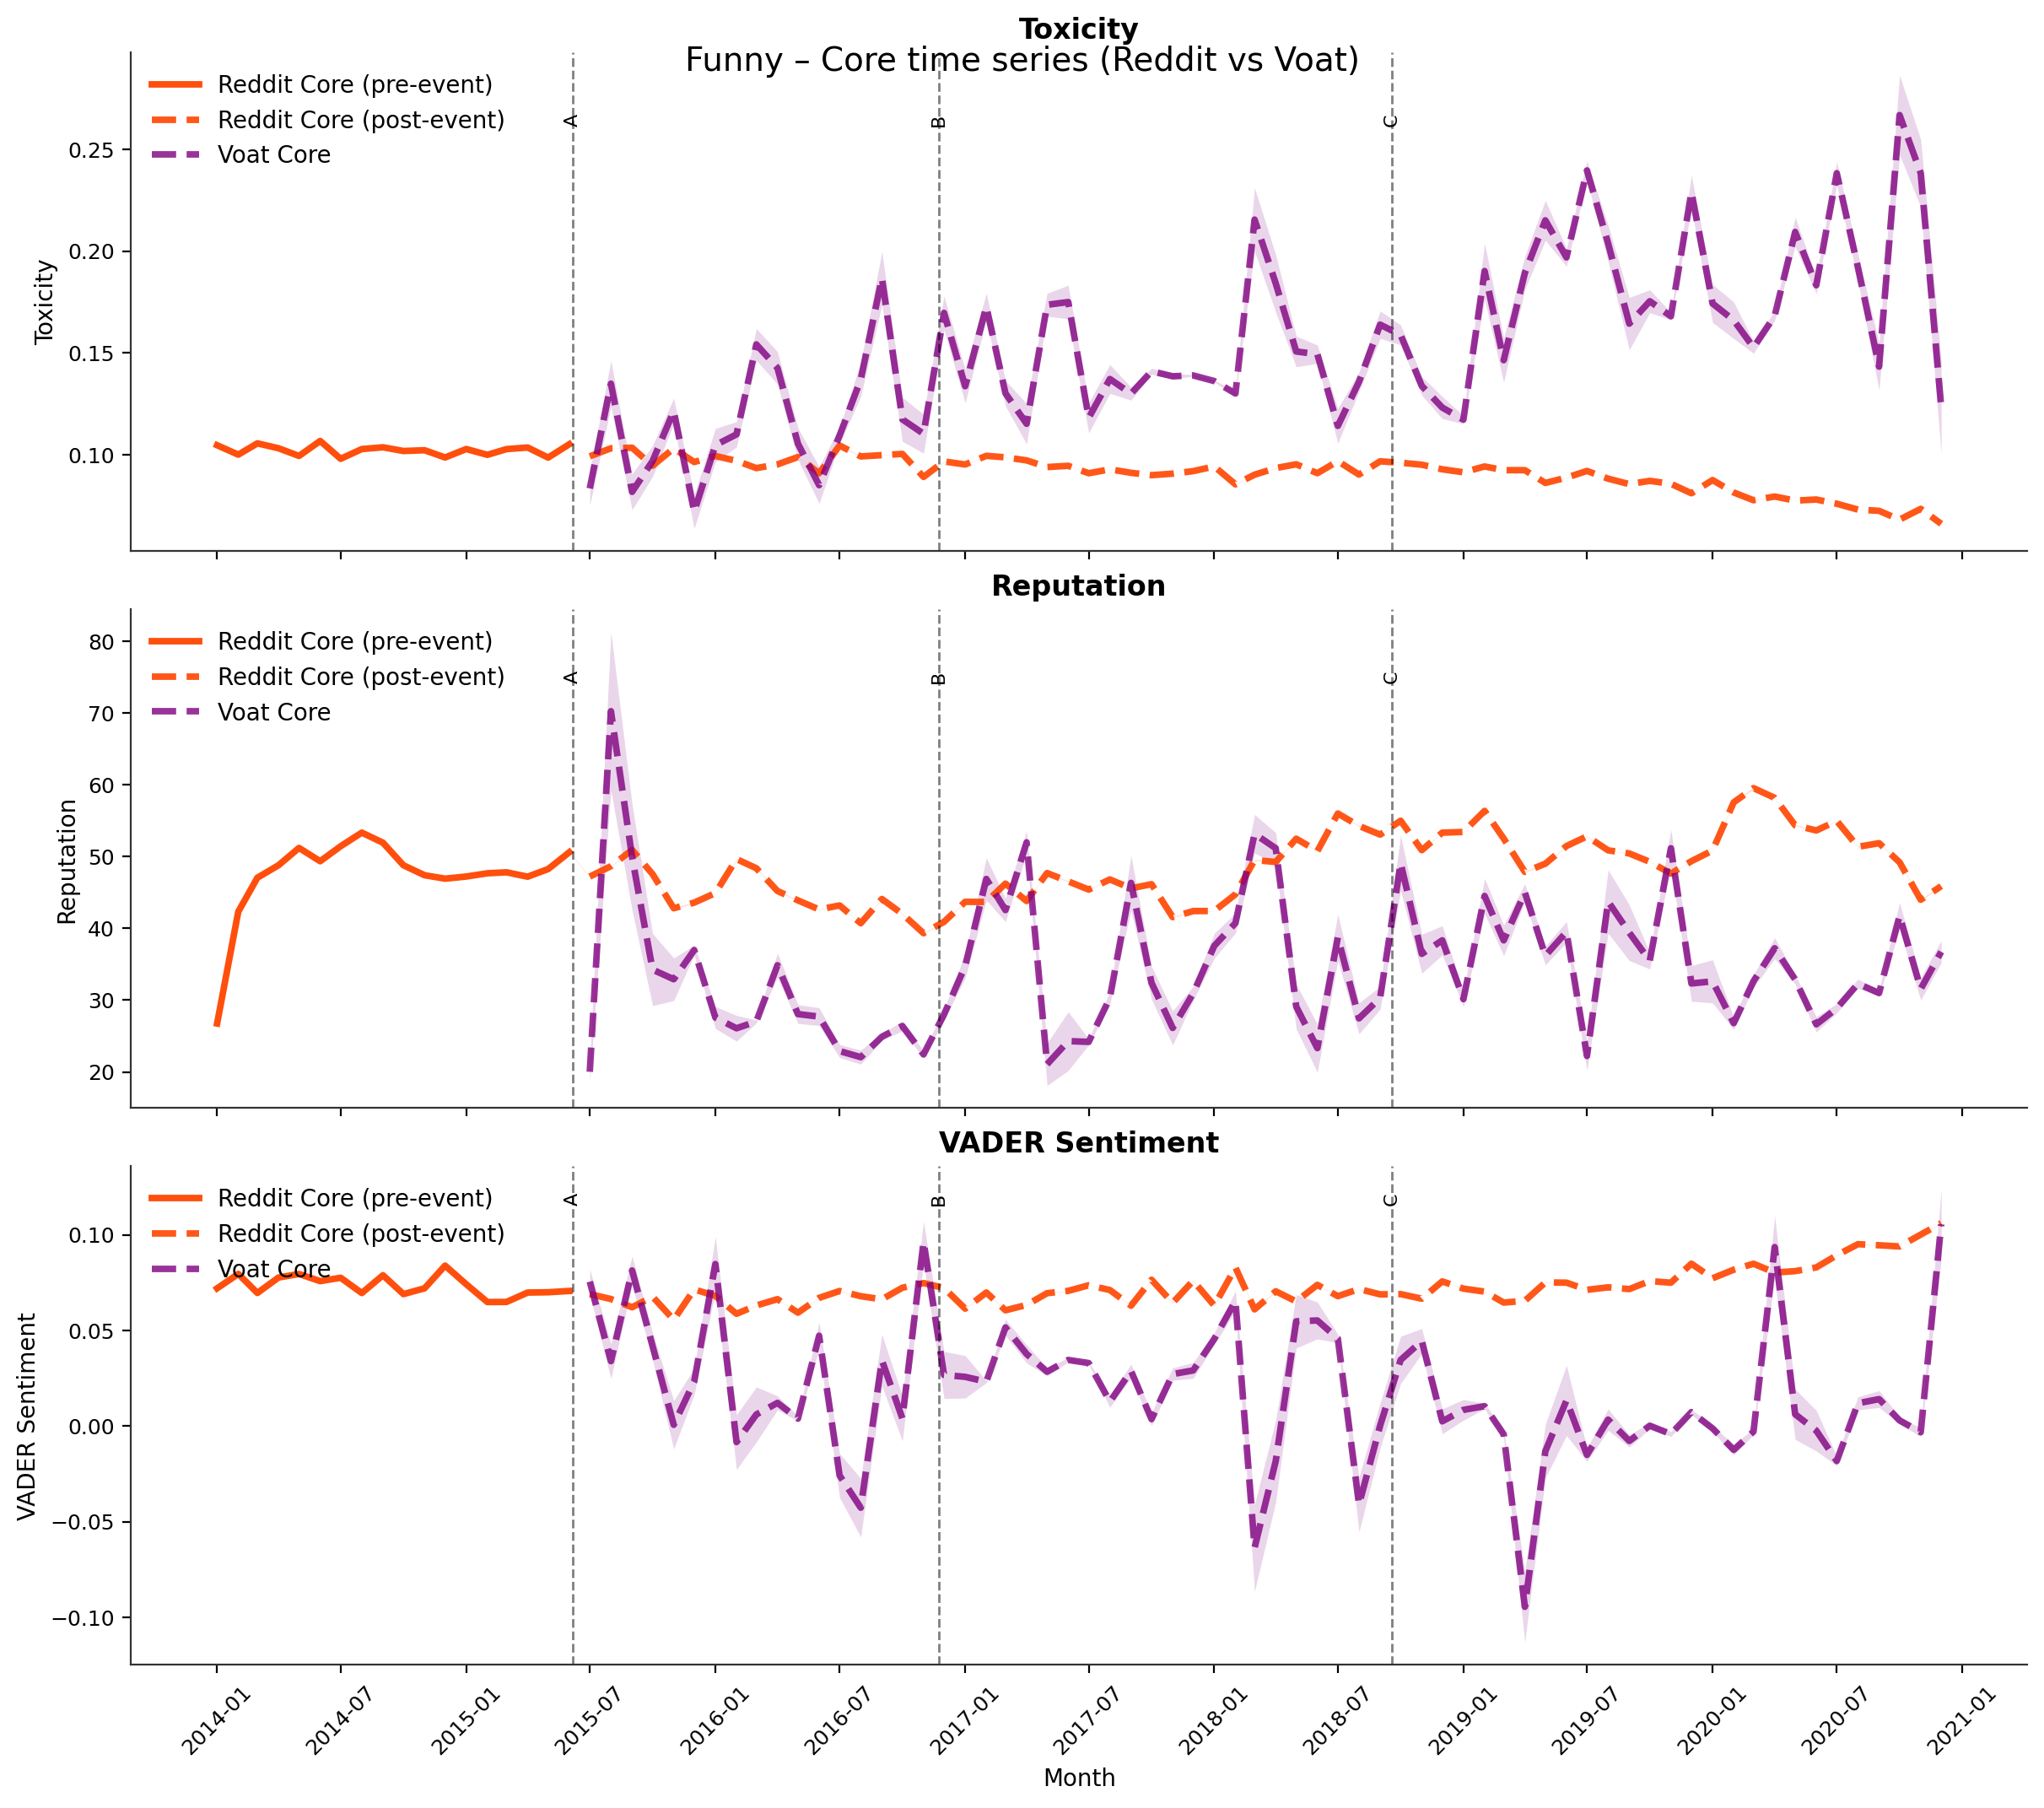
\includegraphics[width=\textwidth]{results/basic/funny/compare/figures/funny_timeseries_panels.png}
\end{frame}

\begin{frame}{Key Insights: Funny Community}
\begin{itemize}
    \item \textbf{Platform divergence post-ban}: Event A (2015 harassment policy) marks sharp separation—Voat Core toxicity doubles to 0.15-0.25 while Reddit Core remains stable at $\sim$0.10
    \item \textbf{Migration wave effects}: Reputation spike at Event A reflects influx of generalist migrants (e.g., r/fatpeoplehate users), followed by decline as later conspiracy-focused waves (Events B, C) brought more volatile, lower-reputation users
    \item \textbf{Sentiment polarization}: Reddit Core sustains positive affect (0.05-0.10); Voat Core oscillates near neutral/negative, reflecting concentration of displaced users with antisocial norms
\end{itemize}
\end{frame}

% -------------------------------------------------------------------
% Gaming Community
% -------------------------------------------------------------------
\begin{frame}{Gaming Community}
\centering
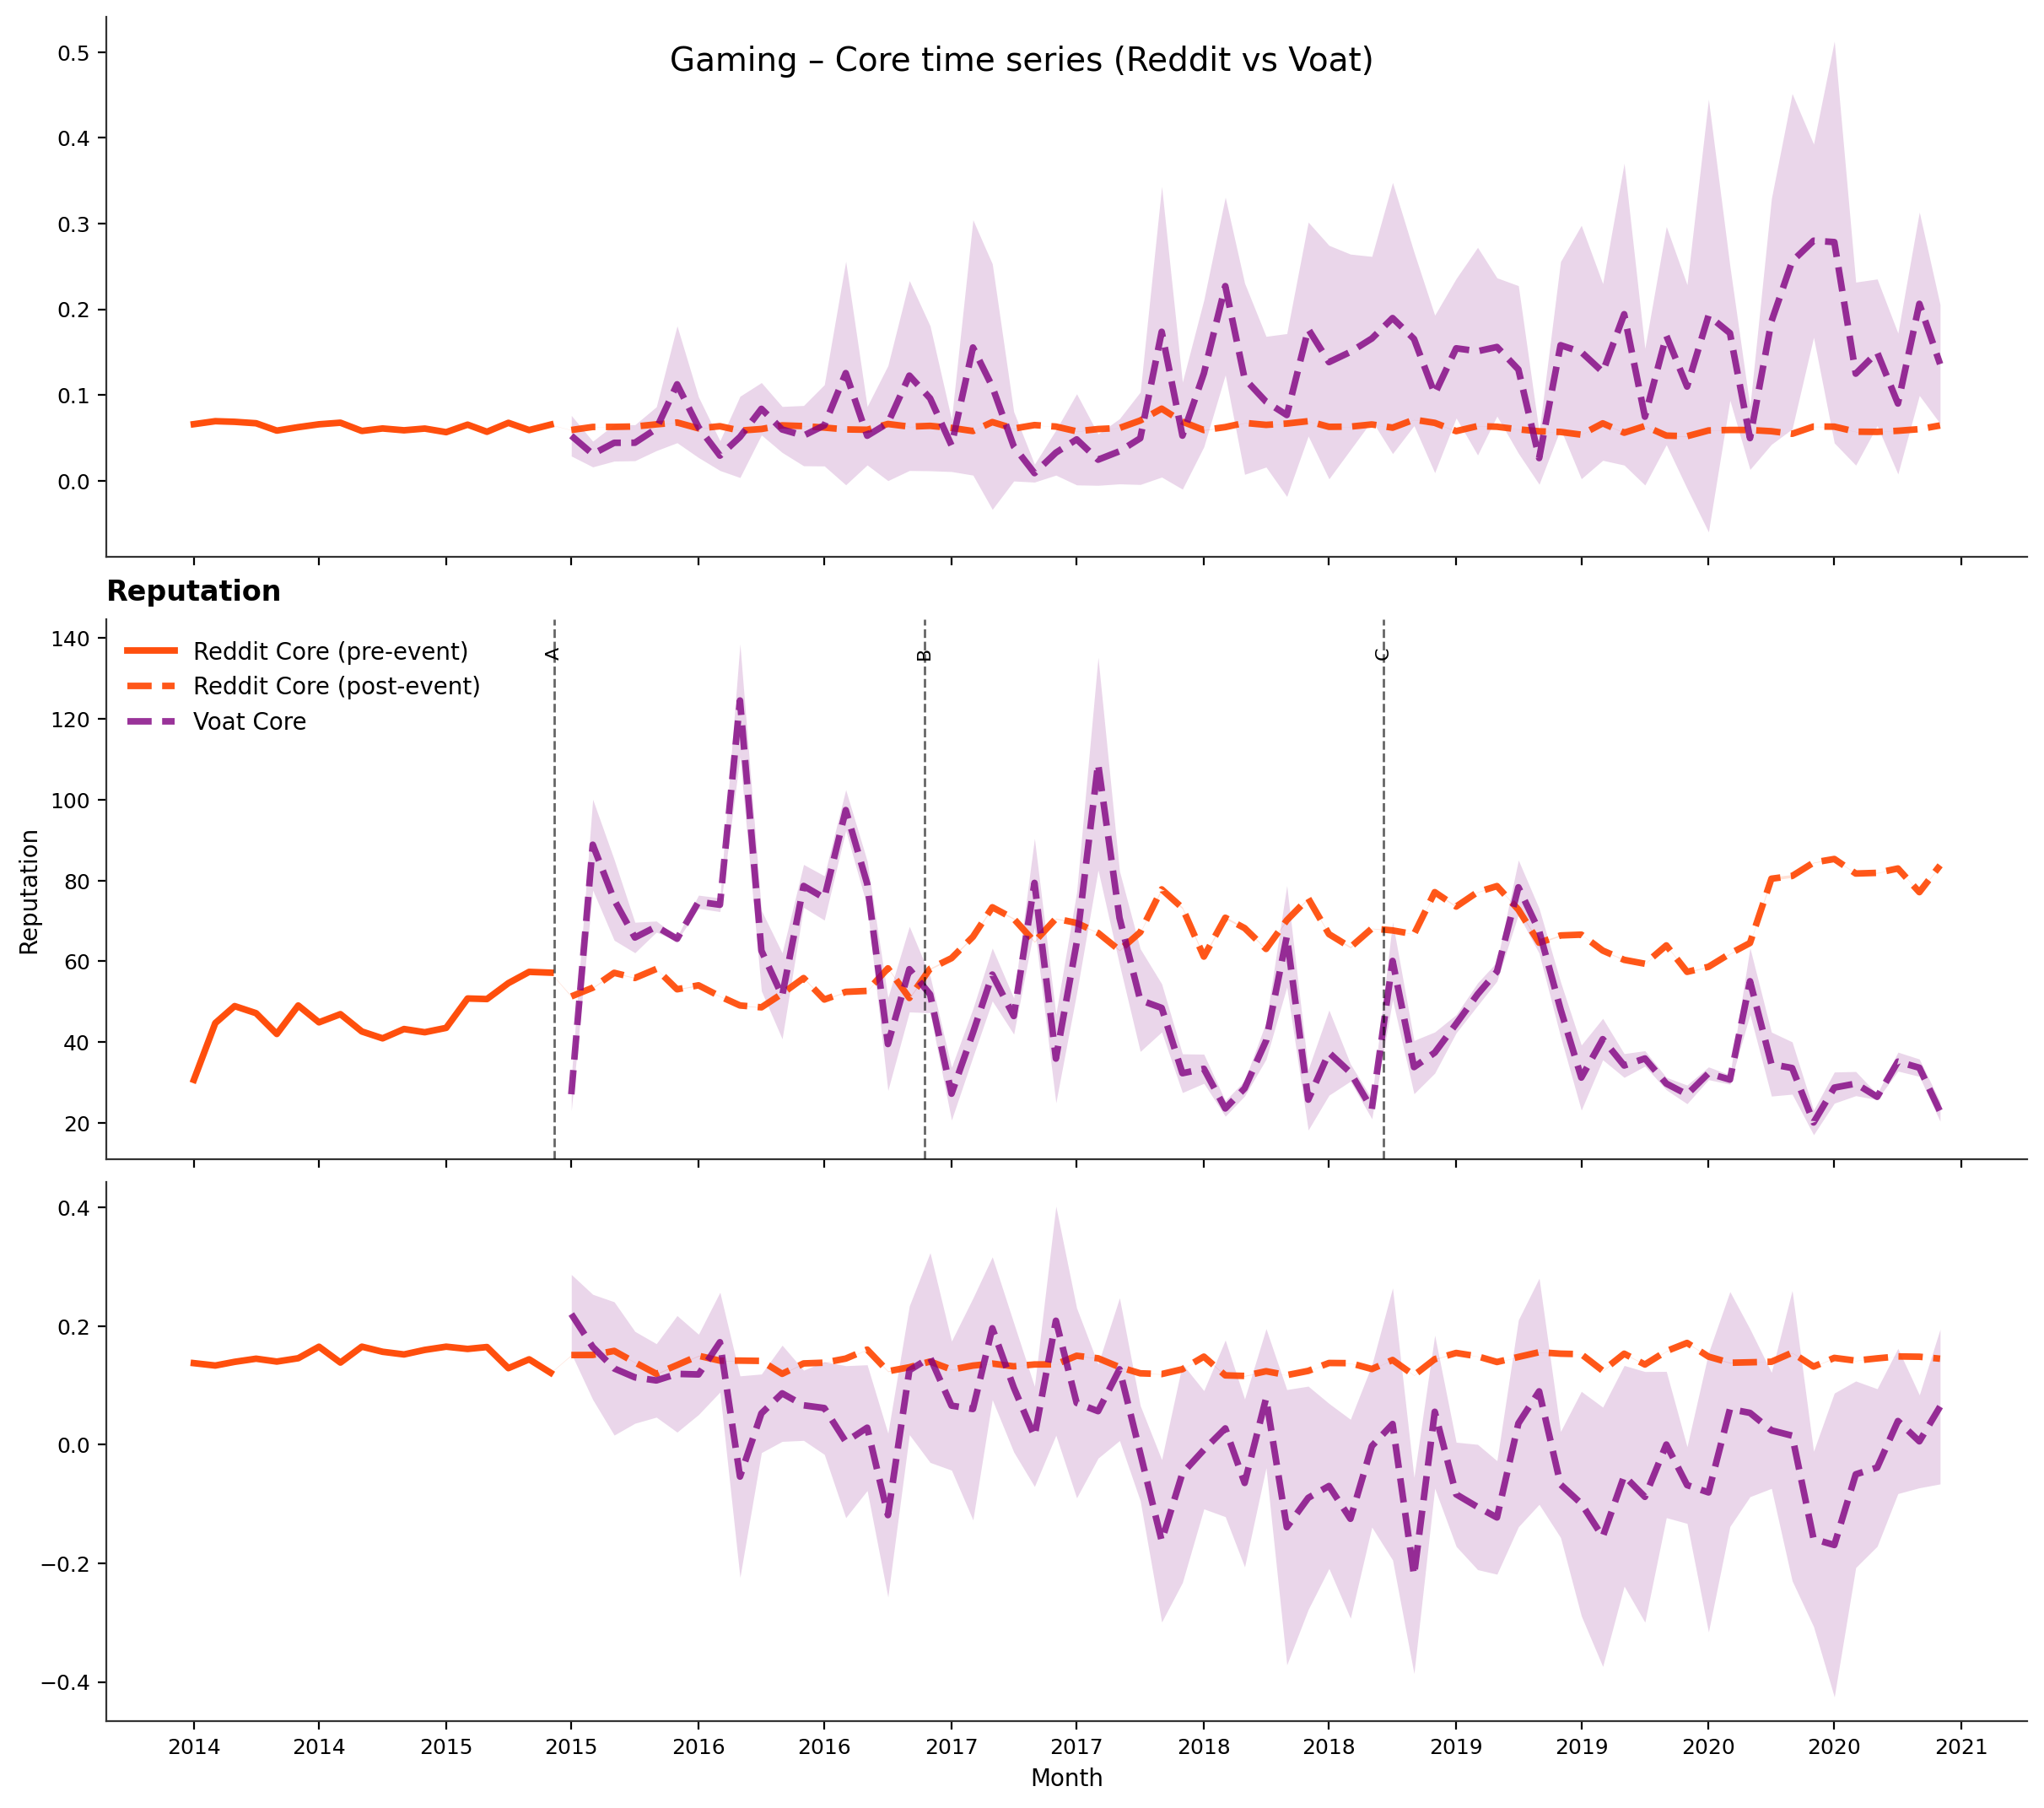
\includegraphics[width=\textwidth]{results/basic/gaming/compare/figures/gaming_timeseries_panels.png}
\end{frame}

\begin{frame}{Key Insights: Gaming Community}
\begin{itemize}
    \item \textbf{Catastrophic reputation collapse}: Voat Core reputation spikes to 120+ at Event A (r/fatpeoplehate migrants joining generalist subverses), then crashes to 20-30 by Event C as conspiracy-focused waves starved /v/gaming of new connectors
    \item \textbf{Extreme toxicity volatility}: Voat Core toxicity fluctuates wildly (0.0-0.5 range with massive variance), contrasting with Reddit's flat $\sim$0.05-0.07 stability—reflecting high turnover and loss of cohesive core
    \item \textbf{Sentiment erosion}: Voat Core sentiment trends increasingly negative post-Event B, hovering near -0.2 by 2020, while Reddit Core maintains stable positive affect ($\sim$0.12-0.15)
\end{itemize}
\end{frame}

% -------------------------------------------------------------------
% Gifs Community
% -------------------------------------------------------------------
\begin{frame}{Gifs Community}
\centering
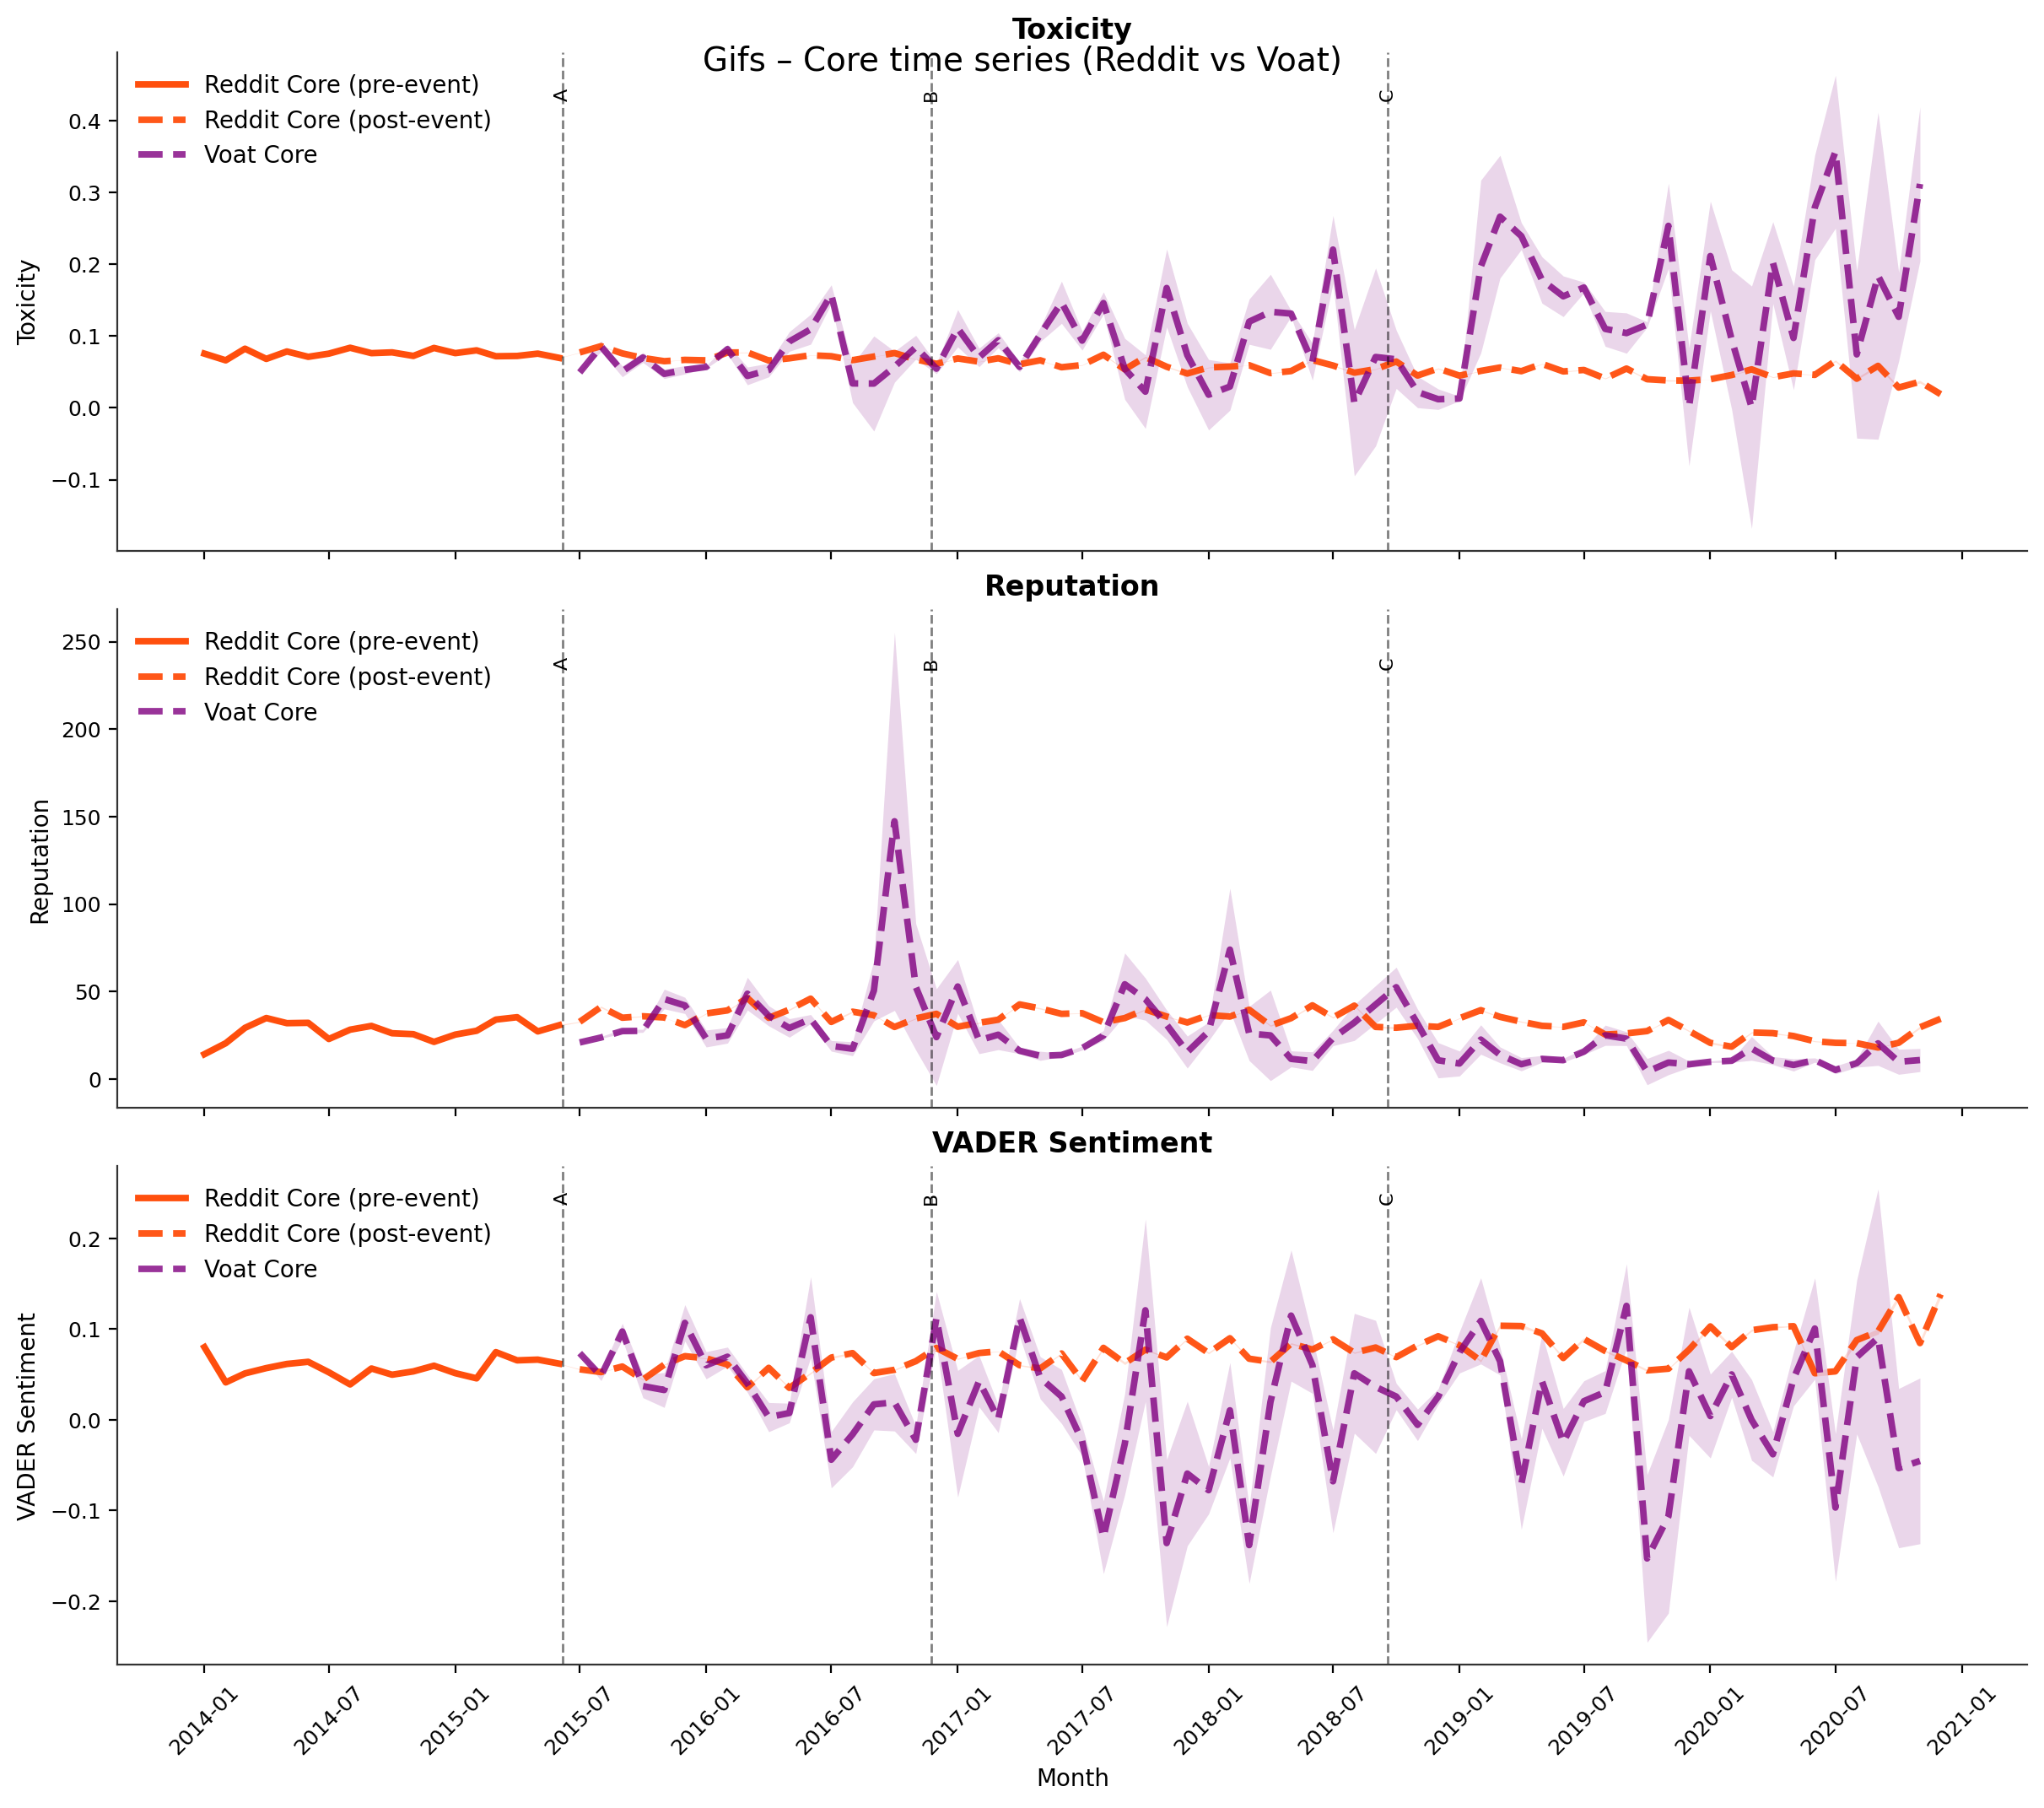
\includegraphics[width=\textwidth]{results/basic/gifs/compare/figures/gifs_timeseries_panels.png}
\end{frame}

\begin{frame}{Key Insights: Gifs Community}
\begin{itemize}
    \item \textbf{Delayed toxicity escalation}: Voat Core toxicity remains modest (0.05-0.15) until Event C (2018 QAnon ban), then surges to 0.25-0.40 by 2019—suggesting late-arriving conspiracy users colonized this generalist space
    \item \textbf{Converging low reputation}: Both platforms show declining reputation trends, converging around 20-30 by 2020, indicating /v/gifs failed to retain high-reputation generalist migrants from Event A
    \item \textbf{Persistent negative sentiment}: Voat Core sentiment drops sharply below zero after Event B and remains consistently negative (-0.05 to -0.15), while Reddit Core maintains positive affect (0.07-0.12)
\end{itemize}
\end{frame}

% -------------------------------------------------------------------
% Pics Community
% -------------------------------------------------------------------
\begin{frame}{Pics Community}
\centering
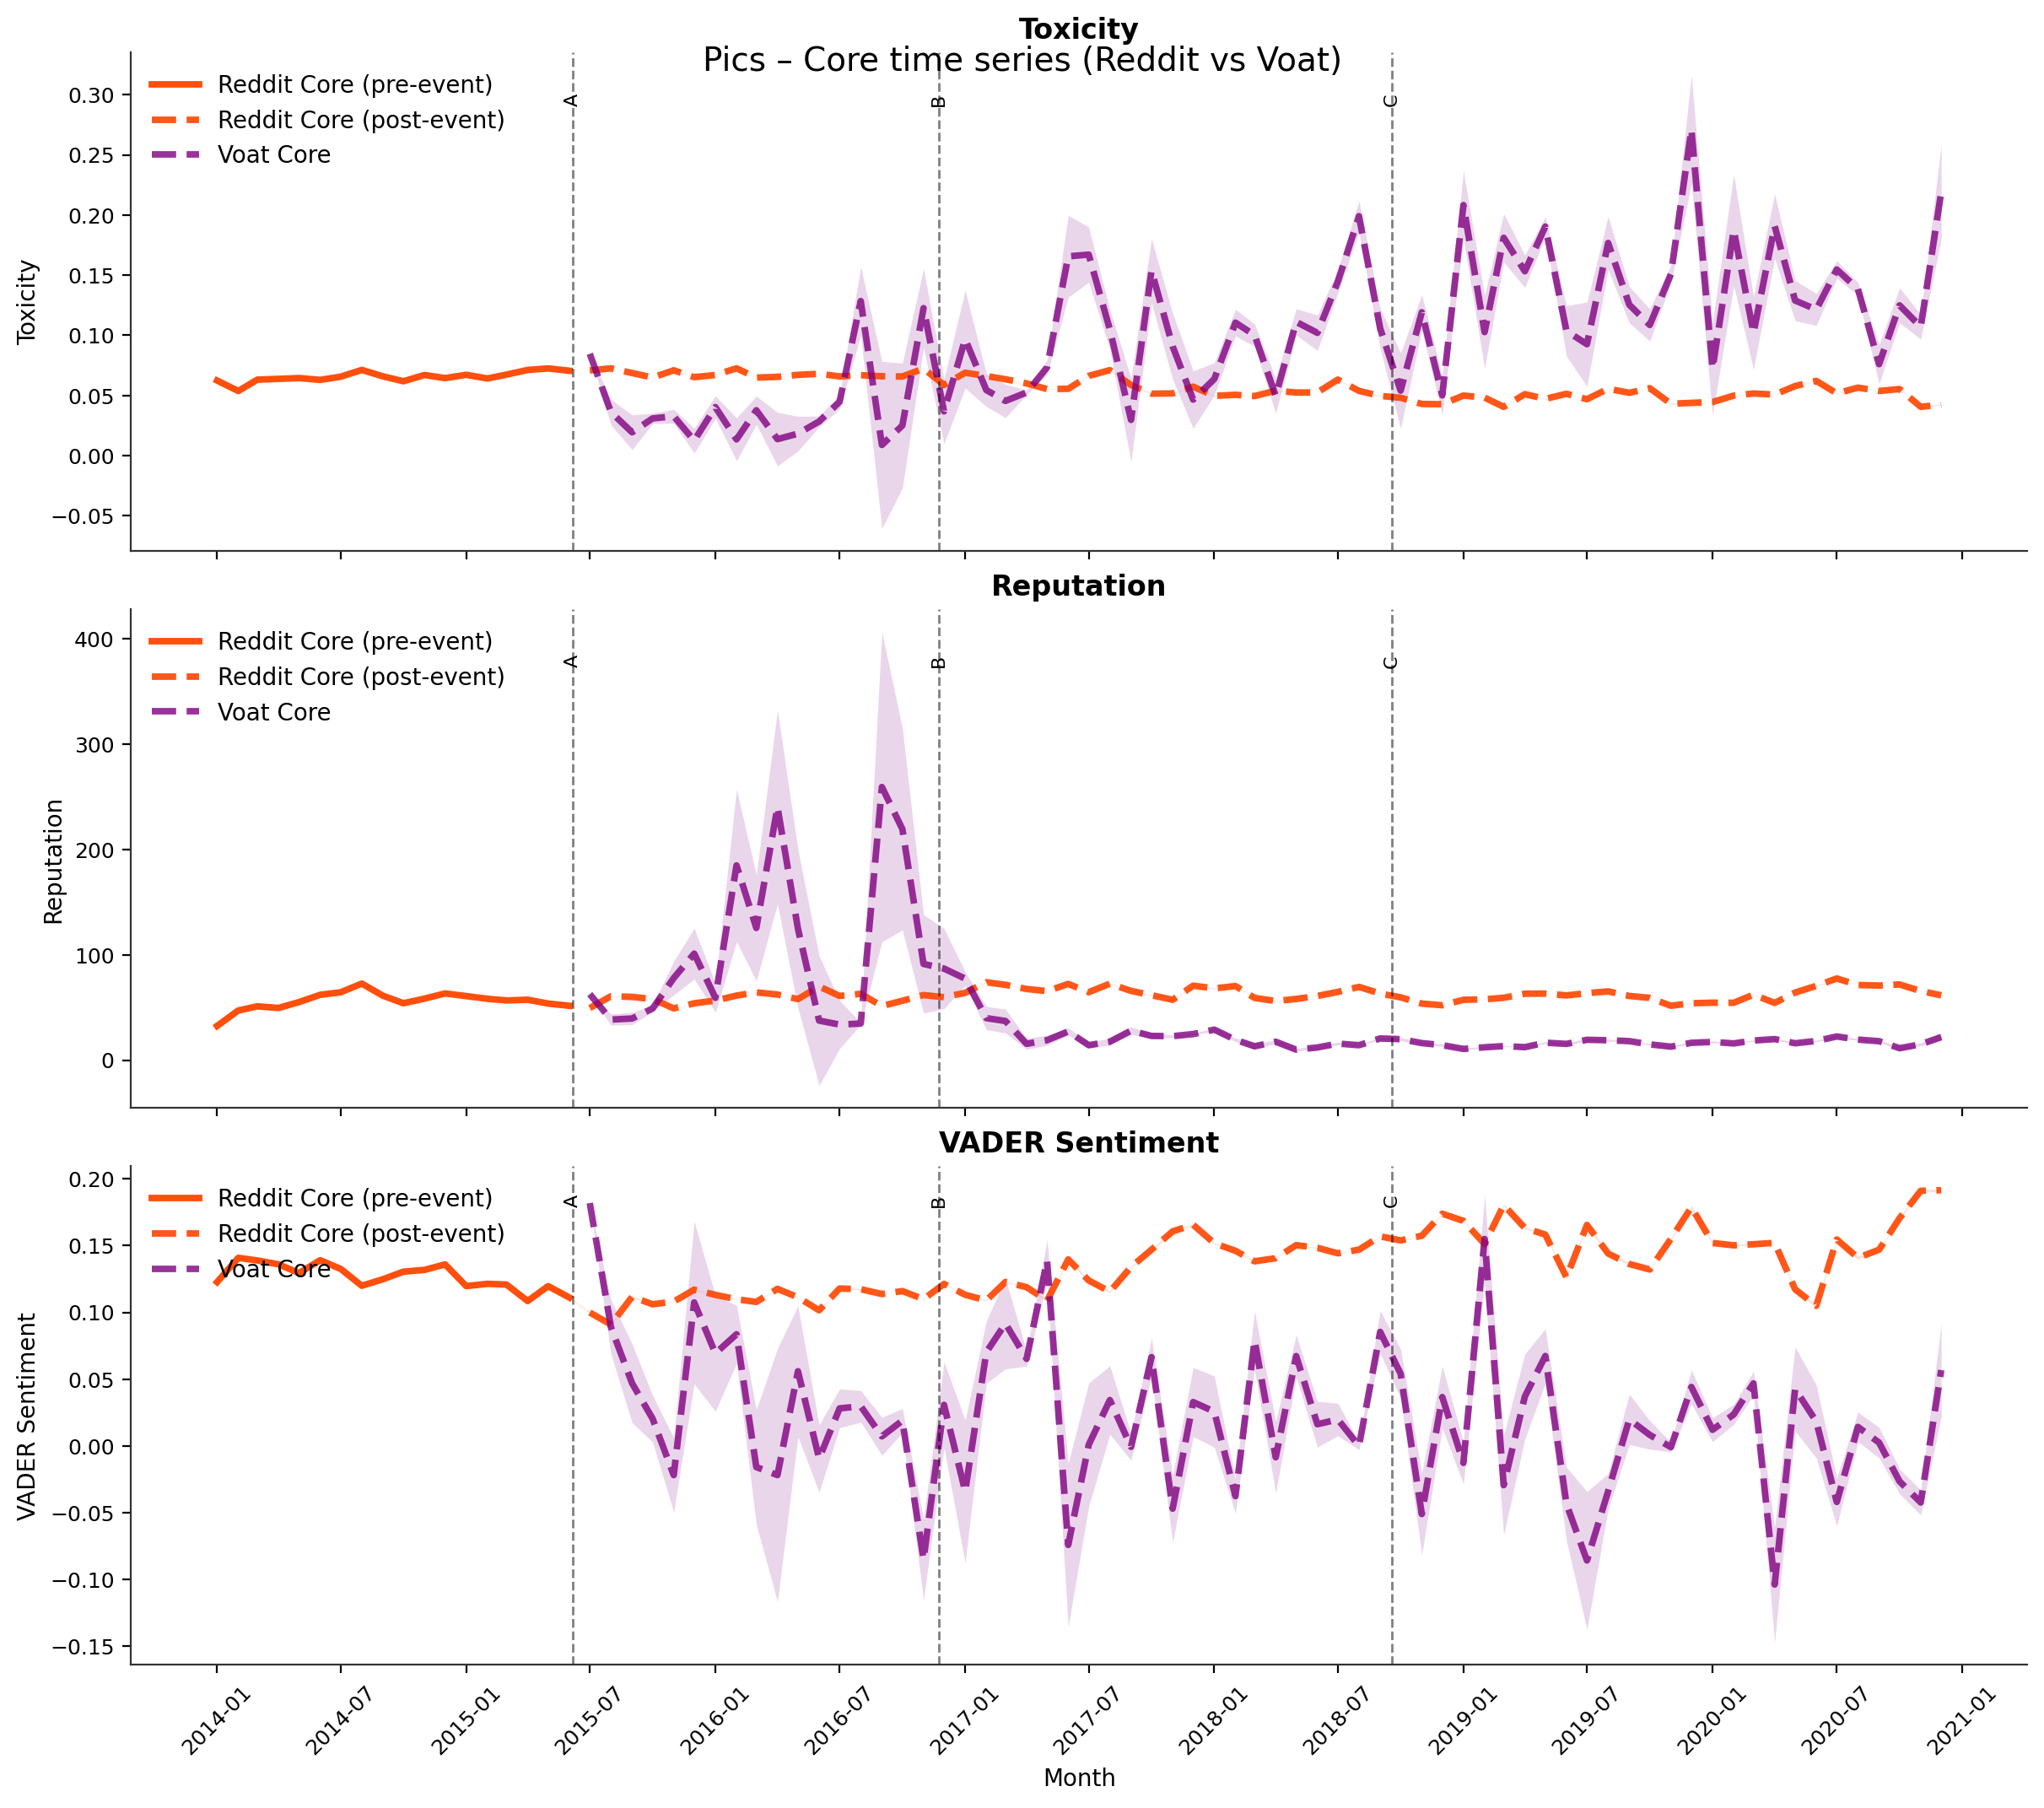
\includegraphics[width=\textwidth]{results/basic/pics/compare/figures/pics_timeseries_panels.png}
\end{frame}

\begin{frame}{Key Insights: Pics Community}
\begin{itemize}
    \item \textbf{Massive reputation spike then total collapse}: Voat Core reputation explodes to 250+ around Event A/B (highest among all generalist communities), then crashes to $<$25 and flatlines—indicating initial high-status migrants abandoned the community
    \item \textbf{Gradual toxicity creep}: Voat Core toxicity starts low ($\sim$0.02) but steadily escalates to 0.15-0.25 by 2019, tripling Reddit's stable $\sim$0.05 baseline as the community composition shifted
    \item \textbf{Sentiment floor effect}: Voat Core sentiment oscillates around zero with frequent dips to -0.10, never sustaining the positive affect (0.10-0.20) Reddit Core maintains throughout
\end{itemize}
\end{frame}

% -------------------------------------------------------------------
% Technology Community
% -------------------------------------------------------------------
\begin{frame}{Technology Community}
\centering
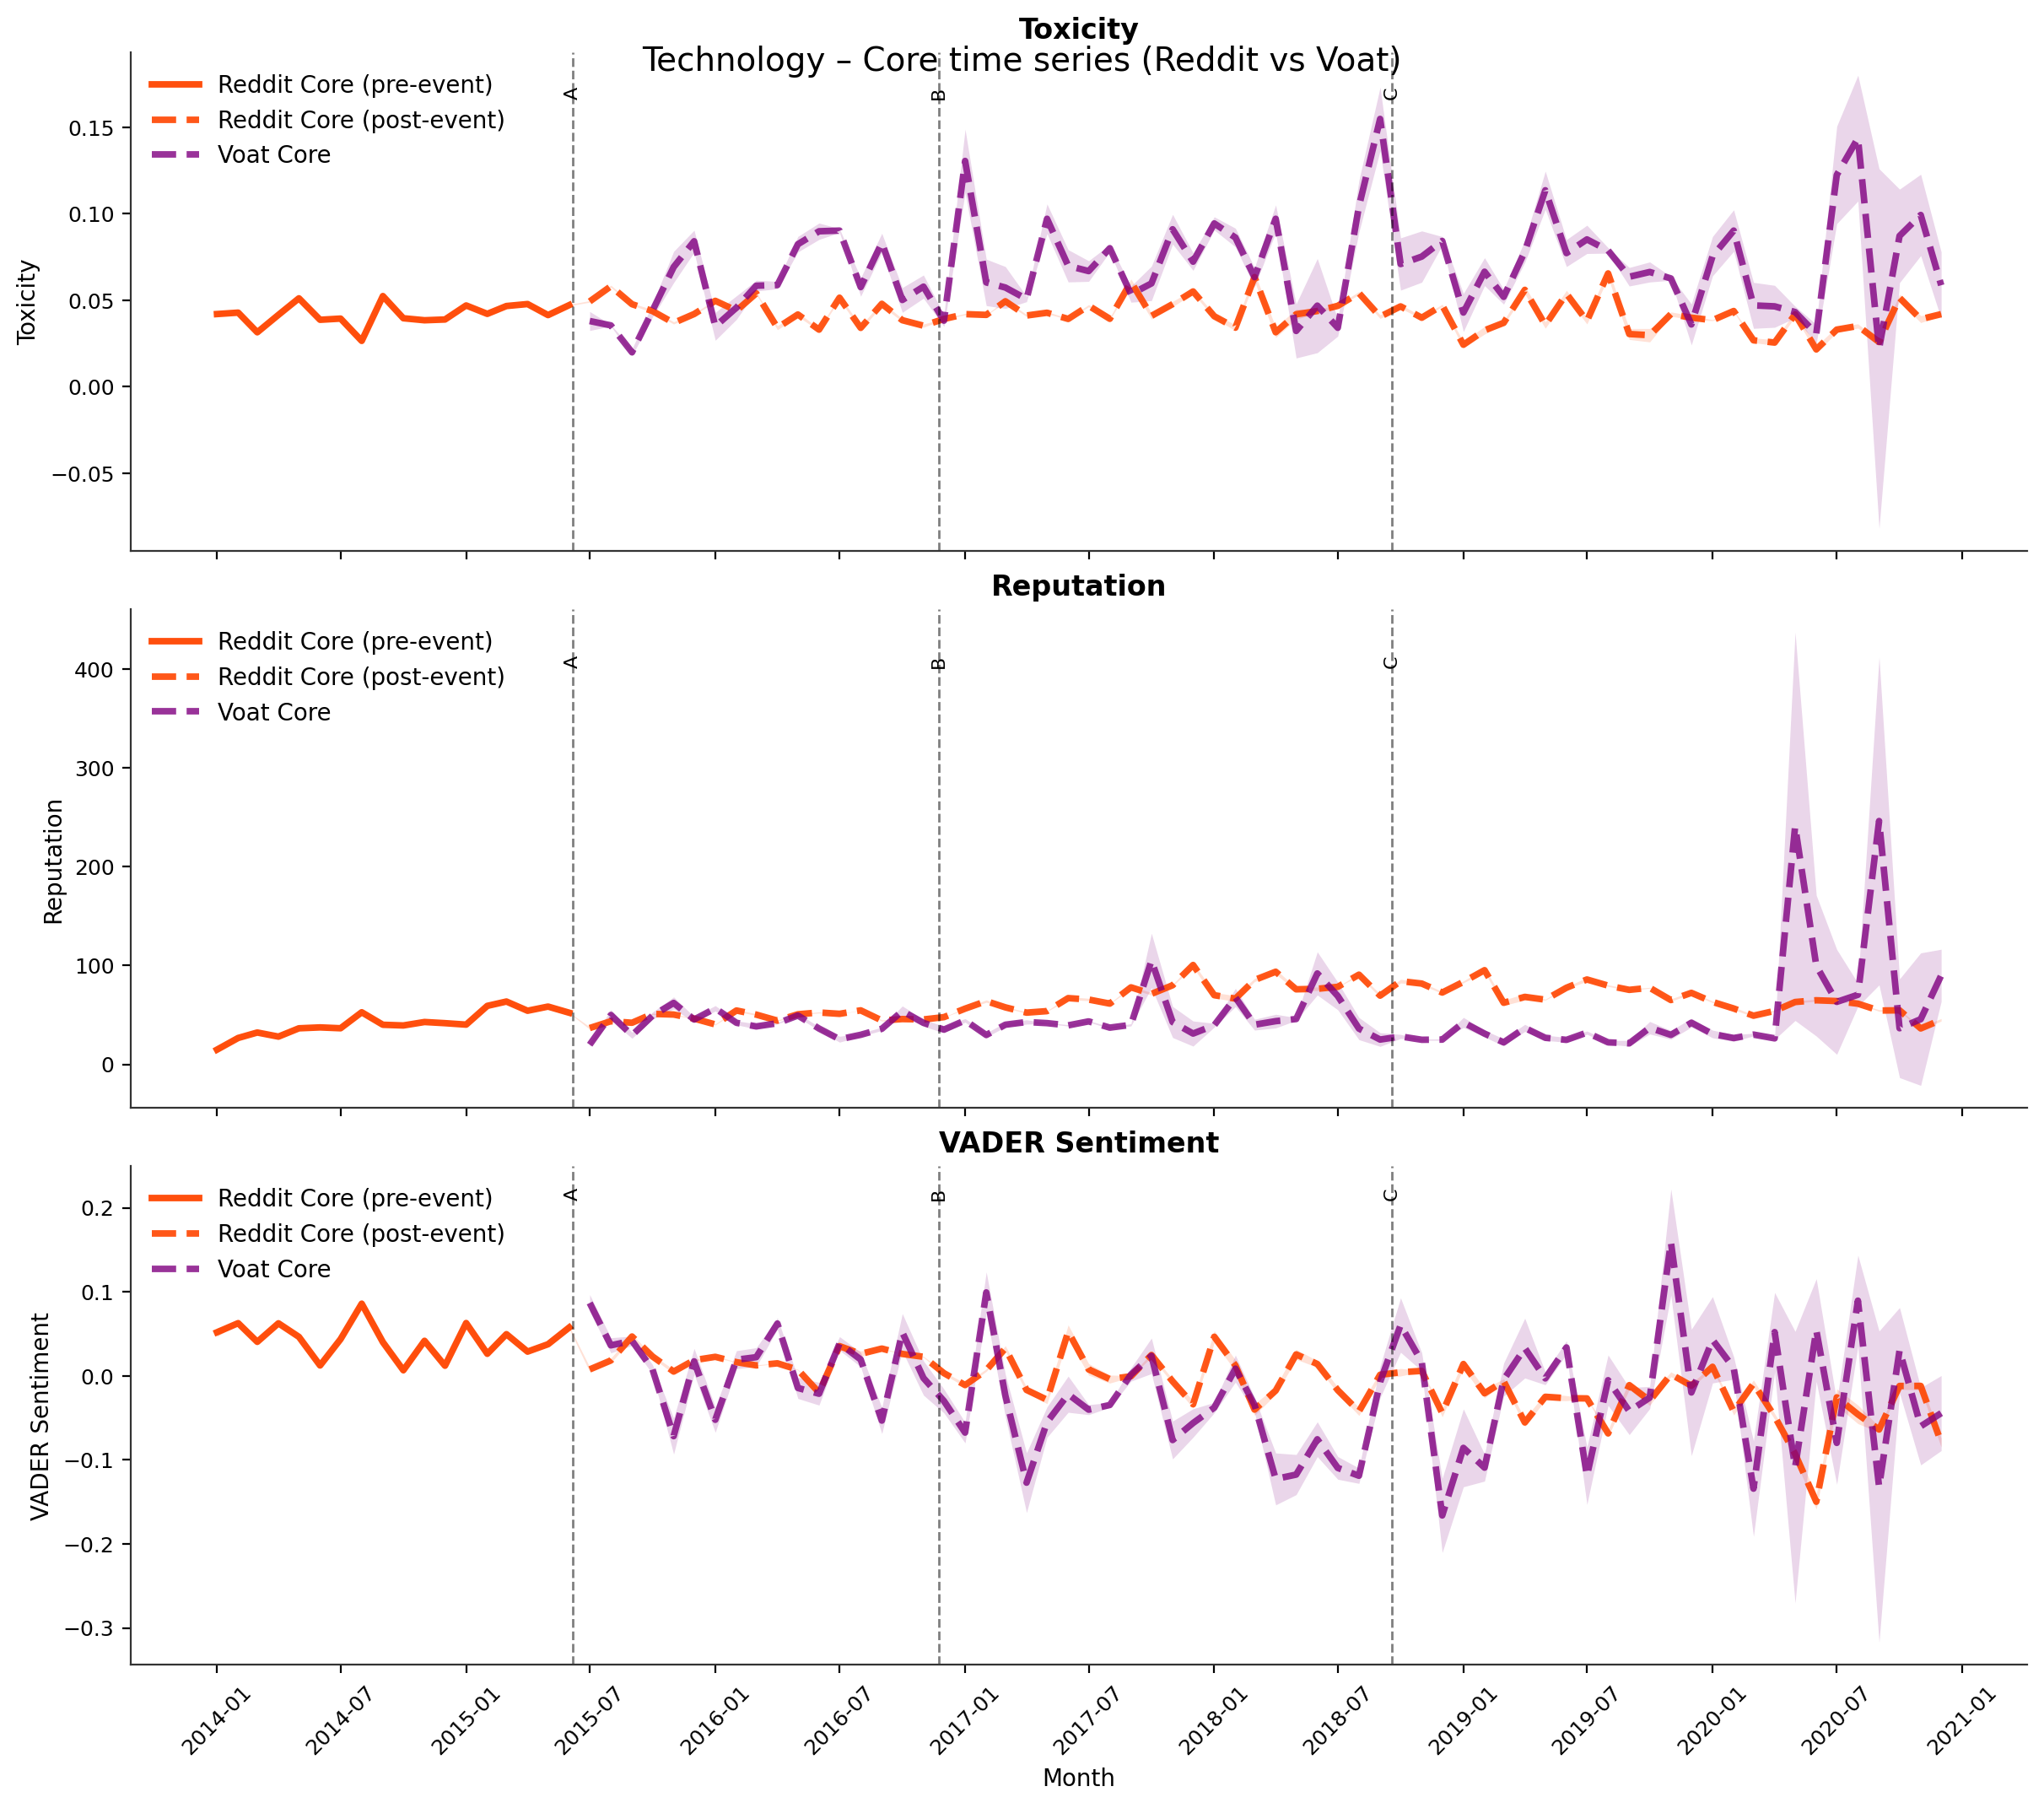
\includegraphics[width=\textwidth]{results/basic/technology/compare/figures/technology_timeseries_panels.png}
\end{frame}

\begin{frame}{Key Insights: Technology Community}
\begin{itemize}
    \item \textbf{Toxicity convergence}: Both platforms show similar modest toxicity ($\sim$0.04-0.05), with Voat only slightly elevated (0.05-0.10)—technology discussions appear more resistant to radicalization than entertainment communities
    \item \textbf{Late reputation anomaly}: Voat Core reputation remains flat (20-40) until a dramatic 250+ spike in late 2020, suggesting either measurement artifact or brief influx of high-status users near platform shutdown
    \item \textbf{Parallel sentiment decline}: Both Reddit and Voat cores trend increasingly negative after 2018, converging around -0.10 by 2020—possibly reflecting broader tech discourse polarization independent of platform
\end{itemize}
\end{frame}

% -------------------------------------------------------------------
% Videos Community
% -------------------------------------------------------------------
\begin{frame}{Videos Community}
\centering
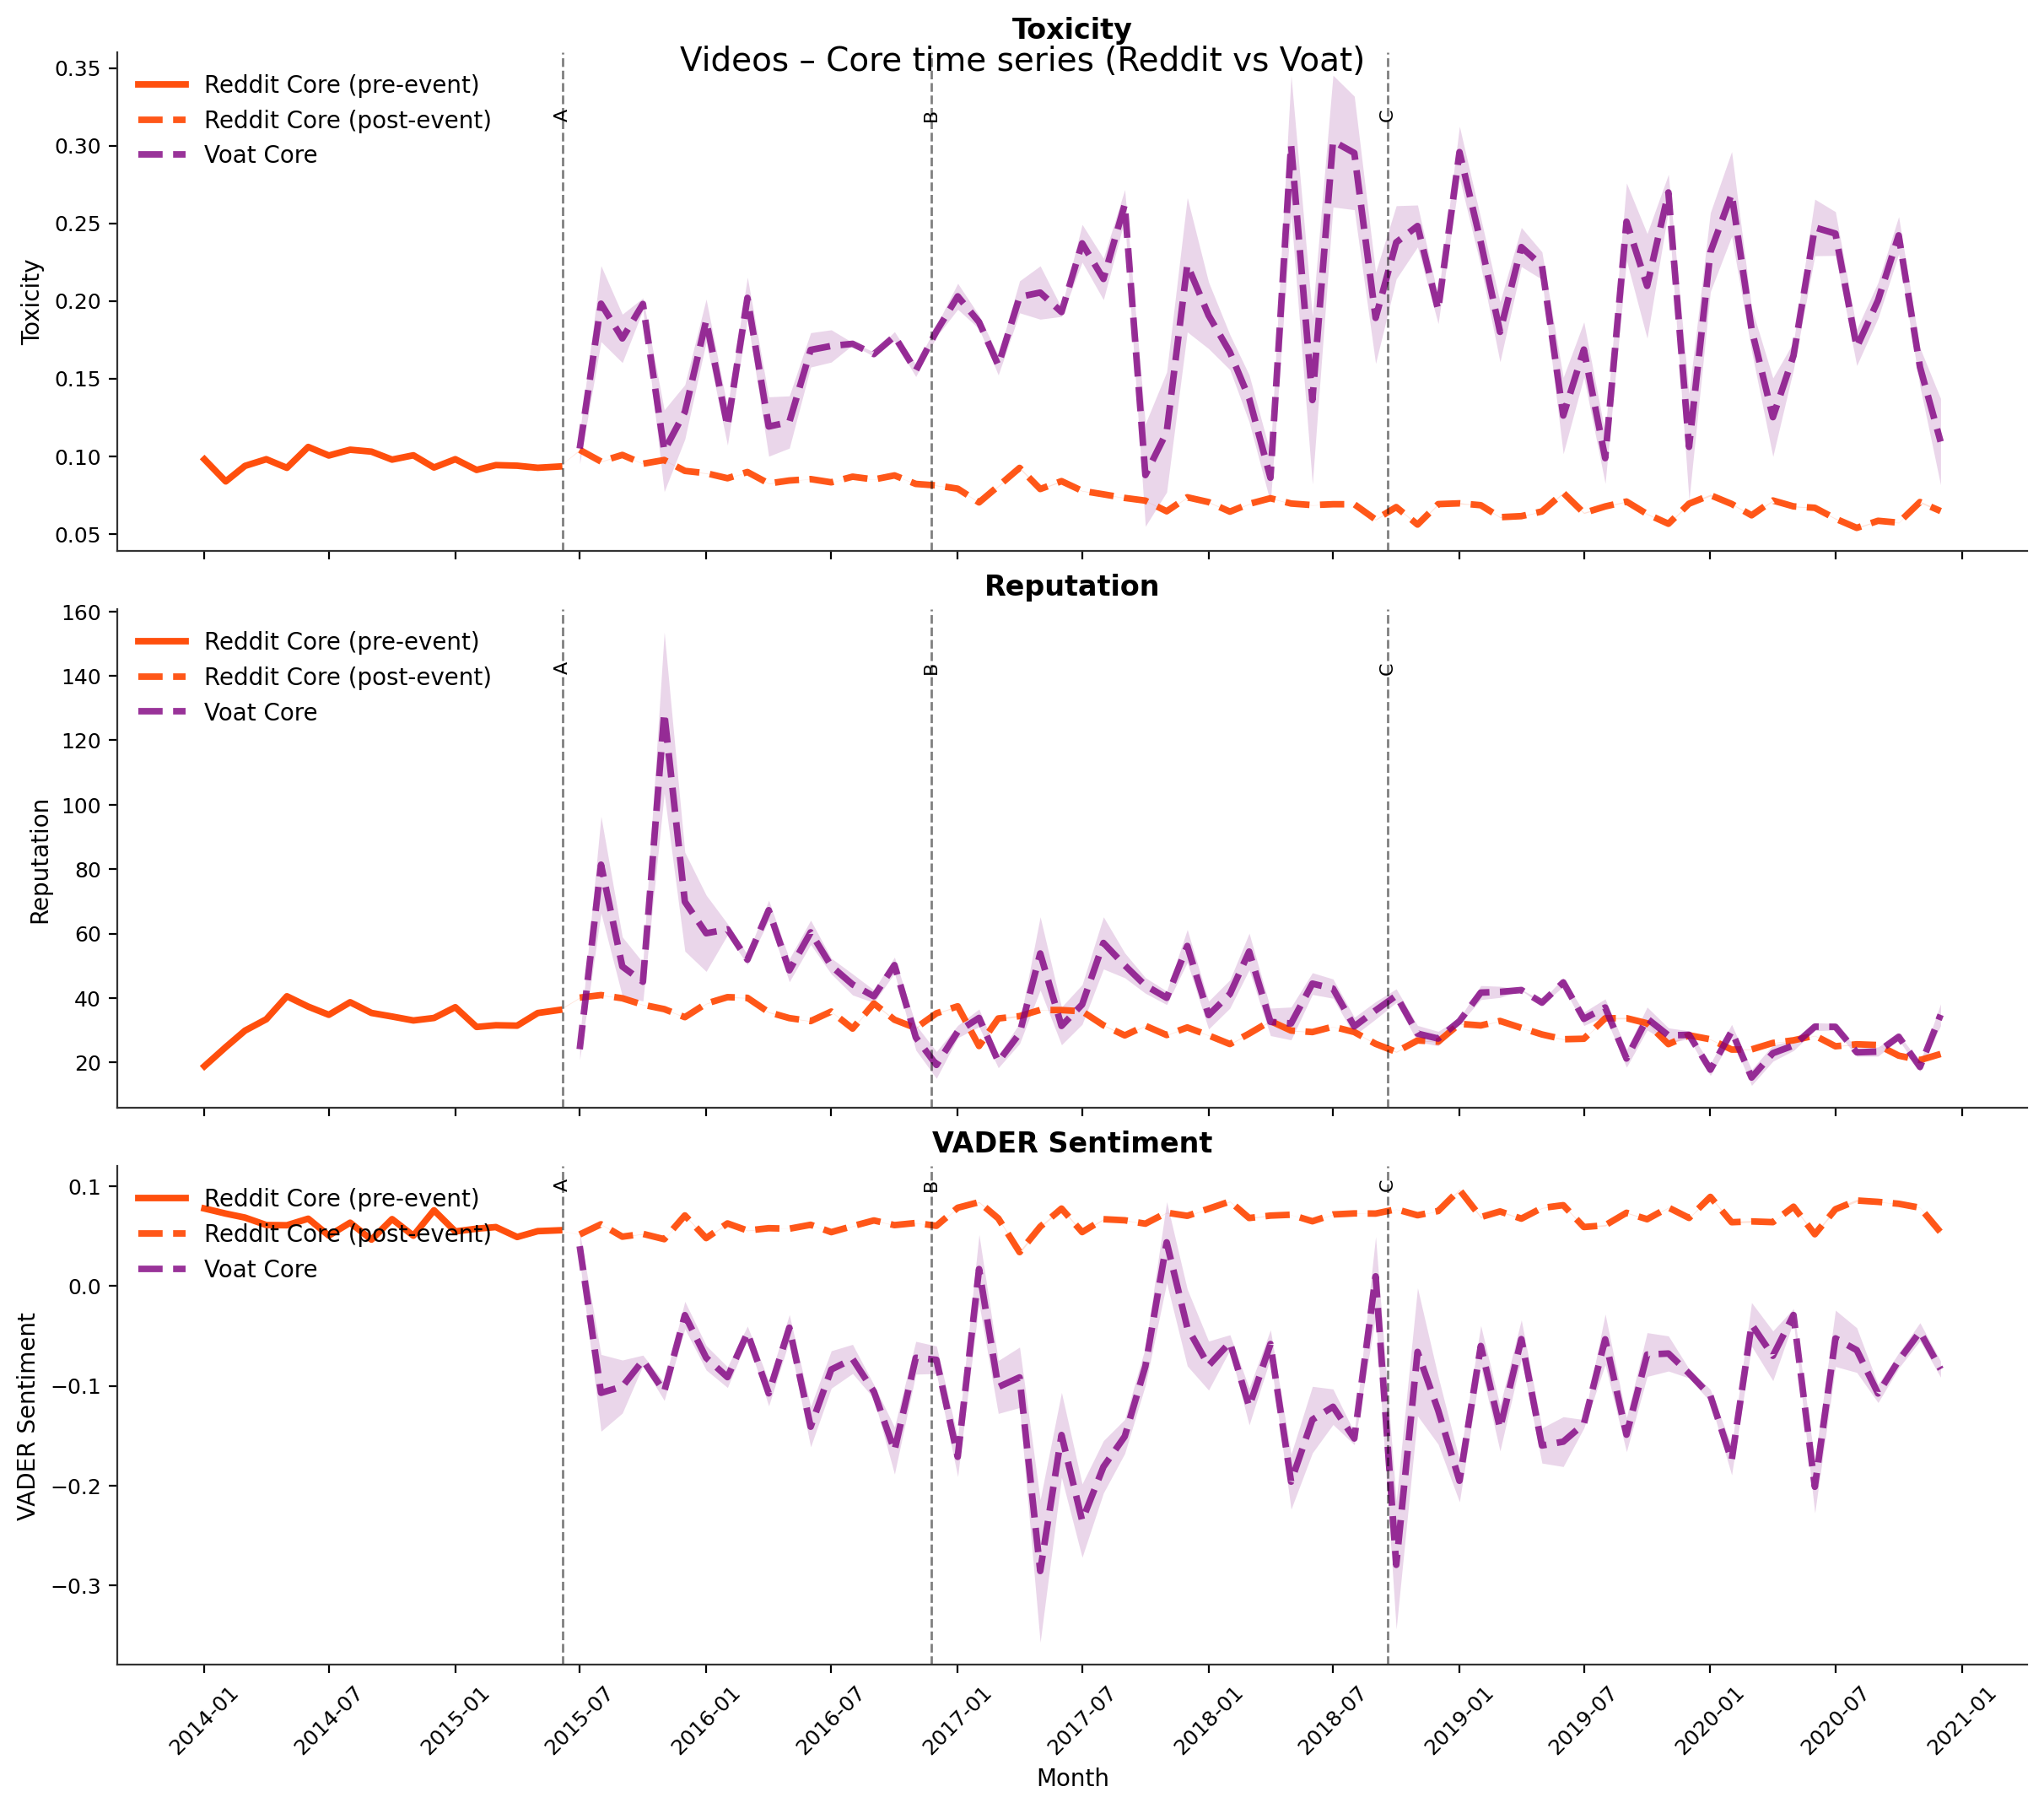
\includegraphics[width=\textwidth]{results/basic/videos/compare/figures/videos_timeseries_panels.png}
\end{frame}

\begin{frame}{Key Insights: Videos Community}
\begin{itemize}
    \item \textbf{Immediate and sustained toxicity gap}: Voat Core toxicity jumps to 0.15-0.20 at Event A and escalates to 0.20-0.30 range, 3-4x Reddit's stable $\sim$0.07—videos became a toxic content haven from the start
    \item \textbf{Early reputation peak then steady decline}: Voat Core reputation spikes to 125+ at Event A, then gradually decays to converge with Reddit ($\sim$20-30) by 2020, suggesting initial high-reputation migrants left or disengaged
    \item \textbf{Deep negative sentiment}: Voat Core maintains consistently negative affect (-0.10 to -0.25) across entire timeline, while Reddit Core sustains positive sentiment (0.05-0.10)—starkest affective divide among generalist communities
\end{itemize}
\end{frame}


\end{document}
